% PAKETE UND DOKUMENTKONFIGURATION
\documentclass[11pt, a4paper]{article}

% Encoding für Umlaute
\usepackage[utf8]{inputenc}
\usepackage[T1]{fontenc}

% Silbentrennung
\usepackage[ngerman]{babel}

% erweiterte Matheumgebungen und Formelnummer mit Sectionnummer
\usepackage{amsmath}
\numberwithin{equation}{section}

% Braket Notation
\usepackage{braket}

% zusätzliche mathematische Schriftarten
\usepackage{amsfonts}

% verschiedene mathematische Symbole
\usepackage{amssymb}

% Einheiten setzen z.B. \SI{10}{\kilo\gram\meter\per\second\squared}
% Fehler: \SI{10 +- 0,2e-4}{\metre}
\usepackage{siunitx}
\sisetup{
  output-decimal-marker={,},
  separate-uncertainty
}

% Randbreiten
\usepackage[left=3.5cm,right=3.5cm,top=3cm,bottom=3cm,twoside]{geometry}

% Bilder einfügen
\usepackage{graphicx}

% Verweise innerhalb des Dokuments
\usepackage{hyperref}
\hypersetup{
	colorlinks = true,
	allcolors = {black}
}

% bessere Tabellenlayouts
\usepackage{booktabs}
\usepackage{multirow}

% Seitenlayout (Kopfzeile)
\usepackage{fancyhdr}

% Float Barriers
\usepackage{placeins}

% Pakete für gedrehte Subfigures
\usepackage{caption}
\usepackage{subcaption}
\usepackage{rotating}

% Caption-Setup
\captionsetup{font={small}}
\renewcommand{\thefigure}{\thesection.\arabic{figure}}
\renewcommand{\thesubfigure}{\alph{subfigure}}
\renewcommand{\thetable}{\thesection.\arabic{table}}
\renewcommand{\thesubtable}{\alph{subtable}}

% Manuelle Silbentrennung
\hyphenation{Halb-werts-brei-te Fa-bry-Pé-rot-E-ta-lon Zee-man-E-ffekt Cad-mi-um-Lam-pe Kon-den-sor-lin-se}

% Tiefe des Inhaltsverzeichnisses (Level: 1 sections, 2 subsections,
% 3 subsubsections)
\setcounter{tocdepth}{3}

% FANCYHDR SETUP
\pagestyle{fancy}
\fancyhead[EL,OR]{\thepage}
\fancyhead[ER]{\leftmark}
\fancyhead[OL]{\rightmark}

\renewcommand{\sectionmark}[1]{
\markboth{Abschnitt \thesection{}: #1}{\thesection{} #1}
}
\renewcommand{\subsectionmark}[1]{
\markright{\thesubsection{} #1}
}

% DOKUMENTINFORMATIONEN
\title{P402 \\ Quantelung von Energie}

\author{Christopher Deutsch\footnote{christopher.deutsch@uni-bonn.de} \and Christian Bespin\footnote{christian.bespin@uni-bonn.de}}

\date{\today}

\begin{document}

\begin{titlepage}

\maketitle

% DURCHFÜHRUNGSDATUM UND ASSISTENT
\begin{center}
\begin{tabular}{l r}
Durchführung: & 1./2. Dezember 2014 \\
Gruppe: & $\alpha$ 2 \\
Assistent: & Dennis Sauerland
\end{tabular}
\end{center}

% ZUSAMMENFASSUNG
\begin{abstract}
\noindent

\end{abstract}

\end{titlepage}

% INHALTSVERZEICHNIS
\tableofcontents
% Neue Seite nach TOC
\newpage

% INHALT VERSUCHSPROTOKOLL

\section{Grundlagen / Theorie}

\subsection{Photoelektrischer Effekt}
\label{ssec:photoeffekt}
Der Begriff \emph{Photoeffekt} umfasst drei verschiedene Arten der Wechselwirkung von Licht mit Materie.
Betrachtet wird der äußere photoelektrische Effekt, das heißt das Herauslösen von Elektronen aus Metalloberflächen (oder Halbleiter) durch Photonen.
Um ein Elektron aus dem Material zu lösen, muss die Austrittsarbeit überwunden werden.
Man stellt fest, dass die auf das Elektron übertragene Energie unabhängig von der Intensität des Lichts ist, was ein Widerspruch der klassischen Theorie der elektromagnetischen Strahlung ist.
Darüber hinaus stellt man fest, dass diese nur von der Frequenz $\nu$ der Strahlung abhängt.
Erstmalig wurde dies durch Einstein (1905 Nobelpreis) als Quantisierung der Energie des Lichts in sogenannte Photonen mit einer Energie:
\begin{align}
	E_\gamma = h \cdot \nu
\end{align}
gedeutet.

\subsection{Photozelle}

\subsubsection{Aufbau und Wirkung}
Die Photozelle ist eine Form der Elektronenröhre, bei der zwei Elektroden in einem evakuierten Glaskolben (um große mittlere freie Weglänge $\Lambda$ zu erreichen) befestigt sind.
Eine der Elektroden bildet die Photokathode, aus der die Elektronen durch Lichteinfall (siehe \ref{ssec:photoeffekt}) ausgelöst werden.
\begin{figure}[h]
\centering
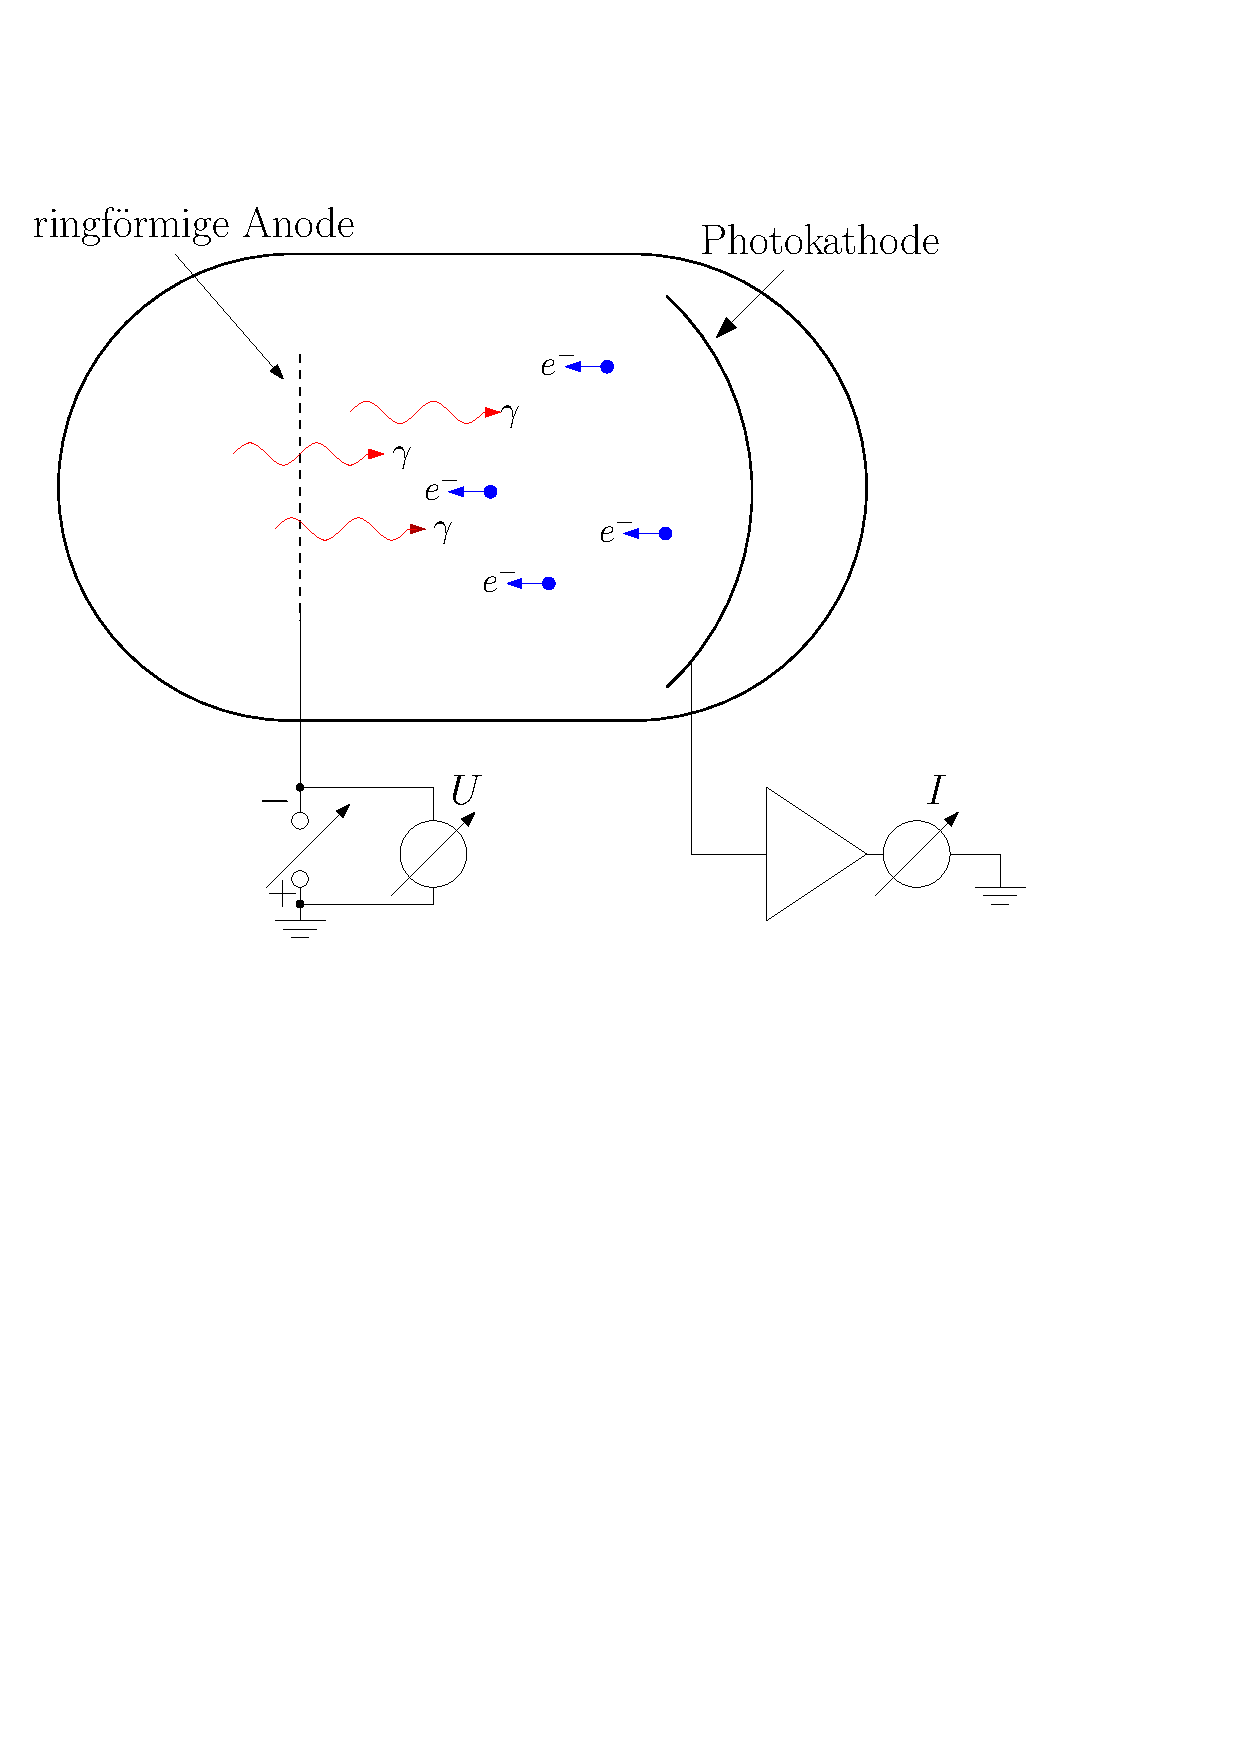
\includegraphics[width=0.65\textwidth]{./figures/aufbau_photozelle.pdf}
\caption{Aufbau einer Photozelle mit Beschaltung der Gegenfeldmethode}
\label{fig:aufbau_photozelle}
\end{figure}
Die Anode ist dabei aus einem dünnen Metallring gefertigt, damit die Photonen sie passieren können, ohne auf sie aufzutreffen und dort gegebenenfalls Elektronen auszulösen, was die Messung stark verfälscht.
Um diesem Effekt zusätzlich entgegenzuwirken wird das Material der Anode (in dem Versuch Platin-Rhodium) so gewählt, dass es eine möglichst hohe Austrittsarbeit hat, damit für den Fall von Photoneneinfall keine Elektronen ausgelöst werden können.
Umgekehrt soll die Austrittsarbeit der Kathode gering sein, damit dort viele Elektronen ausgelöst werden können, hierfür wird in dem Versuch Kalium auf einer oxidierten Silberschicht verwendet.
Die Elektronen fliegen zur Anode und erzeugen so einen \textbf{Photostrom}.
Für den Betrieb einer Photozelle sind grundsätzlich zwei Beschaltungen möglich:
\begin{itemize}
\item Bei dem Betrieb mit \textbf{Saugspannung} wird die Anode mit dem positiven Pol der regelbaren Spannungsquelle verbunden, die Kathode mit dem negativen.
So werden die Elektronen zur Anode hin beschleunigt und dort als Strom registriert.
Das Verfahren eignet sich, wenn man einen besonders hohen Photostrom messen will, allerdings lassen sich dabei keine Rückschlüsse auf die Energie der Elektronen/Photonen ziehen.
\item Bei der \textbf{Gegenfeldmethode}, wie wir sie verwenden werden, wird die Kathode positiv geladen und die Anode negativ, so dass die Elektronen in Richtung der Kathode beschleunigt werden.
Es erreichen demzufolge nur noch Elektronen mit Energien größer $e\,U$ die Anode und bei Verschwinden des Photostroms entspricht die kinetische Energie der Elektronen nach dem Auslösen gerade der Energie $e\,U$, da keine Elektronen mehr die Anode erreichen und als Strom registriert werden.
\end{itemize}
In dem Versuch wird nur die Gegenfeldmethode verwendet, um daraus das Plancksche Wirkungsquantum zu bestimmen und die Austrittsarbeit abzuschätzen.
Dies ist möglich, da die Elektronen in der Photokathode die Energie $E_\gamma$ der Photonen absorbieren und erst aus der Kathode austreten können, wenn diese größer ist als die Austrittsarbeit des Kathodenmaterials.
Die Energiebilanz des Elektrons lautet somit:
\begin{align}
E_e = E_\gamma - W_\mathrm{A} = h \cdot \nu - W_\mathrm{A}
\end{align}

\subsubsection{Photostromverlauf}
\begin{figure}[h]
\centering
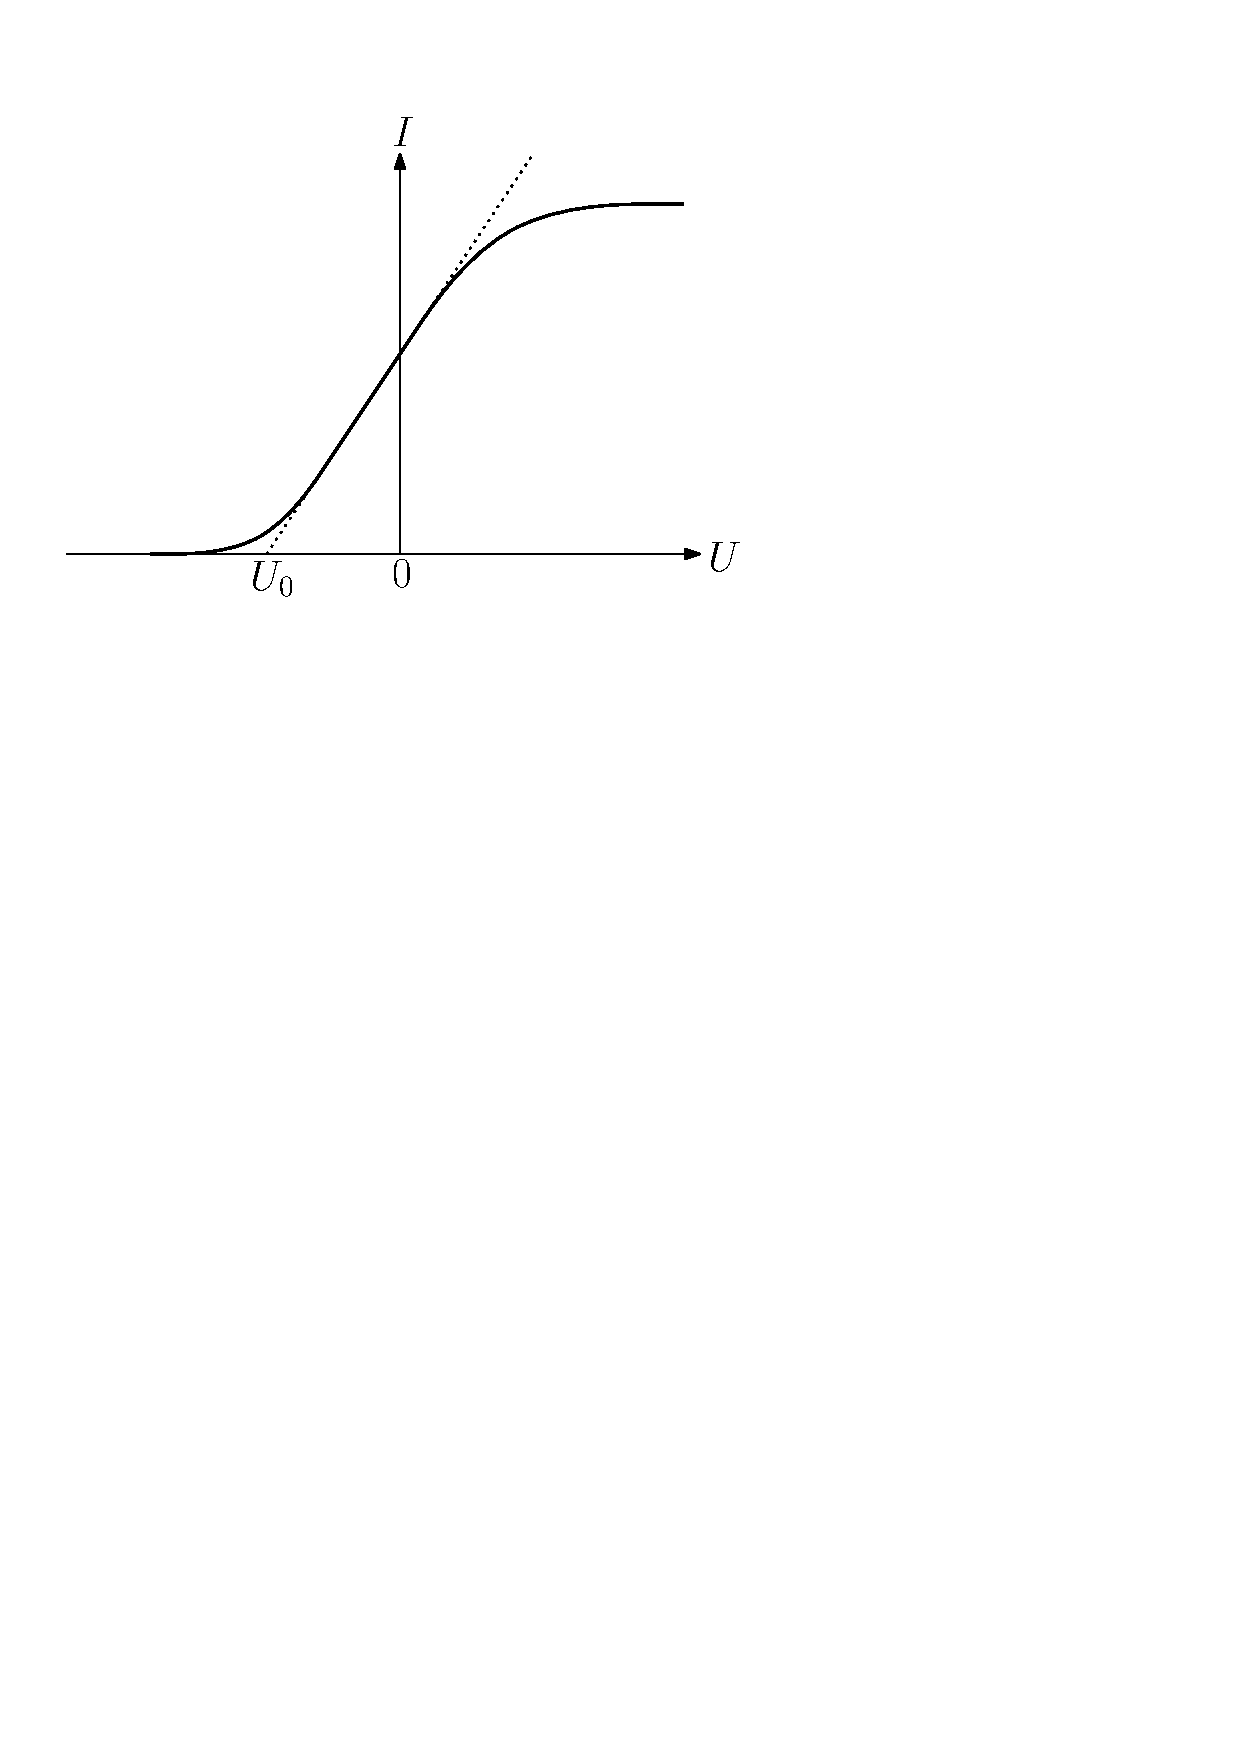
\includegraphics[width=0.5\textwidth]{./figures/kennlinie_photozelle.pdf}
\caption{Qualitative Kennlinie einer Photozelle für Saug- ($U>0$) und Gegenspannungsbetrieb ($U<0$) nach \cite{prak_uheidelberg}}
\label{fig:kennlinie}
\end{figure}
Abbildung \ref{fig:kennlinie} zeigt qualitativ den Verlauf des Anodenstroms in Abhängigkeit der angelegten Spannung. Dabei ist das Vorzeichen so gewählt, dass für $U>0$ der positive Pol der Spannungsquelle an der Anode anliegt (Saugbetrieb).
In dieser Beschaltung erreicht der Strom eine Sättigung bei hohen Spannungen, wenn alle ausgelösten Elektronen die Anode erreichen.
Für Temperaturen über dem absoluten Nullpunkt nähert sich der Photostrom im negativen Spannungsbereich asymptotisch an $0$, wobei für eine ideale Photozelle ein Schnittpunkt mit der $U$-Achse existiert (vgl. \cite{prak_uheidelberg}).
Dort ist auch erwähnt, dass für eine Geometrie wie sie hier vorliegt, der Photostrom im Bereich von $U_0$ folgender Abhängigkeit genügt:
\begin{align}
	I_\mathrm{Photo} \propto (h \nu - e \cdot U_0)^2
\end{align}
Wegen der asymptotischen Annäherung wird darum die Wurzel des Photostroms aufgetragen, um aus der entstehenden linearen Abhängigkeit die Nullstelle $U_0$ extrapolieren zu können, bei der der Photostrom im idealen Fall verschwinden sollte.

\subsubsection{Austrittsarbeit und Kontaktpotential}
\begin{figure}
	\centering
	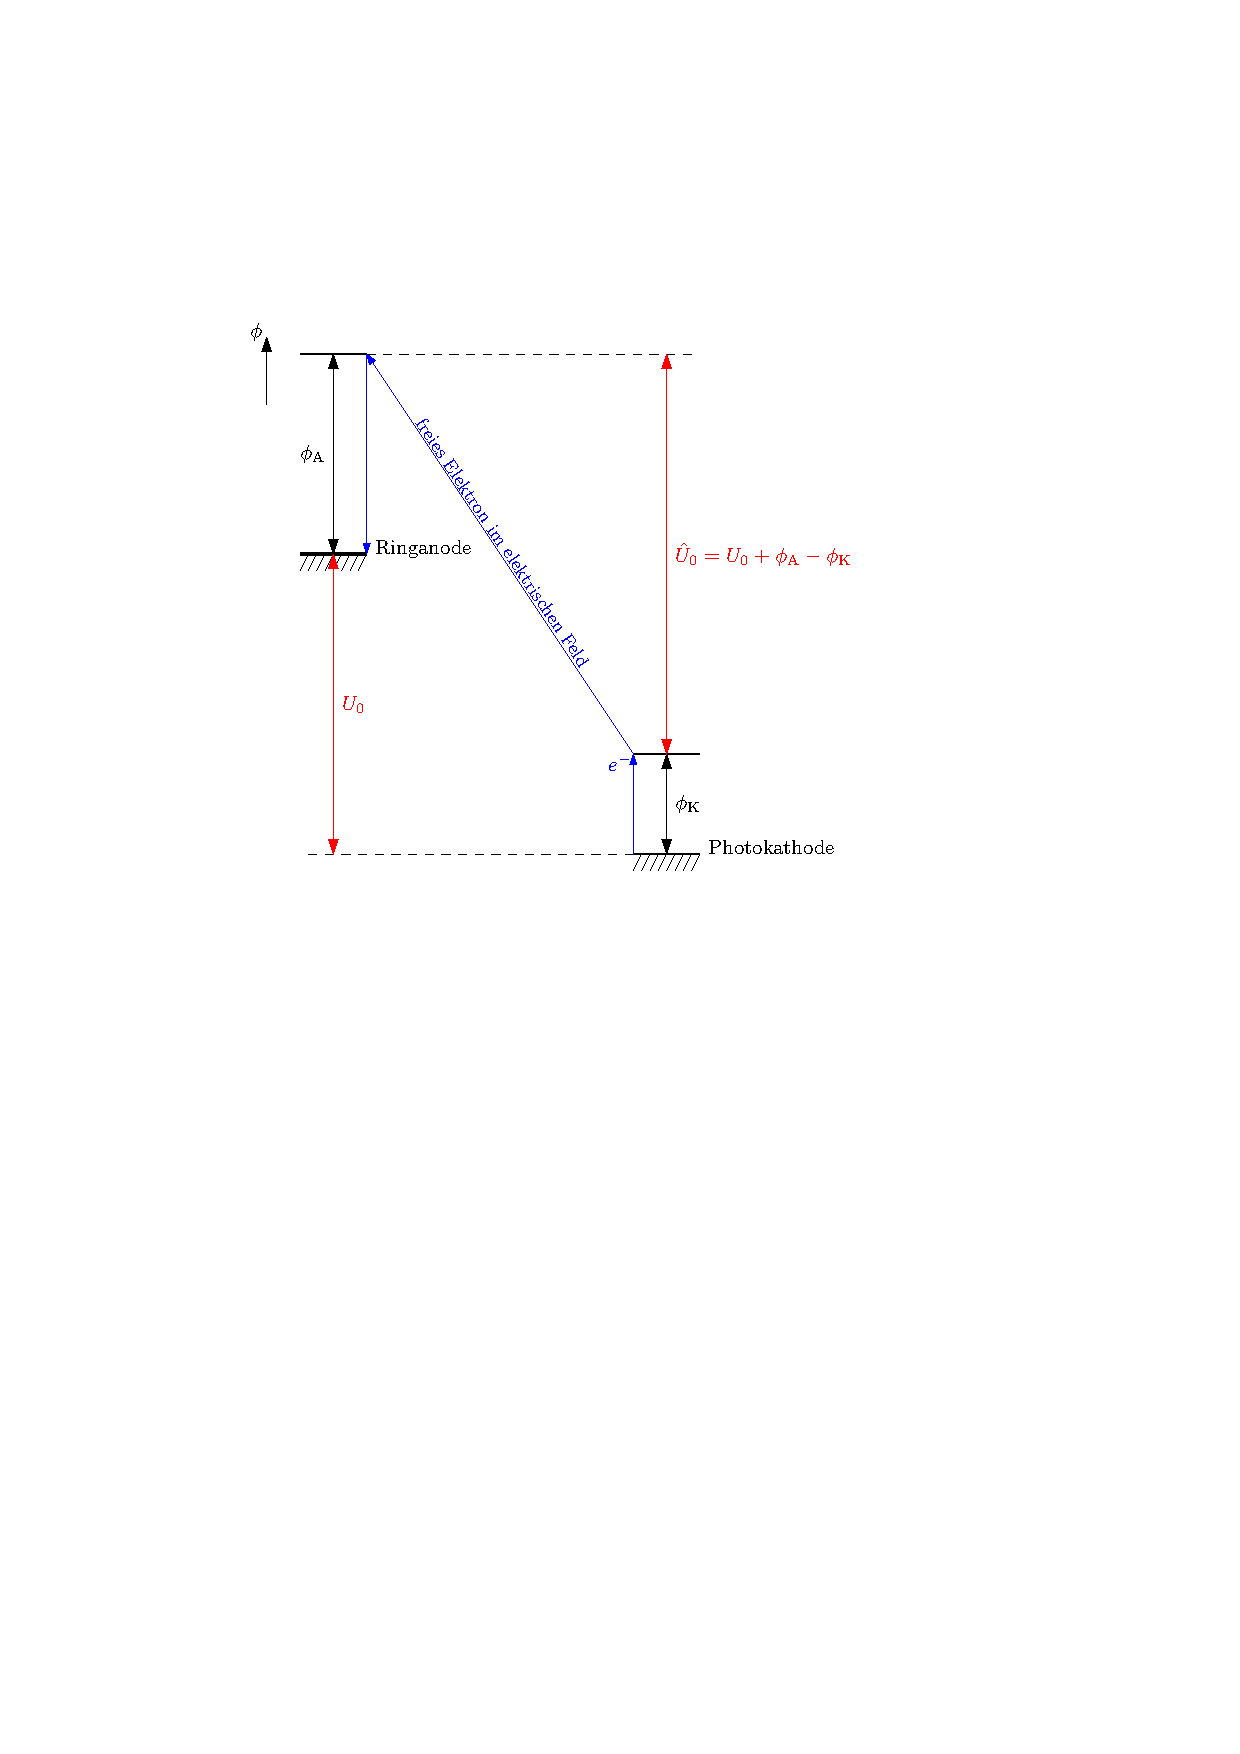
\includegraphics[width=0.8\textwidth]{./figures/kontaktspannung.pdf}
	\caption{schematische Erklärung des Kontaktpotentials}
	\label{fig:kontaktpotential}
\end{figure}
Um ein Elektron aus einem Metall zu lösen, ist eine Mindestenergie erforderlich, die man Austrittsarbeit $W_\mathrm{A}$ nennt.
Drücken wir diese durch ein Austrittspotential $\phi$ aus, so ergibt sich für ein Elektron, welches durch ein Photon der Frequenz $\nu$ aus dem Kathodenmaterial gelöst wurde:
\begin{align}
	E_\mathrm{kin} = h \nu - e \, \phi_\mathrm{K}
\end{align}
Legt man nun zwischen der Ringanode und der Kathode eine Gegenspannung an, so ist die Grenzspannung $U_0$, bei der keine Elektronen mehr bei der Anode ankommen, gegeben durch:
\begin{align}
	E_\mathrm{kin} \stackrel{!}{=} e \, \hat{U}_0 = e \cdot \left( U_0 + \phi_\mathrm{A} - \phi_\mathrm{K}\right)
\end{align}
Insbesondere ist die Potentialdifferenz $\hat{U}_0$, die das Elektron durchlaufen muss, aufgrund der unterschiedlichen Austrittspotentiale von Kathode $\phi_\mathrm{K}$ und Anode $\phi_\mathrm{A}$, nicht gleich der gemessenen Spannung $U_0$.
Dieser Sachverhalt ist in Abbildung \ref{fig:kontaktpotential} schematisch dargestellt.
Die Kontaktspannung $U_\mathrm{Kontakt}$ zwischen zwei Metallen ist gleich der Differenz ihrer Austrittpotentiale, so dass diese im Fall der Photozelle gegeben ist durch:
\begin{align}
	U_\mathrm{Kontakt} = \phi_\mathrm{A} - \phi_\mathrm{K}\text{.}
\end{align}
Mit der Austrittsarbeit der Kathode $W_\mathrm{K} = e \, \phi_\mathrm{K}$ erhält man daraus als Energiebilanz des Elektrons:
\begin{align}
\label{eq:energiebilanz}
	h \nu = e \, U_0 + W_\mathrm{K} + e \, U_\mathrm{Kontakt} \text{,}
\end{align}
und diese ist somit abhängig von der Kontaktspannung zwischen Anode und Kathode.

\subsection{Aufbau der Atomhülle}

\subsubsection{Bohrsches Atommodell}
Das Bohrsche Atommodell ist ein halbklassisches Modell zur Erklärung der diskreten Energieniveaus in Atomen mit einem Elektron.
In diesem wird die Energie durch die Bewegung von Elektron und Kern um den gemeinsamen Schwerpunkt aufgrund des Coulomb-Potentials beschrieben, dabei wird oftmals in guter Näherung der Kern als stationär angenommen.
In diesem klassischen Bild tritt das Problem auf, dass das Elektron schon nach kurzer Zeit in den Kern stürzen sollte, da die Bahn um den gemeinsamen Schwerpunkt eine beschleunigte Bewegung darstellt und dabei Energie in Form von Bremsstrahlung emittiert wird.
Um dieses Problem zu erklären, bediente sich Niels Bohr (1913) der folgenden drei Postulate:
\begin{enumerate}
	\item Es sind nur Bahnen mit Bahndrehimpulsen $L = n \hbar$ erlaubt, wobei $n$ eine natürliche Zahl ist.
	\item Auf diesen Bahnen wird keine Energie abgestrahlt.
	\item Bahnwechsel findet unter Emission beziehungsweise Absorption eines Photons mit der Energie $E_\gamma = E_f - E_i$ statt, wobei $E_f - E_i$ die Energiedifferenz der betrachteten Bahnen ist.
\end{enumerate}
Mithilfe dieser Postulate, ist es möglich die Energie der Bahnen zu bestimmen, wobei sich hier auf einen Kern mit Ladungszahl $Z = \num{1}$ beschränkt werden soll:
\begin{align}
	\label{eq:energieniveaus_bohr}
	E_n = - \frac{1}{2} \, \frac{1}{n^2} \, \alpha^2 \mu c^2 \text{,}
\end{align}
mit der Feinstrukturkonstante $\alpha$:
\begin{align}
	\alpha = \frac{e^2}{4 \pi \epsilon_0 \hbar c}
\end{align}
und der reduzierten Masse $\mu$ des Systems Elektron-Kern:
\begin{align}
	\mu = \frac{m_e \cdot m_\mathrm{K}}{m_e + m_\mathrm{K}}
\end{align}
Die quantenmechanische Behandlung von zwei Punktladungen im gemeinsamen Coulomb-Potential führt im Schwerpunktssystem mit der Relativkoordinate $\vec{r}$ auf den Hamiltonian:
\begin{align}
	\mathcal{H} = - \frac{\hbar}{2 \mu} \nabla^2 - \frac{e^2}{4 \pi \epsilon_0 |\vec{r}|} \text{.}
\end{align}
Die Energieniveaus ergeben sich nun aus der Lösung der stationären Schrödingergleichung:
\begin{align}
	\mathcal{H} \psi = E \psi
\end{align}
und führt auf die Quantenzahlen $n, \ell, m_\ell$ mit Energieeigenwerten wie sie vom Bohr-Modell vorhergesagt wurden (Gleichung \ref{eq:energieniveaus_bohr}).
Bei der quantenmechanischen Lösung beschreibt die Hauptquantenzahl $n$ jedoch nicht den Bahndrehimpuls des Teilchens, sondern die Drehimpulsquantenzahl $\ell$ sowie die magnetische Quantenzahl $m_\ell$, welche die Projektion des Drehimpulses auf eine frei wählbare Quantisierungsachse beschreibt.

\subsubsection{Rydberg-Formel und Balmer-Serie}
\label{sssec:rydberg}
Bereits vor der Beschreibung des Spektrums von Wasserstoff durch Bohr wurden die Übergänge zwischen den Bahnen von Rydberg empirisch durch die sogenannte Rydberg-Formel beschrieben:
\begin{align}
	\label{eq:rydberg_formel}
	\frac{1}{\lambda} = R \cdot \left( \frac{1}{n_f^2} - \frac{1}{n_i^2} \right) \text{,}
\end{align}
wobei $R$ die Rydberg-Konstante in Einheiten einer Wellenzahl bezeichnet.
Nach der theoretischen Beschreibung durch Bohr konnte diese berechnet werden.
Betrachtet man einen Übergang von einem Niveau $E_i$ nach $E_f$, so ist die in Form eines Photons freigewordene Energie:
\begin{align}
	\Delta E = \frac{h c}{\lambda} = E_i - E_f \text{.}
\end{align}
Nutzt man Gleichung \ref{eq:energieniveaus_bohr} und formt nach $\frac{1}{\lambda}$ um, so erhält man:
\begin{align}
	\frac{1}{\lambda} = \frac{1}{2} \, \frac{\alpha^2 \mu c}{h} \left( \frac{1}{n_f^2} - \frac{1}{n_i^2}\right)
\end{align}
und kann die Rydberg-Konstante direkt ablesen:
\begin{align}
\label{eq:rydberg_konstante}
R(\mu) = \frac{1}{2} \, \frac{\alpha^2 \mu c}{h} = \frac{\mu e^4}{8 c \epsilon_0^2 h^3}
\end{align}
Sie hängt insbesondere von der reduzierten Masse des Elektron-Kern-Systems ab.
Vernachlässigt man die Schwerpunktsbewegung so erhält man mit $\mu \approx m_e$ die Rydberg-Konstante bei unendlicher Kernmasse \cite{CODATA}:
\begin{align}
	R_\infty = \SI{10973731.568539 +- 0.000055}{\per\metre}
\end{align}
Offensichtlich hängt die Rydberg-Konstante und damit auch das Emissionsspektrum von der reduzierten Masse $\mu$ ab (Gleichung \ref{eq:rydberg_formel}), wobei die Abhängigkeit durch:
\begin{align}
	R = \frac{\mu}{m_e} \cdot R_\infty = \frac{R_\infty}{1 + \frac{m_e}{m_\mathrm{K}}}
\end{align}
ausgedrückt werden kann.
Aufgrund dieses Zusammenhangs kommt es bei Beobachtung einer Mischung von Wasserstoff und Deuterium zu einer \textbf{Isotopieaufspaltung} des Wasserstoffspektrums, da die Rydberg-Konstante für Deuterium ($m_\mathrm{K} \approx m_\mathrm{p} + m_\mathrm{n}$) etwas größer ist, als die von einfachem Wasserstoff ($m_\mathrm{K} = m_\mathrm{p}$) und somit die Emission von Deuterium bei etwas höherer Energie stattfindet als die des Wasserstoff.

Man klassifiziert aus historischen Gründen Übergänge oft nach ihrem Endniveau $n_f$, sodass diese für $n_i > n_f$ in sogenannte Serien eingeordnet werden.
Für Wasserstoff sind diese: Lyman ($n_i \rightarrow 1$), Balmer ($n_i \rightarrow 2$), Paschen ($n_i \rightarrow 3$), \dots\\
In diesem Versuch werden einige Linien der Balmer-Serie beobachtet, da nur diese Emissionen im optisch sichtbaren Bereich aufweist.

\subsection{Spektroskopie}
\subsubsection{Spektroskopisches Auflösungsvermögen}
\label{sssec:aufloesungsvermoegen}
Das spektroskopische Auflösungsvermögen $\mathcal{R}$ ist definiert als das Verhältnis der Wellenlänge $\lambda$ zur Wellenlängendifferenz $\Delta \lambda$ von zwei gerade noch auflösbaren Linien.
\begin{align}
\mathcal{R} = \frac{\lambda}{\Delta \lambda}
\label{eq:aufloesung}
\end{align}
Gerade noch auflösbar heißt dabei, dass das Rayleigh-Kriterium erfüllt ist, welches besagt, dass der Abstand zweier Intensitätsmaxima $\Delta \lambda$ genau der Halbwertsbreite des Intensitätsverlaufs entspricht.

\subsubsection{Optisches Gitter}
\begin{figure}
	\centering
	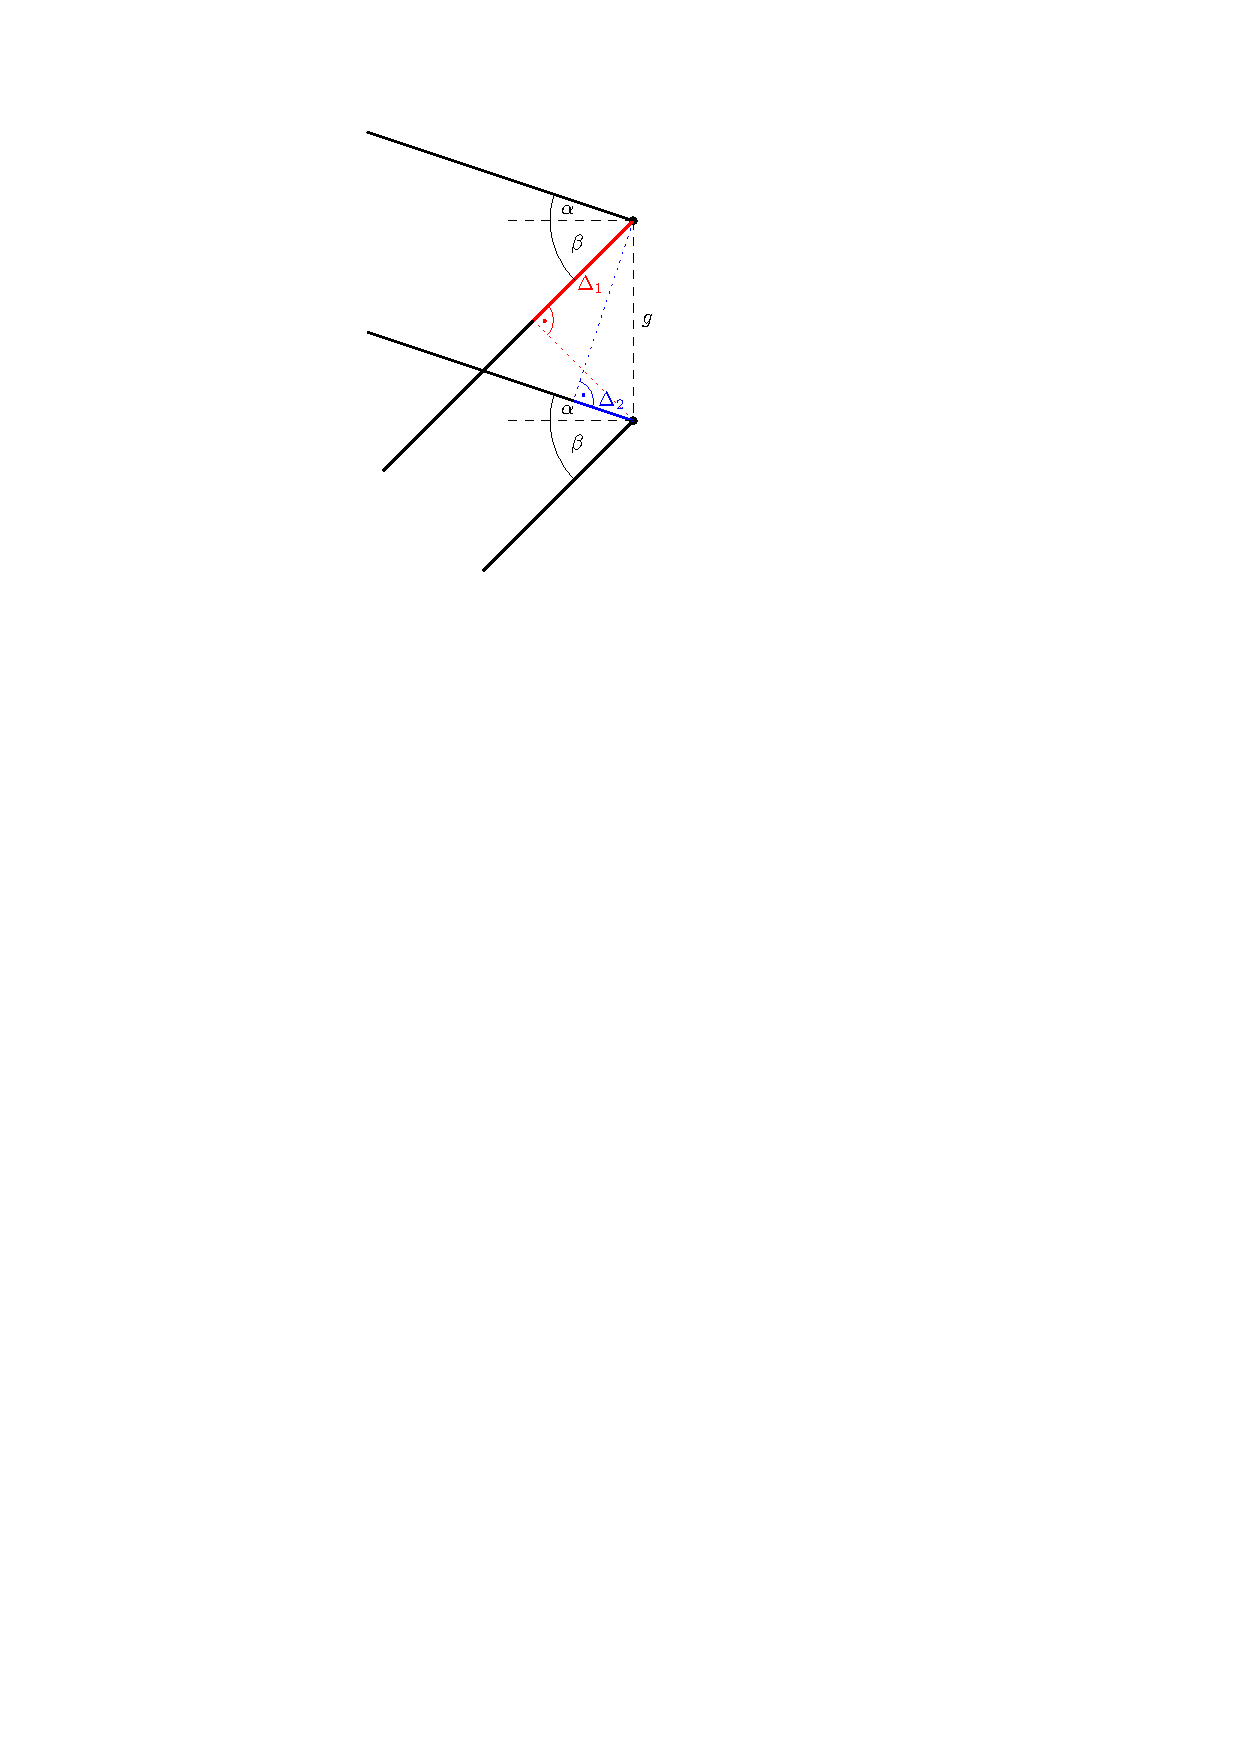
\includegraphics[width=0.4\textwidth]{./figures/herleitung_gitter.pdf}
	\caption{Zur Herleitung der Gittergleichung}
	\label{fig:gitter}
\end{figure}
Ein optisches Gitter besteht aus einer regelmäßigen Anordnung von parallelen Spalten, welche je nach Gittertyp reflektierend oder transmittierend sind.
Das Gitter ist ein wichtiges Instrument zur Spektroskopie, da es aufgrund von Beugung und Interferenz einen von der Wellenlänge abhängigen Transmissions- / Reflexionswinkel aufweist.
Betrachtet man ein Reflexionsgitter mit Spaltabstand $g$ (Gitterkonstante) wie in Abbildung \ref{fig:gitter} so erhält man:
\begin{align}
	\sin(\alpha) = \frac{\Delta_2}{g} \qquad \sin(\beta) = \frac{\Delta_1}{g} \text{,}
\end{align}
sodass der Weglängenunterschied zweier benachbarter Strahlen $\Delta$ gegeben ist durch:
\begin{align}
	\Delta = \Delta_2 - \Delta_1 = g \cdot \left(\sin(\alpha) - \sin(\beta) \right)
\end{align}
Im Gegensatz zu den Verhältnissen in der Zeichnung, wird $\beta$ in gleicher Richtung wie $\alpha$ gemessen, sodass die Substitution $\beta \rightarrow -\beta$ auf den Weglängenunterschied:
\begin{align}
	\Delta = g \cdot \left(\sin(\alpha) + \sin(\beta) \right)
\end{align}
führt.
Um konstruktive Interferenz zu erreichen, muss der Unterschied $\Delta$ der Wegstrecken ein ganzzahliges Vielfaches $m$ der Wellenlänge $\lambda$ sein, so dass die optische Gittergleichung folgt:
\begin{align}
	m \lambda = g \cdot \left( \sin(\alpha) + \sin(\beta) \right) \quad \text{mit} \quad m \in \mathbb{Z}
\end{align}
Man nennt $m$ die Ordnung der Interferenz.
Berechnet man die Intensität des gebeugten Strahls mittels Beugungsformalismus, so bestimmt man nach dem Rayleigh-Kriterium in Abschnitt \ref{sssec:aufloesungsvermoegen} das Auflösungsvermögen durch die Halbwertsbreite $\Delta \lambda$ der Intensitätsmaxima und erhält:
\begin{align}
	\mathcal{R} = \frac{\lambda}{\Delta \lambda} = m \cdot N \text{,}
\end{align}
wobei $N$ die Anzahl der beleuchteten Spalte ist.

\subsubsection{Natürliche Linienbreite und Linienverbreiterung}
Aufgrund der Heisenbergschen Unschärferelation führt die endliche Lebensdauer $\tau$ angeregter Zustände zu einer Energieunschärfe $\Gamma$ bei der Relaxation des Zustandes.
Die Energieunschärfe ist gegeben durch \cite{demtroder}:
\begin{align*}
\Gamma = \frac{\hbar}{\tau}
\end{align*}
und deren Verlauf wird beschrieben durch das Lorentz-Profil.
Darüber hinaus kommt es zur Dopplerverbreiterung aufgrund der thermischen Bewegung der angeregten Atome.
Die Geschwindigkeitsverteilung der Atome in Beobachtungsrichtung ist gaußförmig um Null, sodass auch die Dopplerverbreitung ein gaußförmiges Profil mit der Halbwertsbreite \cite{demtroder}:
\begin{align}
\delta \lambda = \frac{\lambda_0}{c} \sqrt{\frac{8 k_\mathrm{B} T \ln(2)}{m}}
\label{eq:doppler}
\end{align}
hat.
Die Kombination von natürlicher Linienbreite (Lorentz) und Dopplerverbreiterung (Gauß) führt (durch Faltung) zu einem sogenannten Voigt-Profil.
Neben der Dopplerverbreiterung existiert noch die Druckverbreiterung der Linien aufgrund von Stößen mit Nachbarn eines angeregten Atoms.
Diese führen dazu, dass eine Kollision mit einem angeregten Atom zur verfrühten Emissions eines Photons führt.
Daher reduziert sich die typische Zeitskala der Relaxation des Atoms, sodass gemäß der Heisenbergschen Unschärferelation eine größere Energieunschärfe $\Gamma$ resultiert.
Darüberhinaus folgt aus den Stößen eine Störung des Hamiltonians durch Nachbaratome, welche in leicht verschobenen Energieeigenwerten resultiert und somit auch eine Form von Druckverbreiterung darstellt.


\section{Bestimmung des Planckschen Wirkungsquantums}

\subsection{Durchführung}

\subsubsection{Aufbau und Justage}
\begin{figure}[h]
	\centering
	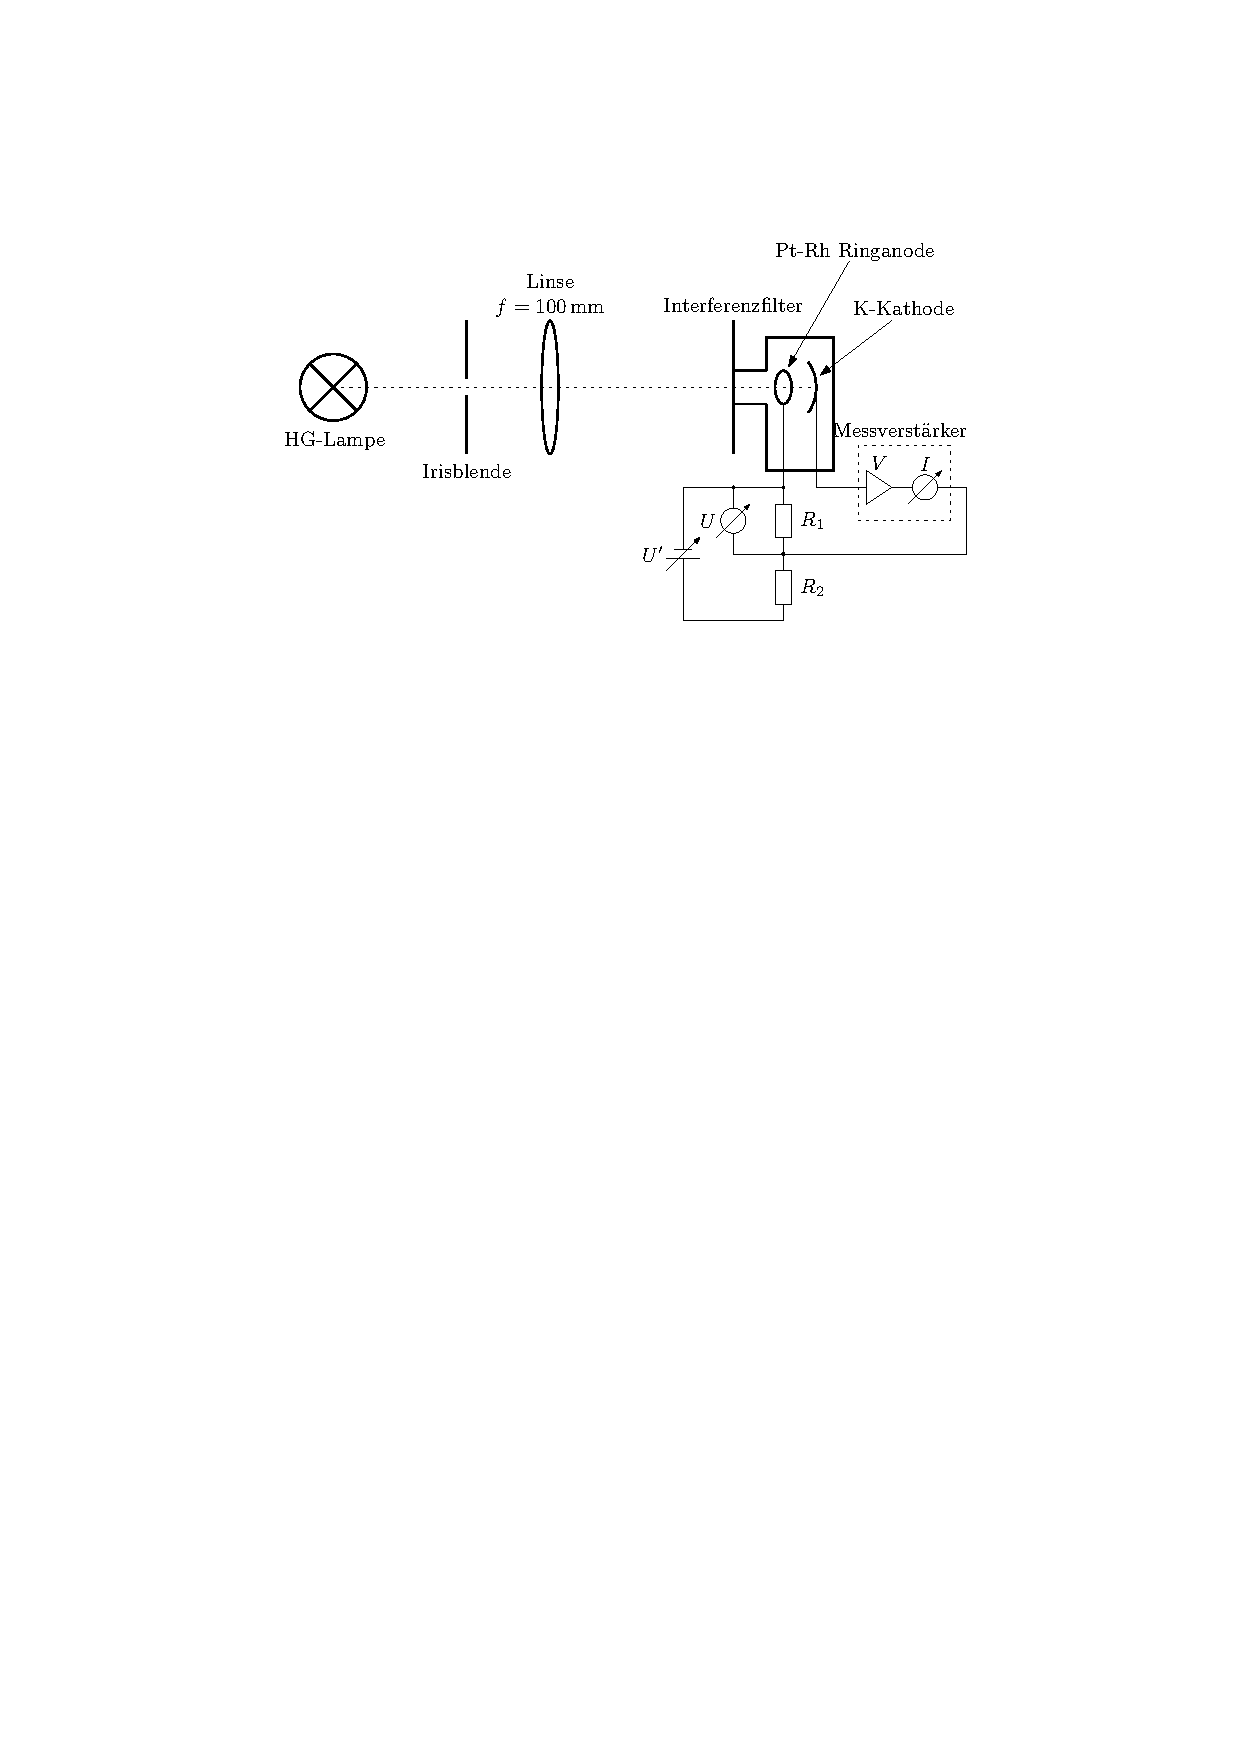
\includegraphics[width=0.9\textwidth]{./figures/versuchsaufbau_photoeffekt.pdf}
	\caption{Versuchsaufbau zur Bestimmung des Planckschen Wirkungsquantums durch den Photoeffekt}
	\label{fig:aufbau_photoeffekt}
\end{figure}
Um das Plancksche Wirkungsquantum zu bestimmen, ist es nötig die Photostrom-Gegenspannungs-Kennlinien ($I$-$U$-Kennlinien) einer Photozelle bei verschiedenen Wellenlängen $\lambda$ zu bestimmen.
Dazu verwenden wir zur Beleuchtung eine Quecksilberdampflampe, welche am Ende der optischen Bank befestigen.
Die vermessene Photozelle stellen wir am anderen Ende der Bank auf.
Um die Intensität des Lichts, welches in die Photozelle fällt regulieren zu können, wird vor die Lampe eine verstellbare Irisblende gestellt.
Zur Fokussierung des Lichts wird die Blende durch eine Linse ($f=\SI{100}{\milli\metre}$) auf die Kathode der Photozelle abgebildet.
Die Wellenlängenselektion erfolgt über ein Interferenzfilterrad, welches direkt vor die Photozelle gestellt wird.

Bei der Justage ist wichtig, dass alle Elemente auf einer optischen Achse liegen.
Dazu schalten wir die Lampe ein und nutzen die Reflexe von Linse und Interferenzfilter um alle Teile auf gleicher Höhe auszurichten.
Wir entfernen außerdem die Schutzkappe von der Photozelle und stellen die Linse so, dass die Blende scharf auf der Kathode abgebildet wird, wobei wir die Irisblende so einstellen, dass der Fleck einen Durchmesser von \num{5} bis \SI{10}{\milli\metre} hat.
Gleichzeitig nutzen wir diese Abbildung um die Höhe der Photozelle einzustellen, wobei wir beachten, dass die Anode nicht beleuchtet wird.
Nach dem Abschluss der Justage wird die Schutzkappe wieder auf die Photozelle gesetzt.

Die Elektronik zur Messung der Kennlinien besteht aus einer regelbaren Spannungsquelle (\num{0}-\SI{12}{\volt}), welche über einem Spannungsteiler die Gegenspannung der Photozelle liefert.
Die Messung des Photostroms erfolgt über einen Messverstärker, welcher eine zum Strom proportionale Spannung ausgibt.
Die im Versuch auftretenden Ströme wurden dabei mit einem Verstärkungsfaktor von $V = \SI{1e-8}{\ampere\per\volt}$ gemessen, wobei der Fehler auf diesen vernachlässigt wird.
Die Messung von Gegenspannung und Photostrom erfolgt dann über zwei Voltmeter, welche die Spannung an Messverstärker beziehungsweise Spannungsteiler messen.

\subsubsection{Messung der Kennlinien}
Zunächst wählen wir den Interferenzfilter mit Mittenwellenlänge $\lambda = \SI{365}{\nano\metre}$ und überprüfen, in welcher Größenordnung sich die Grenzspannung $U_0$, bei der kein Photostrom mehr fließt, befindet.
Diese liegt in der Größenordnung von \SI{2}{\volt}, daher wählen wir einen Spannungsteiler aus \SI{100}{\ohm} und \SI{222}{\ohm}, um die Spannungsquelle feiner zu regeln.

Nun wird mit der Messung der Kennlinien für die Wellenlängen $\lambda = \num{365}$, \num{405}, \num{436}, \num{546} und \SI{578}{\nano\metre} begonnen.
Es wird für jeden Filter wie folgt vorgegangen:
\begin{itemize}
  \item Messung des Anodenphotostroms $I_0$: Es wird der Strom bei maximaler Gegenspannung gemessen, da bei dieser kein Kathodenphotostrom mehr stattfindet.
  Der gemessene Strom entspricht dabei nicht dem Anodenphotostrom, sondern der Summe von Anodenphotostrom und Offset des Verstärkers.
  Der Offset wurde nicht konkret bestimmt, da die gemessenen Kennlinien $I-I_0$ als Differenz zweier offsetbehafteter Größen aufgetragen werden und ein konstanter Versatz somit keinen Einfluss auf die Differenz hat. 
  \item Abschätzung der Grenzspannung $U_0$: Es wird die Gegenspannung langsam verringert bis ein signifikanter Anstieg des Photostroms beobachtet werden kann.
  Die Gegenspannung bei der dies einsetzt, dient als erste Abschätzung der Grenzspannung, so dass der Messbereich entsprechend gewählt werden kann.
  \item Messung der Kennlinie: Es wird bei der Messung bei einer Gegenspannung von $U = \SI{0}{\volt}$ begonnen, welche schrittweise bis zur abgeschätzten Grenzspannung $U_0$ hochgeregelt wird. Dabei wird beachtet, dass ausreichend Messpunkte im quadratischen Bereich der Kennlinie liegen.
\end{itemize}
Nachdem die Kennlinienmessung für jeden Filter einmal durchgeführt wurde, wiederholen wir die Messungen um Intensitätsschwankungen der Quecksilberdampflampe feststellen zu können.

Anschließend wird die Kennlinie der Photozelle bei höherer Intensität vermessen, dabei wird nur der Filter mit Mittelwellenlänge $\lambda = \SI{365}{\nano\metre}$ verwendet.
Dazu wird die Öffnung der Irisblende soweit vergrößert, dass ein signifikanter Anstieg des Photostroms beobachtet werden kann, ohne dabei die Ringanode zu beleuchten.
Analog zum vorigen Teil wird der Anodenphotostrom bei maximaler Gegenspannung gemessen, die Grenzspannung abgeschätzt und gemäß diesem der Messbereich der Kennlinie gewählt.

Es wird der absolute Fehler der Gegenspannungsmessung mit dem Digitalmultimeter konservativ auf $\Delta U = \SI{2}{\milli\ampere}$ abgeschätzt.
Im Gegensatz dazu, konnte eine starke Schwankung der Photostrom-Messung mit dem Messverstärker bei hohen Strömen festgestellt werden.
Daher wird hier ein relativer Fehler von $\frac{\Delta I}{I} = \SI{2}{\percent}$ abgeschätzt

\subsection{Auswertung}
Zunächst wird gemäß des Verstärkerfaktors von $V = \SI{1e-8}{\ampere\per\volt}$ aus der gemessenen Spannung der Photostrom $I$ und der Anodenstroms $I_0$ berechnet.
Es wird auf die Angabe der gemessenen Spannungen verzichtet und stattdessen direkt der Kathodenphotostrom $I-I_0$ angegeben.
Dabei wurde der Fehler $\Delta (I - I_0)$ durch Gaußssche Fehlerfortpflanzung aus den relativen Fehlern $\frac{\Delta I}{I} = \frac{\Delta I_0}{I_0} = \SI{2}{\percent}$ berechnet.
Die Kennlinienmessungen finden sich im Anhang \ref{app:kennlinien}.



\subsubsection{Bestimmung der Grenzspannung $U_0$ für die verschiedenen Wellenlängen}
\label{sssec:photoeffekt_grenzspannung}
Zur Bestimmung der Grenzspannung wird ausgenutzt, dass die Kennlinie im Anlaufgebiet quadratisch mit der Gegenspannung $U$ anwächst.
Daher kann durch Auftragen der Wurzel des Kathodenphotostroms $\sqrt{I-I_0}$ gegen die anliegende Gegenspannung $U$ die Kennlinie linearisiert werden und durch Extrapolation des linearen Teils der Kurve die Grenzspannung $U_0$ als Schnittpunkt mit der $x$-Achse berechnet werden.
Dabei ist zu beachten, dass bei hohen Gegenspannungen eine Abweichung vom quadratischen Zusammenhang zu beobachten ist, welche bei der Extrapolation vernachlässigt wird.
Die Linearisierung wurde in Abbildung \ref{fig:kennlinien_exemp_365nm} exemplarisch aufgetragen, wobei der Fehler gemäß der Gaußsschen Fehlerfortpflanzung bei Bildung der Wurzel berechnet wurde.
\begin{figure}[h]
	\centering
	% GNUPLOT: LaTeX picture with Postscript
\begingroup
  \makeatletter
  \providecommand\color[2][]{%
    \GenericError{(gnuplot) \space\space\space\@spaces}{%
      Package color not loaded in conjunction with
      terminal option `colourtext'%
    }{See the gnuplot documentation for explanation.%
    }{Either use 'blacktext' in gnuplot or load the package
      color.sty in LaTeX.}%
    \renewcommand\color[2][]{}%
  }%
  \providecommand\includegraphics[2][]{%
    \GenericError{(gnuplot) \space\space\space\@spaces}{%
      Package graphicx or graphics not loaded%
    }{See the gnuplot documentation for explanation.%
    }{The gnuplot epslatex terminal needs graphicx.sty or graphics.sty.}%
    \renewcommand\includegraphics[2][]{}%
  }%
  \providecommand\rotatebox[2]{#2}%
  \@ifundefined{ifGPcolor}{%
    \newif\ifGPcolor
    \GPcolortrue
  }{}%
  \@ifundefined{ifGPblacktext}{%
    \newif\ifGPblacktext
    \GPblacktexttrue
  }{}%
  % define a \g@addto@macro without @ in the name:
  \let\gplgaddtomacro\g@addto@macro
  % define empty templates for all commands taking text:
  \gdef\gplbacktext{}%
  \gdef\gplfronttext{}%
  \makeatother
  \ifGPblacktext
    % no textcolor at all
    \def\colorrgb#1{}%
    \def\colorgray#1{}%
  \else
    % gray or color?
    \ifGPcolor
      \def\colorrgb#1{\color[rgb]{#1}}%
      \def\colorgray#1{\color[gray]{#1}}%
      \expandafter\def\csname LTw\endcsname{\color{white}}%
      \expandafter\def\csname LTb\endcsname{\color{black}}%
      \expandafter\def\csname LTa\endcsname{\color{black}}%
      \expandafter\def\csname LT0\endcsname{\color[rgb]{1,0,0}}%
      \expandafter\def\csname LT1\endcsname{\color[rgb]{0,1,0}}%
      \expandafter\def\csname LT2\endcsname{\color[rgb]{0,0,1}}%
      \expandafter\def\csname LT3\endcsname{\color[rgb]{1,0,1}}%
      \expandafter\def\csname LT4\endcsname{\color[rgb]{0,1,1}}%
      \expandafter\def\csname LT5\endcsname{\color[rgb]{1,1,0}}%
      \expandafter\def\csname LT6\endcsname{\color[rgb]{0,0,0}}%
      \expandafter\def\csname LT7\endcsname{\color[rgb]{1,0.3,0}}%
      \expandafter\def\csname LT8\endcsname{\color[rgb]{0.5,0.5,0.5}}%
    \else
      % gray
      \def\colorrgb#1{\color{black}}%
      \def\colorgray#1{\color[gray]{#1}}%
      \expandafter\def\csname LTw\endcsname{\color{white}}%
      \expandafter\def\csname LTb\endcsname{\color{black}}%
      \expandafter\def\csname LTa\endcsname{\color{black}}%
      \expandafter\def\csname LT0\endcsname{\color{black}}%
      \expandafter\def\csname LT1\endcsname{\color{black}}%
      \expandafter\def\csname LT2\endcsname{\color{black}}%
      \expandafter\def\csname LT3\endcsname{\color{black}}%
      \expandafter\def\csname LT4\endcsname{\color{black}}%
      \expandafter\def\csname LT5\endcsname{\color{black}}%
      \expandafter\def\csname LT6\endcsname{\color{black}}%
      \expandafter\def\csname LT7\endcsname{\color{black}}%
      \expandafter\def\csname LT8\endcsname{\color{black}}%
    \fi
  \fi
  \setlength{\unitlength}{0.0500bp}%
  \begin{picture}(6480.00,4320.00)%
    \gplgaddtomacro\gplbacktext{%
      \csname LTb\endcsname%
      \put(946,704){\makebox(0,0)[r]{\strut{} 0}}%
      \csname LTb\endcsname%
      \put(946,1076){\makebox(0,0)[r]{\strut{} 0,5}}%
      \csname LTb\endcsname%
      \put(946,1449){\makebox(0,0)[r]{\strut{} 1}}%
      \csname LTb\endcsname%
      \put(946,1821){\makebox(0,0)[r]{\strut{} 1,5}}%
      \csname LTb\endcsname%
      \put(946,2193){\makebox(0,0)[r]{\strut{} 2}}%
      \csname LTb\endcsname%
      \put(946,2566){\makebox(0,0)[r]{\strut{} 2,5}}%
      \csname LTb\endcsname%
      \put(946,2938){\makebox(0,0)[r]{\strut{} 3}}%
      \csname LTb\endcsname%
      \put(946,3310){\makebox(0,0)[r]{\strut{} 3,5}}%
      \csname LTb\endcsname%
      \put(946,3683){\makebox(0,0)[r]{\strut{} 4}}%
      \csname LTb\endcsname%
      \put(946,4055){\makebox(0,0)[r]{\strut{} 4,5}}%
      \csname LTb\endcsname%
      \put(1078,484){\makebox(0,0){\strut{} 0}}%
      \csname LTb\endcsname%
      \put(2079,484){\makebox(0,0){\strut{} 0,5}}%
      \csname LTb\endcsname%
      \put(3080,484){\makebox(0,0){\strut{} 1}}%
      \csname LTb\endcsname%
      \put(4081,484){\makebox(0,0){\strut{} 1,5}}%
      \csname LTb\endcsname%
      \put(5082,484){\makebox(0,0){\strut{} 2}}%
      \csname LTb\endcsname%
      \put(6083,484){\makebox(0,0){\strut{} 2,5}}%
      \put(176,2379){\rotatebox{-270}{\makebox(0,0){\strut{}$\sqrt{I-I_0} \, / \, \si{\nano\ampere^{1/2}}$}}}%
      \put(3580,154){\makebox(0,0){\strut{}$U \, / \, \si{\volt}$}}%
      \put(3580,3945){\makebox(0,0){\strut{}}}%
    }%
    \gplgaddtomacro\gplfronttext{%
      \csname LTb\endcsname%
      \put(5096,3882){\makebox(0,0)[r]{\strut{}Messung 1}}%
      \csname LTb\endcsname%
      \put(5096,3662){\makebox(0,0)[r]{\strut{}Regressionsgerade 1}}%
      \csname LTb\endcsname%
      \put(5096,3442){\makebox(0,0)[r]{\strut{}Messung 2}}%
      \csname LTb\endcsname%
      \put(5096,3222){\makebox(0,0)[r]{\strut{}Regressionsgerade 2}}%
    }%
    \gplbacktext
    \put(0,0){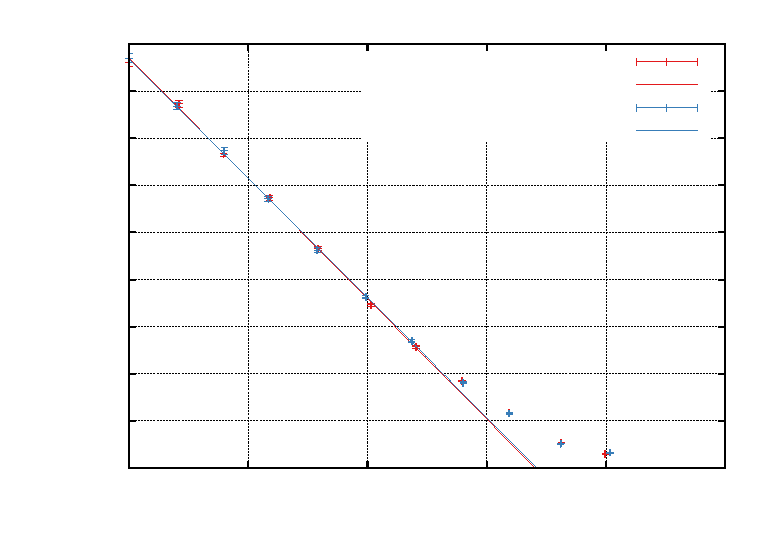
\includegraphics{./plots/photo/kennlinien_365nm}}%
    \gplfronttext
  \end{picture}%
\endgroup

	\caption{Linearisierung der Kennlinie bei einer Wellenlänge von $\lambda = \SI{365}{\nano\metre}$. }
	\label{fig:kennlinien_exemp_365nm}
\end{figure}
Um schließlich die Grenzspannung zu erhalten, wird an den linearen Teil der Kurve eine Gerade mithilfe eines Least-Squares-Verfahrens (\texttt{Gnuplot}) angepasst.
Die restlichen Linearisierungen wurden im Anhang \ref{app:kennlinien} zusammengetragen und die Ergebnisse der Anpassung in Tabelle \ref{tab:photoeffekt_fit_results} zusammengefasst.
\begin{table}[h]
	\centering
	\begin{tabular}{SSSSSSSS}
	\toprule
	{$\frac{\lambda}{\si{\nano\metre}}$} & {$\frac{m}{\si{\nano\ampere\tothe{1/2}\per\volt}}$} & {$\frac{\Delta m}{\si{\nano\ampere\tothe{1/2}\per\volt}}$} & {$\frac{b}{\si{\nano\ampere\tothe{1/2}}}$} & {$\frac{\Delta b}{\si{\nano\ampere\tothe{1/2}}}$} & {$\chi_\mathrm{d.o.f.}^2$} & {$\frac{U_G}{\si{\volt}}$} & {$\frac{\Delta U_G}{\si{\volt}}$} \\
	\midrule
	365 & -2.557 & 0.026 & 4.353 & 0.026 & 1.10 & 1.702 & 0.020 \\
	 & -2.539 & 0.023 & 4.345 & 0.021 & 0.75 & 1.711 & 0.017 \\
	 \midrule
	405 & -1.959 & 0.033 & 2.777 & 0.028 & 3.57 & 1.418 & 0.028 \\
	 & -1.957 & 0.024 & 2.772 & 0.02  & 1.81 & 1.416 & 0.020 \\
	 \midrule
	436 & -3.000 & 0.032 & 3.655 & 0.023 & 1.71 & 1.218 & 0.015 \\
	 & -3.003 & 0.046 & 3.661 & 0.033 & 3.75 & 1.219 & 0.022 \\
	 \midrule
	546 & -4.542 & 0.012 & 3.203 & 0.005 & 0.05 & 0.705 & 0.003 \\
	 & -4.464 & 0.043 & 3.189 & 0.015 & 0.64 & 0.714 & 0.008 \\
	 \midrule
	578 & -3.771 & 0.036 & 2.230 & 0.011 & 0.89 & 0.591 & 0.006 \\
	 & -3.860 & 0.017 & 2.285 & 0.006 & 0.19 & 0.592 & 0.003 \\
	\bottomrule
\end{tabular}

	\caption{Ergebnisse der Anpassung einer Geraden mit Steigung $m$ und Achsenabschnitt $b$ an die linearisierten Kennlinien bei verschiedenen Wellenlängen}
	\label{tab:photoeffekt_fit_results}
\end{table}
Mit den Ergebnissen der Anpassung kann nun die Grenzspannung $U_0$ als Schnittpunkt der Geraden mit der $x$-Achse berechnet werden, sodass wir:
\begin{align*}
	U_0 &= -\frac{b}{m} \\
	\Delta U_0 &= \sqrt{\frac{\Delta b^2}{m^2} + \frac{b^2}{m^4}\cdot \Delta m^2}
\end{align*}
erhalten.
Auf diese Weise wird $U_0$ für jede der zehn Anpassungen berechnet und in Tabelle \ref{tab:photoeffekt_grenzspannungen} zusammengefasst.
\begin{table}[h]
	\centering
	\begin{tabular}{SSSSSSSS}
	\toprule
	{$\lambda$ / $\si{\nano\metre}$} & {$U_0$ / $\si{\volt}$} & {$\Delta U_0$ / $\si{\volt}$} \\
	\midrule
	\multirow{2}{*}{365} & 1.702 & 0.020 \\
	 & 1.711 & 0.017 \\
	 \midrule
	\multirow{2}{*}{405} & 1.418 & 0.028 \\
	 & 1.416 & 0.020 \\
	 \midrule
	\multirow{2}{*}{436} & 1.218 & 0.015 \\
	 & 1.219 & 0.022 \\
	 \midrule
	\multirow{2}{*}{546} & 0.705 & 0.003 \\
	 & 0.714 & 0.008 \\
	 \midrule
	\multirow{2}{*}{578} & 0.591 & 0.006 \\
	 & 0.592 & 0.003 \\
	\bottomrule
\end{tabular}

	\caption{Aus den Anpassungsgeraden in Tabelle \ref{tab:photoeffekt_fit_results} berechnete Grenzspannungen}
	\label{tab:photoeffekt_grenzspannungen}
\end{table}

\subsubsection{Berechnung des Planckschen Wirkungsquantums}
Um das Plancksche Wirkungsquantum aus den gemessenen Grenzspannungen $U_0$ bei verschiedenen Wellenlängen $\lambda$ zu berechnen, wird die Energiebilanz (Gleichung \eqref{eq:energiebilanz}) des Photons verwendet.
Dazu wird die Grenzspannung gegen die Frequenz des einfallenden Lichts aufgetragen, um eine Gerade mit der Steigung $h/e$ zu erhalten.
Zunächst wird der varianzgewichtete Mittelwert verwendet, um jeweils zwei Messungen zu der gleichen Wellenlänge zu mitteln.
Dieser ist gegeben durch:
\begin{align*}
\bar{x} = \frac{\sum_i \frac{x_i}{\sigma_i^2}}{\sum_i \frac{1}{\sigma_i^2}}\text{,}
\end{align*}
wobei der Fehler des Mittelwerts
\begin{align*}
\sigma_{\bar{x}} = \frac{1}{\sqrt{\sum_i \frac{1}{\sigma_i^2}}}
\end{align*}
beträgt.
Außerdem wird die zur Wellenlänge $\lambda$ zugehörige Frequenz $\nu$ (in Näherung) durch die Dispersionsrelation von elektromagnetischen Wellen im Vakuum berechnet:
\begin{align*}
	\nu = \frac{c}{\lambda}
\end{align*}
Nach Berechnung von Frequenz und mittlerer Grenzspannung ergeben sich die Werte aus Tabelle \ref{tab:photoeffekt_planck_fitdaten}.
\begin{table}[h]
	\centering
	\begin{tabular}{SSS}
	\toprule
	{$\nu$ / \si{\tera\hertz}} & {$U_0$ / \si{\volt}} & {$\Delta U_0$ / \si{\volt}} \\
	\midrule
	821.35 & 1.708 & 0.013 \\
	740.23 & 1.417 & 0.016 \\
	687.60 & 1.219 & 0.013 \\
	549.07 & 0.706 & 0.002 \\
	518.67 & 0.592 & 0.003 \\
	\bottomrule
\end{tabular}

	\caption{Varianzgewichtete Mittelwerte der zwei Grenzspannungen zu jeder Wellenlänge/Frequenz}
	\label{tab:photoeffekt_planck_fitdaten}
\end{table}
Anschließend werden diese Werte in einem $U_0$-$\nu$-Diagramm aufgetragen und eine Ausgleichsgerade nach dem Least-Squares-Verfahren berechnet.
Die Anpassung der Gerade ergibt:
\begin{align*}
	U_0 = m \cdot \nu + b
\end{align*}
mit den Anpassungsparametern:
\begin{align*}
	m &= \SI{0.00370 +- 0.00002}{\volt\per\tera\hertz} \\
	b &= \SI{-1.326 +- 0.008}{\volt}
\end{align*}
Die Güte dieser Anpassung ist gegeben durch das reduzierte Chi-Quadrat $\chi_\mathrm{red.}^2 = \num{0,15}$, welches eine gute Übereinstimmung der Datenpunkte mit der Anpassungshypothese nahelegt.
Die Datenpunkte und die angepasste Gerade wurden in Abbildung \ref{fig:lin_h} aufgetragen.
\begin{figure}[h]
	\centering
	% GNUPLOT: LaTeX picture with Postscript
\begingroup
  \makeatletter
  \providecommand\color[2][]{%
    \GenericError{(gnuplot) \space\space\space\@spaces}{%
      Package color not loaded in conjunction with
      terminal option `colourtext'%
    }{See the gnuplot documentation for explanation.%
    }{Either use 'blacktext' in gnuplot or load the package
      color.sty in LaTeX.}%
    \renewcommand\color[2][]{}%
  }%
  \providecommand\includegraphics[2][]{%
    \GenericError{(gnuplot) \space\space\space\@spaces}{%
      Package graphicx or graphics not loaded%
    }{See the gnuplot documentation for explanation.%
    }{The gnuplot epslatex terminal needs graphicx.sty or graphics.sty.}%
    \renewcommand\includegraphics[2][]{}%
  }%
  \providecommand\rotatebox[2]{#2}%
  \@ifundefined{ifGPcolor}{%
    \newif\ifGPcolor
    \GPcolortrue
  }{}%
  \@ifundefined{ifGPblacktext}{%
    \newif\ifGPblacktext
    \GPblacktexttrue
  }{}%
  % define a \g@addto@macro without @ in the name:
  \let\gplgaddtomacro\g@addto@macro
  % define empty templates for all commands taking text:
  \gdef\gplbacktext{}%
  \gdef\gplfronttext{}%
  \makeatother
  \ifGPblacktext
    % no textcolor at all
    \def\colorrgb#1{}%
    \def\colorgray#1{}%
  \else
    % gray or color?
    \ifGPcolor
      \def\colorrgb#1{\color[rgb]{#1}}%
      \def\colorgray#1{\color[gray]{#1}}%
      \expandafter\def\csname LTw\endcsname{\color{white}}%
      \expandafter\def\csname LTb\endcsname{\color{black}}%
      \expandafter\def\csname LTa\endcsname{\color{black}}%
      \expandafter\def\csname LT0\endcsname{\color[rgb]{1,0,0}}%
      \expandafter\def\csname LT1\endcsname{\color[rgb]{0,1,0}}%
      \expandafter\def\csname LT2\endcsname{\color[rgb]{0,0,1}}%
      \expandafter\def\csname LT3\endcsname{\color[rgb]{1,0,1}}%
      \expandafter\def\csname LT4\endcsname{\color[rgb]{0,1,1}}%
      \expandafter\def\csname LT5\endcsname{\color[rgb]{1,1,0}}%
      \expandafter\def\csname LT6\endcsname{\color[rgb]{0,0,0}}%
      \expandafter\def\csname LT7\endcsname{\color[rgb]{1,0.3,0}}%
      \expandafter\def\csname LT8\endcsname{\color[rgb]{0.5,0.5,0.5}}%
    \else
      % gray
      \def\colorrgb#1{\color{black}}%
      \def\colorgray#1{\color[gray]{#1}}%
      \expandafter\def\csname LTw\endcsname{\color{white}}%
      \expandafter\def\csname LTb\endcsname{\color{black}}%
      \expandafter\def\csname LTa\endcsname{\color{black}}%
      \expandafter\def\csname LT0\endcsname{\color{black}}%
      \expandafter\def\csname LT1\endcsname{\color{black}}%
      \expandafter\def\csname LT2\endcsname{\color{black}}%
      \expandafter\def\csname LT3\endcsname{\color{black}}%
      \expandafter\def\csname LT4\endcsname{\color{black}}%
      \expandafter\def\csname LT5\endcsname{\color{black}}%
      \expandafter\def\csname LT6\endcsname{\color{black}}%
      \expandafter\def\csname LT7\endcsname{\color{black}}%
      \expandafter\def\csname LT8\endcsname{\color{black}}%
    \fi
  \fi
  \setlength{\unitlength}{0.0500bp}%
  \begin{picture}(7200.00,5040.00)%
    \gplgaddtomacro\gplbacktext{%
      \csname LTb\endcsname%
      \put(946,704){\makebox(0,0)[r]{\strut{} 0.4}}%
      \csname LTb\endcsname%
      \put(946,1213){\makebox(0,0)[r]{\strut{} 0.6}}%
      \csname LTb\endcsname%
      \put(946,1722){\makebox(0,0)[r]{\strut{} 0.8}}%
      \csname LTb\endcsname%
      \put(946,2231){\makebox(0,0)[r]{\strut{} 1}}%
      \csname LTb\endcsname%
      \put(946,2740){\makebox(0,0)[r]{\strut{} 1.2}}%
      \csname LTb\endcsname%
      \put(946,3248){\makebox(0,0)[r]{\strut{} 1.4}}%
      \csname LTb\endcsname%
      \put(946,3757){\makebox(0,0)[r]{\strut{} 1.6}}%
      \csname LTb\endcsname%
      \put(946,4266){\makebox(0,0)[r]{\strut{} 1.8}}%
      \csname LTb\endcsname%
      \put(946,4775){\makebox(0,0)[r]{\strut{} 2}}%
      \csname LTb\endcsname%
      \put(1078,484){\makebox(0,0){\strut{} 500}}%
      \csname LTb\endcsname%
      \put(1896,484){\makebox(0,0){\strut{} 550}}%
      \csname LTb\endcsname%
      \put(2714,484){\makebox(0,0){\strut{} 600}}%
      \csname LTb\endcsname%
      \put(3532,484){\makebox(0,0){\strut{} 650}}%
      \csname LTb\endcsname%
      \put(4349,484){\makebox(0,0){\strut{} 700}}%
      \csname LTb\endcsname%
      \put(5167,484){\makebox(0,0){\strut{} 750}}%
      \csname LTb\endcsname%
      \put(5985,484){\makebox(0,0){\strut{} 800}}%
      \csname LTb\endcsname%
      \put(6803,484){\makebox(0,0){\strut{} 850}}%
      \put(176,2739){\rotatebox{-270}{\makebox(0,0){\strut{}$U_0 \, / \, \si{\volt}$}}}%
      \put(3940,154){\makebox(0,0){\strut{}$\nu \, / \, \si{\tera\hertz}$}}%
      \put(3940,4665){\makebox(0,0){\strut{}}}%
    }%
    \gplgaddtomacro\gplfronttext{%
      \csname LTb\endcsname%
      \put(5816,1097){\makebox(0,0)[r]{\strut{}Messung 1}}%
      \csname LTb\endcsname%
      \put(5816,877){\makebox(0,0)[r]{\strut{}Regressionsgerade 1}}%
    }%
    \gplbacktext
    \put(0,0){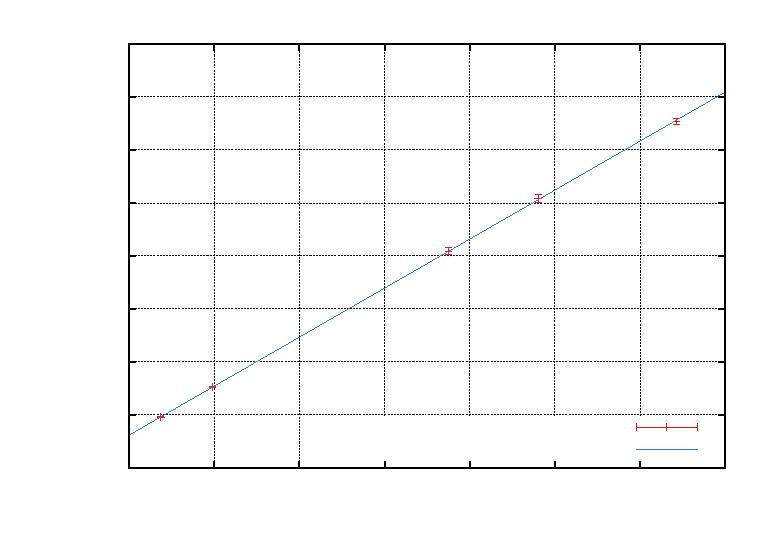
\includegraphics{./plots/planck_quantum_linearisierung}}%
    \gplfronttext
  \end{picture}%
\endgroup

	\caption{Linearisierung zur Bestimmung von $h$}
	\label{fig:lin_h}
\end{figure}
Zur Berechnung des Planckschen Wirkungsquantums wird die angepasste Gerade im Hinblick auf die Energiebilanz des Elektrons betrachtet.
Demnach ist die Steigung $m$ gegeben durch:
\begin{align*}
	m = \frac{h}{e}
\end{align*}
Das Wirkungsquantum wird durch Multiplikation der Steigung $m$ mit der Elementarladung \cite{CODATA}:
\begin{align}
	e = \SI{1.602176565 +- 0.000000035e-19}{\coulomb}
\end{align}
berechnet, wobei der Einfluss des Fehlers der Elementarladung klein gegen den der Steigung ist und daher vernachlässigt wird.
Somit ergibt sich:
\begin{align*}
	h = \SI{5.93 +- 0.04e-34}{\joule\second}
\end{align*}
Dieser Wert stimmt leider nicht mit dem Literaturwert $h = \SI{6.626 e-34}{\joule\second}$ \cite{CODATA} überein.
In Anbetracht des statistischen Fehlers muss hier von einem systematischen Fehler ausgegangen werden, dessen Ursache wir nicht eindeutig lokalisieren können.
In dieser Hinsicht liefert auch der Achsenabschnitt (auch unter Beachtung des Kontaktpotentials) keine gute Abschätzung für die Austrittsarbeit:
\begin{align*}
	W_\mathrm{K} + e \, U_\mathrm{Kontakt} = \SI{1.326 +- 0.008}{\electronvolt} \text{,}
\end{align*}
da diese für Kalium in der Größenordnung von $\SI{2.29}{\electronvolt}$ \cite{crc} liegen sollte.


\subsubsection{Einfluss der Intensität auf die Kennlinien}
\begin{figure}[h]
	\centering
	% GNUPLOT: LaTeX picture with Postscript
\begingroup
  \makeatletter
  \providecommand\color[2][]{%
    \GenericError{(gnuplot) \space\space\space\@spaces}{%
      Package color not loaded in conjunction with
      terminal option `colourtext'%
    }{See the gnuplot documentation for explanation.%
    }{Either use 'blacktext' in gnuplot or load the package
      color.sty in LaTeX.}%
    \renewcommand\color[2][]{}%
  }%
  \providecommand\includegraphics[2][]{%
    \GenericError{(gnuplot) \space\space\space\@spaces}{%
      Package graphicx or graphics not loaded%
    }{See the gnuplot documentation for explanation.%
    }{The gnuplot epslatex terminal needs graphicx.sty or graphics.sty.}%
    \renewcommand\includegraphics[2][]{}%
  }%
  \providecommand\rotatebox[2]{#2}%
  \@ifundefined{ifGPcolor}{%
    \newif\ifGPcolor
    \GPcolortrue
  }{}%
  \@ifundefined{ifGPblacktext}{%
    \newif\ifGPblacktext
    \GPblacktexttrue
  }{}%
  % define a \g@addto@macro without @ in the name:
  \let\gplgaddtomacro\g@addto@macro
  % define empty templates for all commands taking text:
  \gdef\gplbacktext{}%
  \gdef\gplfronttext{}%
  \makeatother
  \ifGPblacktext
    % no textcolor at all
    \def\colorrgb#1{}%
    \def\colorgray#1{}%
  \else
    % gray or color?
    \ifGPcolor
      \def\colorrgb#1{\color[rgb]{#1}}%
      \def\colorgray#1{\color[gray]{#1}}%
      \expandafter\def\csname LTw\endcsname{\color{white}}%
      \expandafter\def\csname LTb\endcsname{\color{black}}%
      \expandafter\def\csname LTa\endcsname{\color{black}}%
      \expandafter\def\csname LT0\endcsname{\color[rgb]{1,0,0}}%
      \expandafter\def\csname LT1\endcsname{\color[rgb]{0,1,0}}%
      \expandafter\def\csname LT2\endcsname{\color[rgb]{0,0,1}}%
      \expandafter\def\csname LT3\endcsname{\color[rgb]{1,0,1}}%
      \expandafter\def\csname LT4\endcsname{\color[rgb]{0,1,1}}%
      \expandafter\def\csname LT5\endcsname{\color[rgb]{1,1,0}}%
      \expandafter\def\csname LT6\endcsname{\color[rgb]{0,0,0}}%
      \expandafter\def\csname LT7\endcsname{\color[rgb]{1,0.3,0}}%
      \expandafter\def\csname LT8\endcsname{\color[rgb]{0.5,0.5,0.5}}%
    \else
      % gray
      \def\colorrgb#1{\color{black}}%
      \def\colorgray#1{\color[gray]{#1}}%
      \expandafter\def\csname LTw\endcsname{\color{white}}%
      \expandafter\def\csname LTb\endcsname{\color{black}}%
      \expandafter\def\csname LTa\endcsname{\color{black}}%
      \expandafter\def\csname LT0\endcsname{\color{black}}%
      \expandafter\def\csname LT1\endcsname{\color{black}}%
      \expandafter\def\csname LT2\endcsname{\color{black}}%
      \expandafter\def\csname LT3\endcsname{\color{black}}%
      \expandafter\def\csname LT4\endcsname{\color{black}}%
      \expandafter\def\csname LT5\endcsname{\color{black}}%
      \expandafter\def\csname LT6\endcsname{\color{black}}%
      \expandafter\def\csname LT7\endcsname{\color{black}}%
      \expandafter\def\csname LT8\endcsname{\color{black}}%
    \fi
  \fi
  \setlength{\unitlength}{0.0500bp}%
  \begin{picture}(6480.00,4320.00)%
    \gplgaddtomacro\gplbacktext{%
      \csname LTb\endcsname%
      \put(814,820){\makebox(0,0)[r]{\strut{} 0}}%
      \csname LTb\endcsname%
      \put(814,1467){\makebox(0,0)[r]{\strut{} 5}}%
      \csname LTb\endcsname%
      \put(814,2114){\makebox(0,0)[r]{\strut{} 10}}%
      \csname LTb\endcsname%
      \put(814,2761){\makebox(0,0)[r]{\strut{} 15}}%
      \csname LTb\endcsname%
      \put(814,3408){\makebox(0,0)[r]{\strut{} 20}}%
      \csname LTb\endcsname%
      \put(814,4055){\makebox(0,0)[r]{\strut{} 25}}%
      \csname LTb\endcsname%
      \put(1068,484){\makebox(0,0){\strut{} 0}}%
      \csname LTb\endcsname%
      \put(2291,484){\makebox(0,0){\strut{} 0,5}}%
      \csname LTb\endcsname%
      \put(3515,484){\makebox(0,0){\strut{} 1}}%
      \csname LTb\endcsname%
      \put(4738,484){\makebox(0,0){\strut{} 1,5}}%
      \csname LTb\endcsname%
      \put(5961,484){\makebox(0,0){\strut{} 2}}%
      \put(176,2379){\rotatebox{-270}{\makebox(0,0){\strut{}$I-I_0 \, / \, \si{\nano\ampere}$}}}%
      \put(3514,154){\makebox(0,0){\strut{}$U \, / \, \si{\volt}$}}%
      \put(3514,3945){\makebox(0,0){\strut{}}}%
    }%
    \gplgaddtomacro\gplfronttext{%
      \csname LTb\endcsname%
      \put(5096,3882){\makebox(0,0)[r]{\strut{}Messung 1}}%
      \csname LTb\endcsname%
      \put(5096,3662){\makebox(0,0)[r]{\strut{}Messung 2}}%
    }%
    \gplbacktext
    \put(0,0){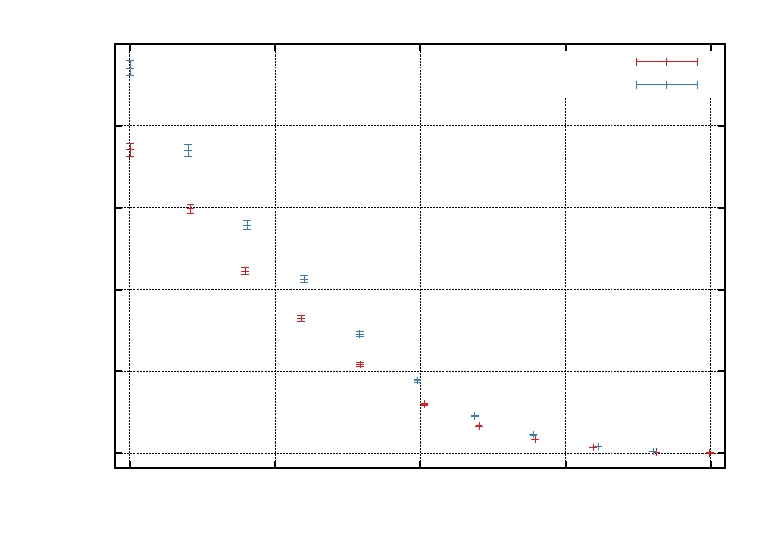
\includegraphics{./plots/kennlinie_intensitaet}}%
    \gplfronttext
  \end{picture}%
\endgroup

	\caption{Intensitätsvergleich der Kennlinien $\lambda = \SI{365}{\nano\metre}$}
	\label{fig:kennlinie_intensitaet}
\end{figure}
Bei der Durchführung wurde die Kennlinie der Photozelle bei der Wellenlänge $\lambda = \SI{365}{\nano\metre}$ jeweils bei zwei unterschiedlichen Intensitäten gemessen.
In Abbildung \ref{fig:kennlinie_intensitaet} wurden beide Kennlinien aufgetragen und im Folgenden soll deren Charakteristika diskutiert werden.
Zunächst erkennt man eine signifikante Abweichung der Kathodenphotoströme, welche mit steigender Gegenspannung $U$ sinkt und schließlich bei der gleichen Grenzfrequenz $U_0$ verschwindet.
Dies ist nicht verwunderlich, denn wie schon in Abschnitt \ref{ssec:photoeffekt} besprochen, hängt die Energie des Elektrons nur von der Frequenz des Photons ab und nicht von der Intensität des einfallenden Lichts.
Daher kommt es auch zu einem Verschwinden des Photostroms bei derselben Gegenspannung, was in den beiden Kennlinien gut sichtbar ist.
\clearpage
\section{Balmer-Serie}

\subsection{Durchführung}

\subsubsection{Aufbau und Justage}
\label{sssec:balmer_okular}
\begin{figure}[h]
\centering
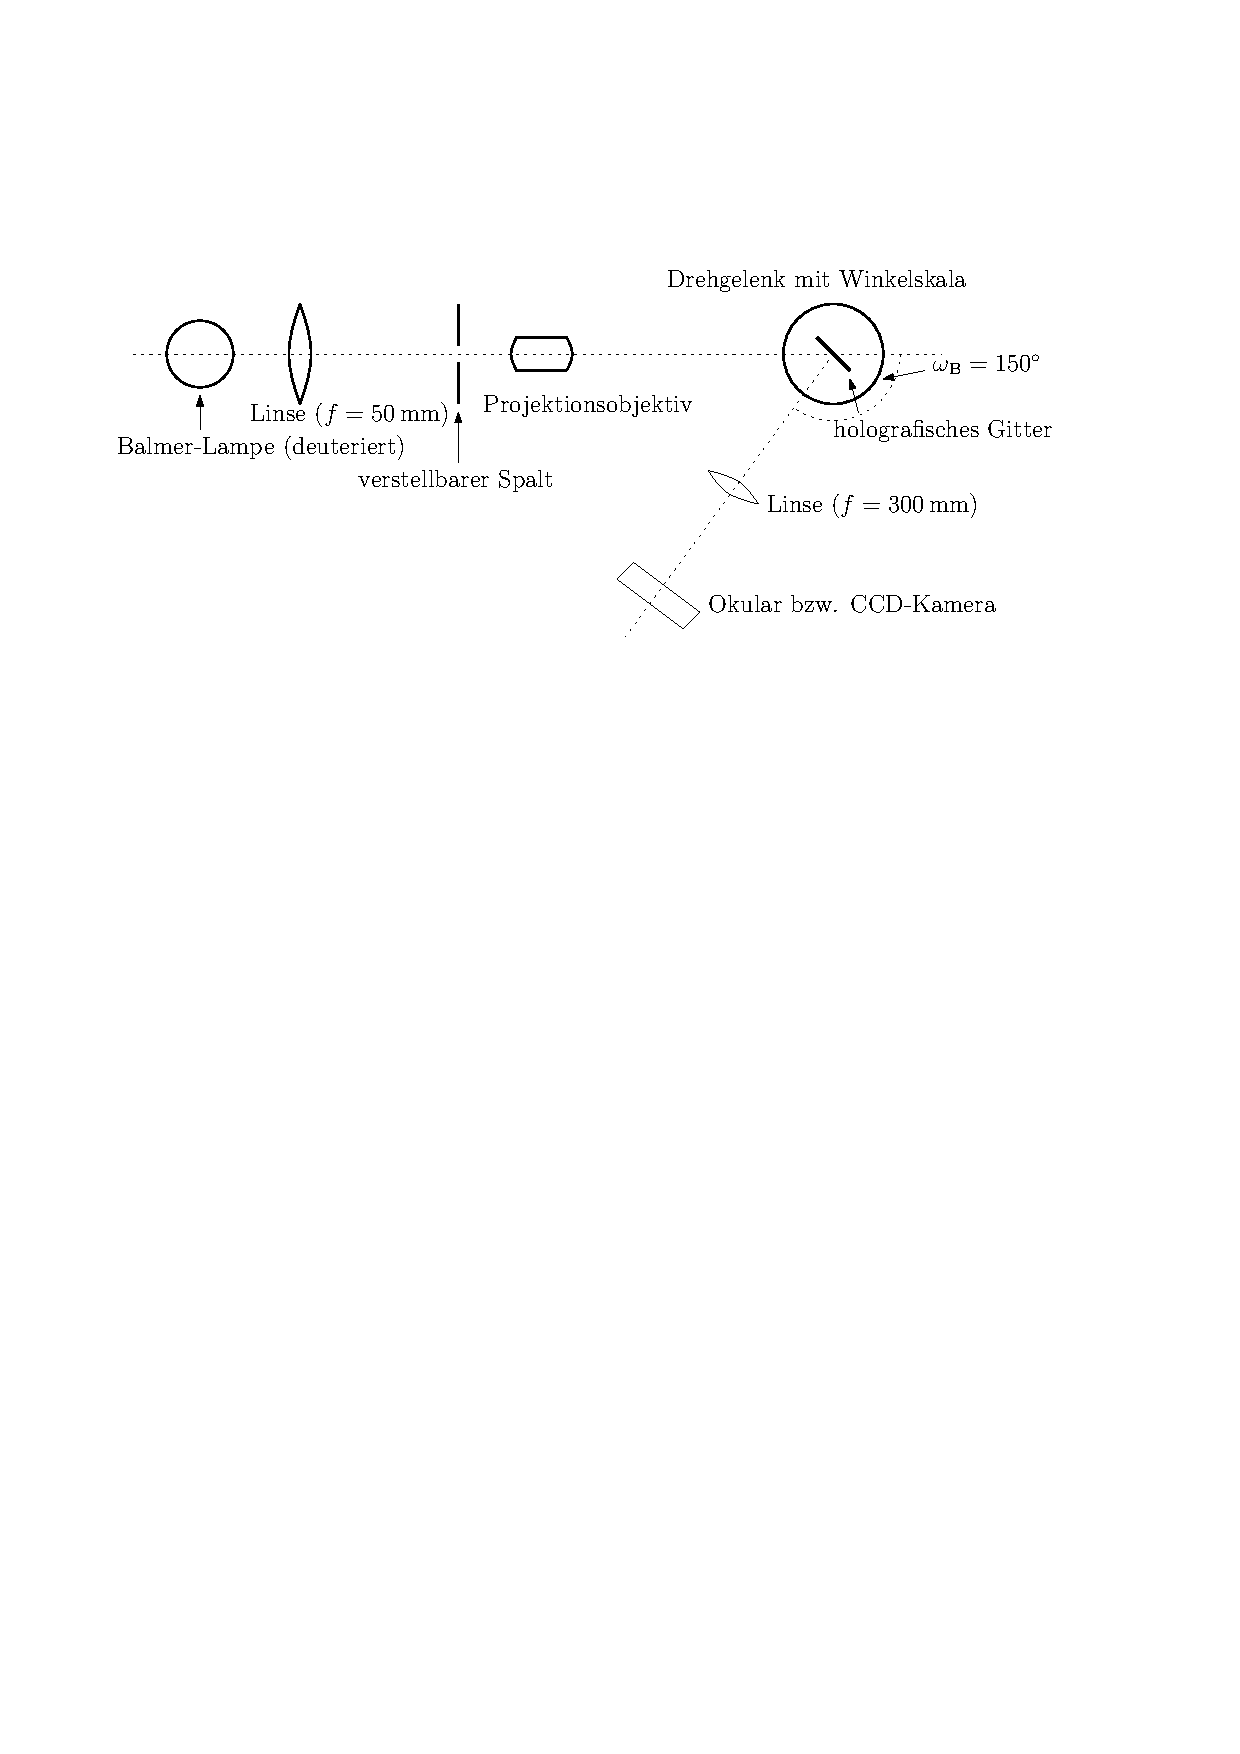
\includegraphics[width=\textwidth]{./figures/versuchsaufbau_balmerserie.pdf}
\caption{Versuchsanordnung zur Beobachtung der Balmer-Serie mit Okular bzw. CCD-Kamera}
\label{fig:aufbau_balmer}
\end{figure}
\noindent Der Versuchsaufbau erfolgt wie in Abbildung \ref{fig:aufbau_balmer} gezeigt.
Dabei wird der Aufbau zunächst mit einer Quecksilber-Spektrallampe justiert, da die Intensität dort höher ist.
Auf der ersten optischen Bank werden Linse, Spalt und Projektionsobjektiv befestigt.
Mit den Reflexen des Lichts am auf \SI{0}{\degree} gedrehten Gitter kann eine möglichst genaue Ausrichtung aller Elemente entlang einer optischen Achse sichergestellt werden.
Die Linse mit \SI{50}{\milli\metre} Brennweite wird dabei so positioniert, dass sie die Lampe scharf auf den Spalt abbildet.
Nun wird direkt neben dem Spalt durch Reflexion am Gitter eine scharfe Abbildung des Spalts selbst erreicht, in dem das Projektionsobjektiv zunächst grob positioniert und durch Drehen an der Linse optimal eingestellt wird.
Der Aufbau befindet sich danach in so genannter Autokollimation, was bedeutet, dass der Spalt ins Unendliche abgebildet wird.
Die zweite optische Bank wird so gedreht, dass sie mit der ersten optischen Bank einen Bankwinkel $\omega_\text{B}$ zwischen \SI{130}{\degree} und \SI{170}{\degree} bildet.
Für die Durchführung wird $\omega_\text{B}$=\SI{150 +- 0.25}{\degree} gewählt und  für alle Versuchsteile beibehalten und vor den Messungen kontrolliert und gegebenenfalls neu justiert.
Am Ende der zweiten optischen Bank wird das Okular befestigt und so eingestellt, dass die Skala gut ablesbar ist.
Mit Hilfe der Linse mit \SI{300}{\milli\metre} Brennweite kann das zu beobachtende Spektrum scharf auf das Okular abgebildet werden (Fernrohraufbau).

\subsubsection{Bestimmung der Gitterkonstanten}
\label{sssec:durchfuehrung_gitterkonstante}
Die Bestimmung der Gitterkonstante erfolgt mit einer Hg-Spektrallampe, da sie viele beobachtbare Linien hat und so eine gute Messung mit möglichst vielen Werten möglich ist.
Dazu wird das Gitter während ständiger Beobachtung durch das Okular so gedreht, bis die erste sichtbare Linie erscheint.
Hierfür sollte der Spalt zunächst weit geöffnet sein, um eine hohe Intensität zu erreichen und nach Auffinden der Linie verkleinert werden, um eine möglichst genaue Messung durchzuführen.
Ist die entsprechende Linie mit der Linse mit Brennweite $f=\SI{300}{\milli\metre}$ scharf im Okular zu beobachten wird der Gitterwinkel $\omega_\text{G}$ auf der Winkelskala abgelesen.
Hier ist abermals darauf zu achten, dass der Bankwinkel weiterhin \SI{150}{\degree} beträgt.
So verfährt man für alle sichtbaren Linien, die im Anschluss an die Messung mit Hilfe der gegebenen Tabelle der sichtbaren Spektrallinien von Quecksilber einer Wellenlänge zugeordnet werden können.
Da manche Linien dicht beieinander lagen, wurde deren relative Position $d$ zum Zentrum des Okulars an der Strichskala abgelesen.
Die entsprechenden Messwerte sind in Tabelle \ref{tab:gitterkonstante_messdaten} notiert.
\begin{table}[h]
	\centering
	\begin{tabular}{SSS}
	\toprule
	{$\lambda$ / \si{\nano\metre}} & {$\omega_\mathrm{G}$ / \si{\degree}} & {$d$ / \si{\milli\metre}}\\
	\midrule
	404.656 & 46.0 & 2.10  \\
	407.783 & 46.0 & 0.00  \\
	410.805 & 46.0 & -2.10 \\
	\midrule
	433.922 & 48.5 & 1.30  \\
	434.749 & 48.5 & 0.70  \\
	435.833 & 48.5 & 0.00  \\
	\midrule
	491.607 & 53.5 & 0.00  \\
	\midrule
	546.074 & 58.5 & 0.00  \\
	\midrule
	576.960 & 62.0 & 1.70  \\
	579.066 & 62.0 & 0.00  \\
	\midrule
	623.440 & 67.0 & 0.00  \\
	\midrule
	671.643 & 72.5 & 0.00 \\
	\bottomrule
\end{tabular}

	\caption{Lage der Quecksilber Linien bei der Messung mit dem Reflektionsgitter. $d$ kennzeichnet die Lage der Linie auf der Strichskala des Okulars bei gegebenem Gitterwinkel und entspricht für $d = \SI{0}{\milli\metre}$ dem Zentrum der Skala. Fehler: $\Delta \omega_\mathrm{G} = \SI{0.5}{\degree}$, $\Delta d = \SI{0.05}{\milli\metre}$}
	\label{tab:gitterkonstante_messdaten}
\end{table}

\subsubsection{Messung der Balmer-Linien mit einem Okular} 
Zu den weiteren Messungen wird nun die Quecksilberlampe gegen eine deuterierte Balmer-Lampe getauscht (Mischungsverhältnis ca. 1:2).
Wie bei der Bestimmung der Gitterkonstante dreht man nun das Gitter bis man eine beobachtbare Wasserstofflinie (hellere der beiden Linien) sieht und notiert den Gitterwinkel $\omega_\text{G}$, bei dem die Linie im Nullpunkt der Okularskala liegt.
Hieraus kann später die Wellenlänge der beobachteten Linie gemessen werden.
Außerdem wird wie oben die Verschiebung $d$ notiert, unter der die Deuteriumlinie (schwächere der beiden Linien) im Okular auftritt, um so später die Isotopieaufspaltung zu bestimmen.
Die Messdaten wurden in Tabelle \ref{tab:balmer_okular_messdaten} aufgetragen.
\begin{table}[h]
	\centering
	\begin{tabular}{lSS}
\toprule
{Linie}   & {Gitterwinkel $\omega_\mathrm{G}$ / \si{\degree}} & {Aufspaltung $d$ / \si{\milli\metre}}\\
\midrule
H$\alpha$     & 70.5 +- 0.5      & 0.18 +- 0.02        \\
H$\beta$      & 53 +- 0.5        & 0.10 +- 0.02        \\
H$\gamma$     & 48 +- 0.5        & 0.08 +- 0.02        \\
H$\delta$     & 46 +- 0.5        &                     \\ 
\bottomrule
\end{tabular}
	\caption{Messdaten der mit dem Okular bestimmten Balmer-Linien}
	\label{tab:balmer_okular_messdaten}
\end{table}

\subsubsection{Messung der Balmer-Linien mit einer CCD-Kamera}
Es wird der Versuchsaufbau wie in \ref{sssec:balmer_okular} beschrieben genutzt, allerdings mit einer CCD-Kamera anstelle des Okulars. 
Im Programm VideoCom wird die Brennweite der auf die CCD-Zeile abbildenden Linse (\SI{300}{\milli\meter}) eingetragen, so dass jedem der 2048 Pixel ein Winkel zugeordnet werden kann, der im folgenden mit $\delta$ bezeichnet wird.
Um die Linien aufzufinden wird das Okular auf einem zusätzlichen Reiter aufgebaut (um die vertikale Ausrichtung bei jedem Durchgang nicht anpassen zu müssen) und das Gitter entsprechend gedreht, bis die Linie möglichst zentral liegt.
Die CCD-Kamera wird nun statt des Okulars auf der optischen Bank aufgebaut und das Intensitätsprofil kann auf dem Bildschirm betrachtet werden, um die Abbildungslinse so zu verschieben, bis sie scharf auf die Kamera abbildet.
Durch Vergrößerung des Bildschausschnitts kann der Bereich der Linie besser betrachtet werden können und die Spaltbreite wird so angepasst, dass eine möglichst hohe Intensität und gleichzeitig eine gute Aufspaltung erreicht wird.
Da dies nicht immer eindeutig gelang wurden zu jeder Linie mehrere Messungen durchgeführt und zur Auswertung jeweils die Messung gewählt, bei der die Aufspaltung gut zu erkennen war.
Wegen der teilweise hohen Schwankungen der Intensität lässt man die Messwerte im Programm über eine gewisse Zeit mitteln, bis mit dem Auge beinahe keine Schwankungen mehr zu erkennen sind.

\subsection{Auswertung}

\subsubsection{Bestimmung der Gitterkonstanten}
\label{sssec:gitterkonstante}
\begin{figure}[h]
	\centering
	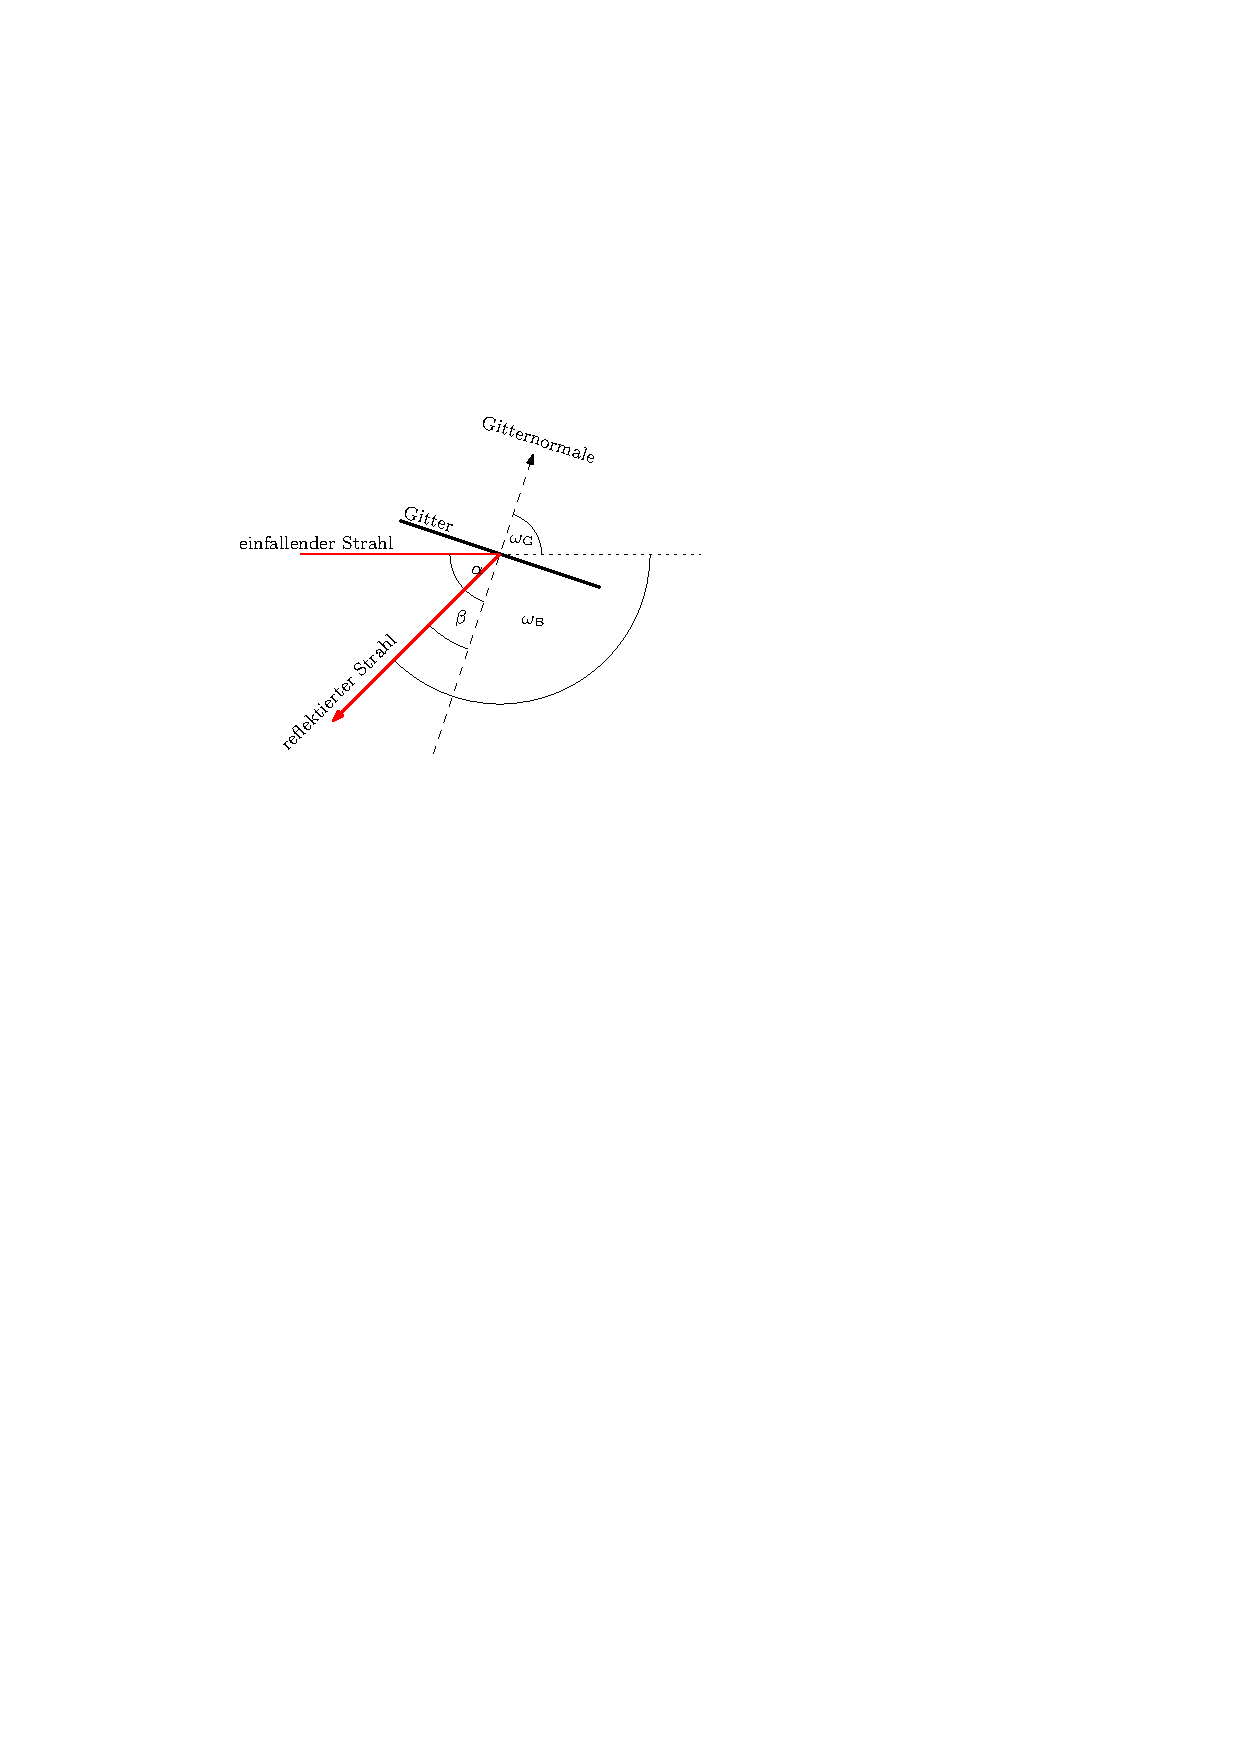
\includegraphics[width=0.65\textwidth]{./figures/winkelverhaeltniss.pdf}
	\caption{Winkelverhältnis zwischen Gitter und optischer Bank}
	\label{fig:winkelverhaeltnis}
\end{figure}
Aus Abbildung \ref{fig:winkelverhaeltnis} folgt der Zusammenhang zwischen den gemessenen Winkeln ($\omega_\mathrm{G}$, $\omega_\mathrm{B}$) und den Ein- beziehungsweise Ausfallswinkeln des Strahls auf das Gitter ($\alpha$, $\beta$): 
\begin{align*}
	\alpha &= \omega_\text{G} \\
	\beta &= \omega_\text{G} + \omega_\text{B} - \SI{180}{\degree}
	\label{eq:reflexionswinkel}
\end{align*}
Da nahe beieinanderliegende Linien nicht durch Verstellen des Gitters zu messen waren und stattdessen die Abweichung vom Zentrum des Okulars $d$ auf der darin angebrachten Skala abgelesen wurde, muss eine Korrektur des Ausfallswinkels anhand der gemessenen Abweichung $d$ erfolgen.
Diese ist (in Kleinwinkelnäherung) gegeben durch die Brennweite $f$ des Objektivs im Fernrohraufbau:
\begin{align*}
\Delta \beta = -\frac{d}{f} \text{,}
\end{align*}
wobei das Vorzeichen von der Messrichtung von $d$ abhängt.
Hier wurde $d$ so gemessen, dass es rechts vom Zentrum der Strichskala positiv ist und somit kleineren Ausfallswinkeln $\beta$ entspricht.
Mit der Brennweite des Fernrohrobjektivs $f = \SI{300}{\milli\metre}$ folgt mit der erwähnten Korrektur für den tatsächlichen Ausfallswinkel:
\begin{align*}
	\beta^\prime = \beta + \Delta \beta
\end{align*}
Die Berechnung der Winkel erfolgt nun über die gemessenen Winkel und deren Fehler aus Tabelle \ref{tab:gitterkonstante_messdaten}, wobei für den Bankwinkel $\omega_\mathrm{B} = \SI{150 +- 0.25}{\degree}$ gilt.
Dabei überträgt sich der Fehler der Winkelmessung des Gitters direkt auf den Einfallswinkel $\alpha$ und die Fehler in $\omega_\mathrm{G}$, $\omega_\mathrm{B}$ und $\Delta \beta$ auf den Ausfallswinkel $\beta$ durch die Wurzel der quadratischen Addition der Fehler (um Verwechslung mit $\Delta \beta$ zu vermeiden werden die Fehler hier durch $\sigma$ gekennzeichnet):
\begin{align*}
	\sigma_\beta = \sqrt{\sigma_{\omega_\mathrm{G}}^2 + \sigma_{\omega_\mathrm{B}}^2 + \left(\frac{\sigma_d}{f}\right)^2}
\end{align*}
Wegen $\sigma_{\omega_\mathrm{G}} = \SI{0.25}{\degree}$, $\sigma_{\omega_\mathrm{B}} = \SI{0.5}{\degree}$ und $\sigma_d = \SI{0.05}{\milli\metre}$ folgt für die Fehler:
\begin{align*}
	\sigma_\alpha = \SI{8.8}{\milli\radian}\\
	\sigma_\beta = \SI{9.8}{\milli\radian}
\end{align*}
und sind somit unabhängig von der Messung.
Die berechneten Winkel wurde in Tabelle \ref{tab:gitterkonstante_umrechnung_winkel} zusammengetragen.
\begin{table}[h]
	\centering
	\begin{tabular}{SSS}
	\toprule
	{$\lambda$ / \si{\nano\metre}} & {$\alpha$ / \si{\milli\radian}} & {$\beta$ / \si{\milli\radian}}\\
	\midrule
	404.656     & 802.9        & 272.3       \\
	407.783     & 802.9        & 279.3       \\
	410.805     & 802.9        & 286.3       \\
	433.922     & 846.5        & 318.6       \\
	434.749     & 846.5        & 320.6       \\
	435.833     & 846.5        & 322.9       \\
	491.607     & 933.8        & 410.2       \\
	546.074     & 1021.0       & 497.4       \\
	576.960     & 1082.1       & 552.8       \\
	579.066     & 1082.1       & 558.5       \\
	623.440     & 1169.4       & 645.8       \\
	671.643     & 1265.4       & 741.8  	 \\
	\bottomrule
\end{tabular}

	\caption{Ergebnisse der Umrechnung $\Delta \alpha = \SI{8.8}{\milli\radian}$ und $\Delta \beta = \SI{9.8}{\milli\radian}$}
	\label{tab:gitterkonstante_umrechnung_winkel}
\end{table}

Nachdem die gemessenen Winkel in Ein- und Ausfallswinkel am Gitter umgerechnet wurden, kann mithilfe der Gittergleichung in erster Interferenzordnung:
\begin{align}
	\lambda = g \cdot (\sin(\alpha) + \sin(\beta))
\end{align}
die Gitterkonstante $g$ bestimmt werden.
Dazu tragen wir $\sin(\alpha) + \sin(\beta)$ gegen die Wellenlänge $\lambda$ auf, um:
\begin{align*}
\sin(\alpha) + \sin(\beta) = \frac{1}{g} \cdot \lambda
\end{align*}
zu erhalten.
Diese Form der Linearisierung wird gewählt, da bei einer Anpassung mit üblichen Least-Squares-Verfahren nur die Fehler in $y$-Richtung in die Gewichtung der Messpunkte eingehen.
Da der Fehler der Wellenlänge $\lambda$ gegen den der Sinus-Summe vernachlässigbar ist, wurde diese Form gewählt um eine sinnvolle Gewichtung bei der Geradenanpassung zu erzielen.
Mithilfe von \texttt{Gnuplot} wird eine Ursprungsgerade an die linearisierten Datenpunkte angepasst.
Dabei wird der Fehler der Sinus-Summe gemäß Gaußsscher Fehlerfortpflanzung in den Größen $\alpha$ und $\beta$ berechnet.
Die Anpassung ergibt:
\begin{align}
	\sin(\alpha) + \sin(\beta) = \SI{2439.6 +- 2.1}{\per\milli\metre} \cdot \lambda \text{,}
\end{align}
bei einem reduzierten Chi-Quadrat von $\chi_\mathrm{red.}^2 = \num{1.3e-5}$.
In Anbetracht des Chi-Quadrates liegt eine gute Anpassung vor, dennoch scheinen die Datenpunkte besser auf einer Geraden zu liegen als deren Fehler nahelegen.
Auch die Tatsache, dass $\chi_\mathrm{red.}^2 \ll 1$ legt nahe, dass die statistischen Fehler der Winkelmessungen überschätzt wurden.
In Abbildung \ref{fig:gitterkonstante} wurden die Datenpunkte mitsamt Regressionsgerade aufgetragen.
\begin{figure}[h]
	\centering
	% GNUPLOT: LaTeX picture with Postscript
\begingroup
  \makeatletter
  \providecommand\color[2][]{%
    \GenericError{(gnuplot) \space\space\space\@spaces}{%
      Package color not loaded in conjunction with
      terminal option `colourtext'%
    }{See the gnuplot documentation for explanation.%
    }{Either use 'blacktext' in gnuplot or load the package
      color.sty in LaTeX.}%
    \renewcommand\color[2][]{}%
  }%
  \providecommand\includegraphics[2][]{%
    \GenericError{(gnuplot) \space\space\space\@spaces}{%
      Package graphicx or graphics not loaded%
    }{See the gnuplot documentation for explanation.%
    }{The gnuplot epslatex terminal needs graphicx.sty or graphics.sty.}%
    \renewcommand\includegraphics[2][]{}%
  }%
  \providecommand\rotatebox[2]{#2}%
  \@ifundefined{ifGPcolor}{%
    \newif\ifGPcolor
    \GPcolortrue
  }{}%
  \@ifundefined{ifGPblacktext}{%
    \newif\ifGPblacktext
    \GPblacktexttrue
  }{}%
  % define a \g@addto@macro without @ in the name:
  \let\gplgaddtomacro\g@addto@macro
  % define empty templates for all commands taking text:
  \gdef\gplbacktext{}%
  \gdef\gplfronttext{}%
  \makeatother
  \ifGPblacktext
    % no textcolor at all
    \def\colorrgb#1{}%
    \def\colorgray#1{}%
  \else
    % gray or color?
    \ifGPcolor
      \def\colorrgb#1{\color[rgb]{#1}}%
      \def\colorgray#1{\color[gray]{#1}}%
      \expandafter\def\csname LTw\endcsname{\color{white}}%
      \expandafter\def\csname LTb\endcsname{\color{black}}%
      \expandafter\def\csname LTa\endcsname{\color{black}}%
      \expandafter\def\csname LT0\endcsname{\color[rgb]{1,0,0}}%
      \expandafter\def\csname LT1\endcsname{\color[rgb]{0,1,0}}%
      \expandafter\def\csname LT2\endcsname{\color[rgb]{0,0,1}}%
      \expandafter\def\csname LT3\endcsname{\color[rgb]{1,0,1}}%
      \expandafter\def\csname LT4\endcsname{\color[rgb]{0,1,1}}%
      \expandafter\def\csname LT5\endcsname{\color[rgb]{1,1,0}}%
      \expandafter\def\csname LT6\endcsname{\color[rgb]{0,0,0}}%
      \expandafter\def\csname LT7\endcsname{\color[rgb]{1,0.3,0}}%
      \expandafter\def\csname LT8\endcsname{\color[rgb]{0.5,0.5,0.5}}%
    \else
      % gray
      \def\colorrgb#1{\color{black}}%
      \def\colorgray#1{\color[gray]{#1}}%
      \expandafter\def\csname LTw\endcsname{\color{white}}%
      \expandafter\def\csname LTb\endcsname{\color{black}}%
      \expandafter\def\csname LTa\endcsname{\color{black}}%
      \expandafter\def\csname LT0\endcsname{\color{black}}%
      \expandafter\def\csname LT1\endcsname{\color{black}}%
      \expandafter\def\csname LT2\endcsname{\color{black}}%
      \expandafter\def\csname LT3\endcsname{\color{black}}%
      \expandafter\def\csname LT4\endcsname{\color{black}}%
      \expandafter\def\csname LT5\endcsname{\color{black}}%
      \expandafter\def\csname LT6\endcsname{\color{black}}%
      \expandafter\def\csname LT7\endcsname{\color{black}}%
      \expandafter\def\csname LT8\endcsname{\color{black}}%
    \fi
  \fi
  \setlength{\unitlength}{0.0500bp}%
  \begin{picture}(7200.00,5040.00)%
    \gplgaddtomacro\gplbacktext{%
      \csname LTb\endcsname%
      \put(946,704){\makebox(0,0)[r]{\strut{} 400}}%
      \csname LTb\endcsname%
      \put(946,1383){\makebox(0,0)[r]{\strut{} 450}}%
      \csname LTb\endcsname%
      \put(946,2061){\makebox(0,0)[r]{\strut{} 500}}%
      \csname LTb\endcsname%
      \put(946,2740){\makebox(0,0)[r]{\strut{} 550}}%
      \csname LTb\endcsname%
      \put(946,3418){\makebox(0,0)[r]{\strut{} 600}}%
      \csname LTb\endcsname%
      \put(946,4097){\makebox(0,0)[r]{\strut{} 650}}%
      \csname LTb\endcsname%
      \put(946,4775){\makebox(0,0)[r]{\strut{} 700}}%
      \csname LTb\endcsname%
      \put(1078,484){\makebox(0,0){\strut{} 0.9}}%
      \csname LTb\endcsname%
      \put(1794,484){\makebox(0,0){\strut{} 1}}%
      \csname LTb\endcsname%
      \put(2509,484){\makebox(0,0){\strut{} 1.1}}%
      \csname LTb\endcsname%
      \put(3225,484){\makebox(0,0){\strut{} 1.2}}%
      \csname LTb\endcsname%
      \put(3941,484){\makebox(0,0){\strut{} 1.3}}%
      \csname LTb\endcsname%
      \put(4656,484){\makebox(0,0){\strut{} 1.4}}%
      \csname LTb\endcsname%
      \put(5372,484){\makebox(0,0){\strut{} 1.5}}%
      \csname LTb\endcsname%
      \put(6087,484){\makebox(0,0){\strut{} 1.6}}%
      \csname LTb\endcsname%
      \put(6803,484){\makebox(0,0){\strut{} 1.7}}%
      \put(176,2739){\rotatebox{-270}{\makebox(0,0){\strut{}Wellenlänge $\lambda$ / \si{\nano\meter}}}}%
      \put(3940,154){\makebox(0,0){\strut{}$\sin(\alpha)+\sin(\beta)$'}}%
      \put(3940,4665){\makebox(0,0){\strut{}}}%
    }%
    \gplgaddtomacro\gplfronttext{%
      \csname LTb\endcsname%
      \put(5816,1097){\makebox(0,0)[r]{\strut{}Messwerte}}%
      \csname LTb\endcsname%
      \put(5816,877){\makebox(0,0)[r]{\strut{}Regressionsgerade}}%
    }%
    \gplbacktext
    \put(0,0){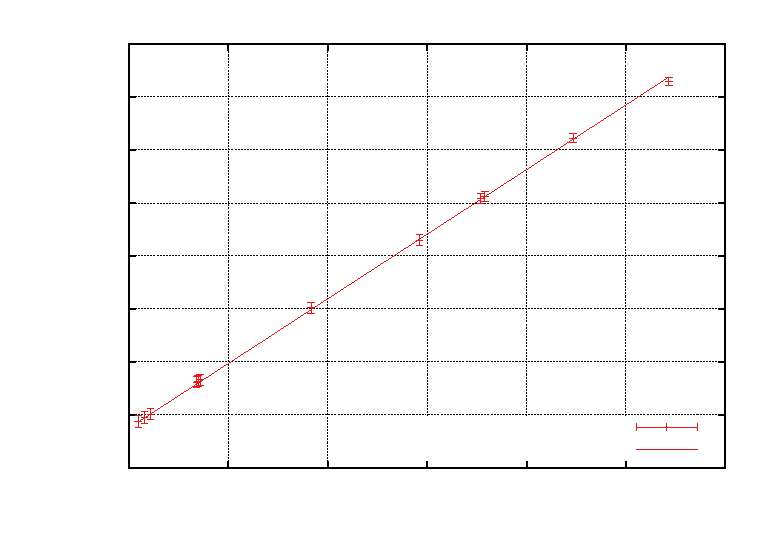
\includegraphics{./plots/gitterkonstante}}%
    \gplfronttext
  \end{picture}%
\endgroup

	\caption{Gitterkonstante}
	\label{fig:gitterkonstante}
\end{figure}
An der Steigung der Geraden lässt sich sofort die Gitterkonstanten in reziproken Einheiten ablesen, sodass man:
\begin{align*}
	\frac{1}{g} = (\num{2439.6 +- 2.1}) \, \frac{\mathrm{Linien}}{\si{\milli\metre}}
\end{align*}
erhält. Nach Kehrwertbildung ergibt sich:
\begin{align*}
	g = \SI{409.90 +- 0.36}{\nano\metre} \text{,}
\end{align*}
wobei der Fehler $\Delta g$ gegeben ist durch:
\begin{align*}
	\Delta g = \frac{\Delta \left( \frac{1}{g} \right)}{\left( \frac{1}{g} \right)^2} \text{.}
\end{align*}

\subsubsection{Wellenlängen und Isotopieaufspaltung der Balmer-Linien bei Beobachtung mit dem Okular}
\label{sssec:balmer_okular_aufspaltung}
\begin{table}[h]
	\centering
	\begin{tabular}{lSS}
\toprule
&\multicolumn{2}{c}{Wellenlänge}\\ \cmidrule(l){2-3}
{Linie} & {$\lambda$ / \si{\nano\metre}} & {$\lambda_\mathrm{Lit.}$ / \si{\nano\metre}}\\
\midrule
H$_\alpha$     & 652.6 +- 3.4 & 656.3 \\
H$_\beta$      & 487.5 +- 4.3 & 486.1 \\
H$_\gamma$     & 431.3 +- 4.6 & 434.0 \\
H$_\delta$     & 407.8 +- 4.6 & 410.2 \\ 
\bottomrule
\end{tabular}
	\caption{Berechnete Wellenlängen der Balmer-Linien. Literaturwerte aus \emph{NIST Atomic Spectra Database} \cite{NISTSpectra}}
	\label{tab:balmer_wellenlaenge}
\end{table}
Da die Gitterkonstante anhand des Quecksilberspektrums bestimmt wurde, ist es nun möglich die Wellenlängen der beobachteten Balmer-Linien mit der Gittergleichung zu bestimmen.
Es werden auch hier Interferenzordnungen erster Ordnung vermessen, sodass die Wellenlänge berechnet werden kann durch:
\begin{align*}
  \lambda = g \cdot ( \sin(\alpha) + \sin(\beta)) \text{.}
\end{align*}
Die Ein- und Ausfallswinkel werden dabei analog zu Abschnitt \ref{sssec:gitterkonstante} aus den gemessenen Gitter- und Bankwinkeln in Tabelle \ref{tab:balmer_okular_messdaten} (hier jedoch ohne Korrektur, da bei der Messung die Strichskala auf die Wasserstoff-Linie zentriert wurde).
Unter Beachtung der Fehler der Winkel $\alpha$, $\beta$ sowie der gemessenen Gitterkonstante $g = \SI{409.90 +- 0.36}{\nano\metre}$ ergeben sich die Wellenlängen aus Tabelle \ref{tab:balmer_wellenlaenge}.

Um die Isotopieaufspaltung zu bestimmen, misst man die Aufspaltung im Okular $d$.
Die Umrechnung der Aufspaltung im Okular in eine Aufspaltung des Ausfallwinkels $\Delta \beta$, wie zuvor bei der Winkelkorrektur bei der Bestimmung der Gitterkonstanten, ist durch die Brennweite des Fernrohrobjektivs $f$ in Kleinwinkelnäherung gegeben:
\begin{align*}
  \Delta \beta = \frac{d}{f}
\end{align*}
Um dies in eine Wellenlängenaufspaltung $\Delta \lambda$ umzurechnen, betrachtet man das Differential der Gittergleichung in erster Ordnung:
\begin{align*}
  \mathrm{d}\lambda = \frac{\partial \lambda}{\partial \alpha} \mathrm{d}\alpha + \frac{\partial \lambda}{\partial \beta} \mathrm{d}\beta
\end{align*}
In linearer Approximation ($\Delta \alpha = \num{0}$) folgt somit:
\begin{align}
  \Delta \lambda &= \frac{\partial \lambda}{\partial \beta} \cdot \Delta \beta \\
  &= g \cos(\beta) \Delta \beta \text{,}
  \label{eq:gitter_differenzial}
\end{align}
wobei der Fehler mittels Gaußsscher Fehlerfortpflanzung zu:
\begin{align*}
	\sigma_{\Delta \lambda} = \sqrt{\left( \cos(\beta) \Delta \beta \cdot \sigma_g \right)^2 + \left( g \cdot \sin(\beta) \Delta \beta \cdot \sigma_\beta \right)^2 + \left( g \cdot \cos(\beta) \cdot \sigma_{\Delta \beta}\right)^2}
\end{align*}
bestimmt wurde mit
\begin{align*}
	\sigma_\beta &= \sqrt{\sigma_{\omega_\mathrm{G}}^2 + \sigma_{\omega_\mathrm{B}}^2} \\
	\sigma_{\Delta \beta} &= \frac{\sigma_d}{f}
\end{align*}
und $\sigma_g$ aus der Bestimmung der Gitterkonstante.
Die Berechnung der Isotopieaufspaltung anhand der Beobachtung mit dem Okular und Vergleich mit den theoretischen Werten wurde in Tabelle \ref{tab:balmer_aufspaltung_okular} aufgetragen.
\begin{table}[h]
	\centering
	\begin{tabular}{lSS}
	\toprule
	&\multicolumn{2}{c}{Isotopieaufspaltung}\\ \cmidrule(l){2-3}
	{Linie} & {$\Delta \lambda$ / \si{\pico\metre}} & {$\Delta \lambda_\mathrm{theo.}$ / \si{\pico\metre}}\\
	\midrule
	H$\alpha$     & 187.0 +- 20.9 & 178.8 \\
	H$\beta$      & 125.8 +- 25.2 & 132.4 \\
	H$\gamma$     & 104.0 +- 26.0 & 118.2 \\
	H$\delta$     &  & 111.7 \\ 
	\bottomrule
\end{tabular}
	\caption{Berechnete Isotopieaufspaltung mit dem Okular. Theoretische Werte wurden mithilfe der Rydberg-Formel aus Abschnitt \ref{sssec:rydberg} und den physikalischen Konstanten von \cite{CODATA} berechnet.}
	\label{tab:balmer_aufspaltung_okular}
\end{table}
In Anbetracht der Fehler stimmen die hier berechneten Werte für die Isotopieaufspaltung gut mit den theoretischen überein.

\subsubsection{Bestimmung der Rydberg-Konstanten aus den Linien der Balmer-Serie}
Da die Wellenlängen der ersten vier Linien der Balmer-Serie bestimmt wurden, kann nun mithilfe der Rydberg-Formel (ref Theorieteil) und einer geeigneten Linearisierung eine Bestimmung der Rydberg-Konstanten durchgeführt werden.
Konkret liefert die Rydberg-Formel für die Balmer-Serie (Übergang: $n \rightarrow 2$) von Wasserstoff:
\begin{align*}
	\frac{1}{\lambda} = R_\mathrm{H} \cdot \left(\frac{1}{2^2} - \frac{1}{n^2} \right) \text{,}
\end{align*}
wobei die Linien H$_\alpha$, H$_\beta$, H$_\gamma$, H$_\delta$ den natürlichen Zahlen $n = 3, 4, 5, 6$ entsprechen.
Zur Linearisierung kann nun $\frac{1}{\lambda}$ gegen $\frac{1}{4} - \frac{1}{n^2}$ aufgetragen werden.
Dazu wurde in Tabelle \ref{tab:rydberg_linearisierung} die reziproke Wellenlänge gebildet und deren Fehler mit Gaußsscher Fehlerfortpflanzung berechnet.
\begin{table}[h]
	\centering
	\begin{tabular}
{	l
	S[table-parse-only]
	S
}
\toprule
{Linie} & n & {$\lambda^{-1}$ / \si{\per\micro\metre}}\\
\midrule
H$\alpha$     & 3 & 1.532 +- 0.008 \\
H$\beta$      & 4 & 2.051 +- 0.019 \\
H$\gamma$     & 5 & 2.319 +- 0.025 \\
H$\delta$     & 6 & 2.452 +- 0.028 \\ 
\bottomrule
\end{tabular}
	\caption{Linearisierte Werte für Rydberg}
	\label{tab:rydberg_linearisierung}
\end{table}
Es wird folglich eine Ursprungsgerade mit \texttt{Gnuplot} an die linearisierten Datenpunkte angepasst, welche zusammen in Abbildung \ref{fig:rydberg_balmer} aufgetragen sind.
\begin{figure}[h]
	\centering
	% GNUPLOT: LaTeX picture with Postscript
\begingroup
  \makeatletter
  \providecommand\color[2][]{%
    \GenericError{(gnuplot) \space\space\space\@spaces}{%
      Package color not loaded in conjunction with
      terminal option `colourtext'%
    }{See the gnuplot documentation for explanation.%
    }{Either use 'blacktext' in gnuplot or load the package
      color.sty in LaTeX.}%
    \renewcommand\color[2][]{}%
  }%
  \providecommand\includegraphics[2][]{%
    \GenericError{(gnuplot) \space\space\space\@spaces}{%
      Package graphicx or graphics not loaded%
    }{See the gnuplot documentation for explanation.%
    }{The gnuplot epslatex terminal needs graphicx.sty or graphics.sty.}%
    \renewcommand\includegraphics[2][]{}%
  }%
  \providecommand\rotatebox[2]{#2}%
  \@ifundefined{ifGPcolor}{%
    \newif\ifGPcolor
    \GPcolortrue
  }{}%
  \@ifundefined{ifGPblacktext}{%
    \newif\ifGPblacktext
    \GPblacktexttrue
  }{}%
  % define a \g@addto@macro without @ in the name:
  \let\gplgaddtomacro\g@addto@macro
  % define empty templates for all commands taking text:
  \gdef\gplbacktext{}%
  \gdef\gplfronttext{}%
  \makeatother
  \ifGPblacktext
    % no textcolor at all
    \def\colorrgb#1{}%
    \def\colorgray#1{}%
  \else
    % gray or color?
    \ifGPcolor
      \def\colorrgb#1{\color[rgb]{#1}}%
      \def\colorgray#1{\color[gray]{#1}}%
      \expandafter\def\csname LTw\endcsname{\color{white}}%
      \expandafter\def\csname LTb\endcsname{\color{black}}%
      \expandafter\def\csname LTa\endcsname{\color{black}}%
      \expandafter\def\csname LT0\endcsname{\color[rgb]{1,0,0}}%
      \expandafter\def\csname LT1\endcsname{\color[rgb]{0,1,0}}%
      \expandafter\def\csname LT2\endcsname{\color[rgb]{0,0,1}}%
      \expandafter\def\csname LT3\endcsname{\color[rgb]{1,0,1}}%
      \expandafter\def\csname LT4\endcsname{\color[rgb]{0,1,1}}%
      \expandafter\def\csname LT5\endcsname{\color[rgb]{1,1,0}}%
      \expandafter\def\csname LT6\endcsname{\color[rgb]{0,0,0}}%
      \expandafter\def\csname LT7\endcsname{\color[rgb]{1,0.3,0}}%
      \expandafter\def\csname LT8\endcsname{\color[rgb]{0.5,0.5,0.5}}%
    \else
      % gray
      \def\colorrgb#1{\color{black}}%
      \def\colorgray#1{\color[gray]{#1}}%
      \expandafter\def\csname LTw\endcsname{\color{white}}%
      \expandafter\def\csname LTb\endcsname{\color{black}}%
      \expandafter\def\csname LTa\endcsname{\color{black}}%
      \expandafter\def\csname LT0\endcsname{\color{black}}%
      \expandafter\def\csname LT1\endcsname{\color{black}}%
      \expandafter\def\csname LT2\endcsname{\color{black}}%
      \expandafter\def\csname LT3\endcsname{\color{black}}%
      \expandafter\def\csname LT4\endcsname{\color{black}}%
      \expandafter\def\csname LT5\endcsname{\color{black}}%
      \expandafter\def\csname LT6\endcsname{\color{black}}%
      \expandafter\def\csname LT7\endcsname{\color{black}}%
      \expandafter\def\csname LT8\endcsname{\color{black}}%
    \fi
  \fi
  \setlength{\unitlength}{0.0500bp}%
  \begin{picture}(6480.00,4320.00)%
    \gplgaddtomacro\gplbacktext{%
      \csname LTb\endcsname%
      \put(946,704){\makebox(0,0)[r]{\strut{} 1,4}}%
      \csname LTb\endcsname%
      \put(946,1262){\makebox(0,0)[r]{\strut{} 1,6}}%
      \csname LTb\endcsname%
      \put(946,1821){\makebox(0,0)[r]{\strut{} 1,8}}%
      \csname LTb\endcsname%
      \put(946,2379){\makebox(0,0)[r]{\strut{} 2}}%
      \csname LTb\endcsname%
      \put(946,2938){\makebox(0,0)[r]{\strut{} 2,2}}%
      \csname LTb\endcsname%
      \put(946,3497){\makebox(0,0)[r]{\strut{} 2,4}}%
      \csname LTb\endcsname%
      \put(946,4055){\makebox(0,0)[r]{\strut{} 2,6}}%
      \csname LTb\endcsname%
      \put(1578,484){\makebox(0,0){\strut{} 0,14}}%
      \csname LTb\endcsname%
      \put(2579,484){\makebox(0,0){\strut{} 0,16}}%
      \csname LTb\endcsname%
      \put(3580,484){\makebox(0,0){\strut{} 0,18}}%
      \csname LTb\endcsname%
      \put(4581,484){\makebox(0,0){\strut{} 0,2}}%
      \csname LTb\endcsname%
      \put(5582,484){\makebox(0,0){\strut{} 0,22}}%
      \put(176,2379){\rotatebox{-270}{\makebox(0,0){\strut{}$\frac{1}{\lambda}$ / $\si{\per\micro\metre}$}}}%
      \put(3580,154){\makebox(0,0){\strut{}$\frac{1}{4} - \frac{1}{n^2}$}}%
      \put(3580,3945){\makebox(0,0){\strut{}}}%
    }%
    \gplgaddtomacro\gplfronttext{%
      \csname LTb\endcsname%
      \put(5096,1097){\makebox(0,0)[r]{\strut{}Messwerte}}%
      \csname LTb\endcsname%
      \put(5096,877){\makebox(0,0)[r]{\strut{}Regressionsgerade}}%
    }%
    \gplbacktext
    \put(0,0){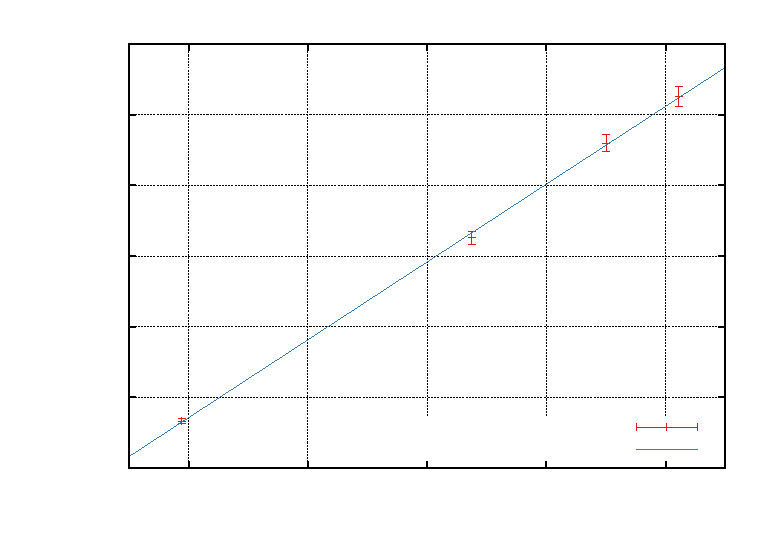
\includegraphics{./plots/rydberg_linearisierung}}%
    \gplfronttext
  \end{picture}%
\endgroup

	\caption{Linearisierung zur Bestimmung der Rydberg-Konstanten}
	\label{fig:rydberg_balmer}
\end{figure}
Die Anpassung ergibt für die Rydberg-Konstante:
\begin{align*}
	R_\mathrm{H} = \SI{11.016 +- 0.022}{\per\micro\metre} \text{,}
\end{align*}
bei einer Anpassungsgüte $\chi_\mathrm{red.}^2 = \num{0.263}$.
Literaturwerte:
\begin{align*}
	R_\infty = \SI{10.974}{\per\micro\metre}\\
	R_\mathrm{H} = \SI{10.969}{\per\micro\metre}\\
	R_\mathrm{D} = \SI{10.971}{\per\micro\metre}\\
\end{align*}

Zur Berechnung des Planckschen Wirkungsquantums aus der Rydberg-Konstanten $R_\mathrm{H}$ wird der Zusammenhang:
\begin{align*}
	R_\mathrm{H} = \left( 1 + \frac{m_e}{m_p} \right) R_\infty = \left( 1 + \frac{m_e}{m_p} \right) \frac{m_e e^4}{8 c \epsilon_0^2 h^3}
\end{align*}
genutzt, sodass für das Wirkungsquantum folgt:
\begin{align}
	\label{eq:wirkungsquantum_rydberg}
	h &= \sqrt[3]{\left( 1 + \frac{m_e}{m_p} \right) \frac{m_e e^4}{8 c \epsilon_0^2 R_\mathrm{H}}}
\end{align}
und mit Gaußsscher Fehlerfortpflanzung:
\begin{align*}
	\Delta h &= \frac{h \cdot \Delta R_\mathrm{H}}{3 R_\mathrm{H}} \text{,}
\end{align*}
wobei $h$ das berechnete Wirkungsquantum aus Gleichung \ref{eq:wirkungsquantum_rydberg} bezeichnet.
Mit den physikalischen Konstanten aus \cite{CODATA} und dem berechneten Wert für $R_\mathrm{H}$ folgt:
\begin{align*}
	h = \SI{6.619 +- 0.005e-34}{\joule\second}
\end{align*}

\subsubsection{Wellenlängen und Isotopieaufspaltung der Balmer-Linien bei Beobachtung mit der CCD-Kamera}

Es wird, wie bereits erwähnt, die jeweils beste Messung aus den vorliegenden Daten ausgewählt und grafisch dargestellt.
Dabei wurden mit \texttt{Gnuplot} (Least-Squares-Fit) zwei Gaußfunktionen an die Maxima mit folgender Fithypothese angepasst:
\begin{align}
f(x)&=\mathcal{G}_1(x)+\mathcal{G}_2(x) + d\qquad\text{mit}\\
\mathcal{G}_i(x)&=A\,\exp\left[-\frac{1}{2}\left(\frac{x-S_i}{\sigma_i}\right)^2\right]
\label{eq:fithypothese_gauss}
\end{align}
Diese sind zusammen mit den Messdaten in den Abbildungen \ref{fig:aufspaltung_rot} bis  \ref{fig:aufspaltung_violett} dargestellt.
Die Isotopieaufspaltung der violetten Balmer-Linie ist dabei so klein, dass sie in dem Versuch nicht gemessen werden konnte.
Der Vollständigkeit halber werden die Messwerte und eine daran angepasste Gaußkurve in dieses Protokoll aufgenommen, eine Auswertung ist damit jedoch nicht möglich gewesen.\\
\\
Für den Intensitätsfehler wurde mit Berücksichtigung der Mittelung der Messwerte über einen Zeitraum (die genommenen Daten unterliegen deswegen sehr kleinen Schwankungen) \SI{0.2}{\percent} für die Daten zur roten und türkisen Linie angenommen.
Im Fall der blauen Linie wurde aufgrund der geringen Intensität sehr lange im Programm VideoCom über die Messwerte gemittelt und deswegen \SI{0.1}{\percent} als Fehler für die Intensität gewählt.
Den Fehler des Winkels kann man zu \SI{0.0015}{\degree} abschätzen; dies folgt aus der Überlegung, dass ein Winkelbereich von ca. \SI{5.5}{\degree} auf \num{2048} Pixeln vermessen wurde.
\begin{figure}[h]
\centering
% GNUPLOT: LaTeX picture with Postscript
\begingroup
  \makeatletter
  \providecommand\color[2][]{%
    \GenericError{(gnuplot) \space\space\space\@spaces}{%
      Package color not loaded in conjunction with
      terminal option `colourtext'%
    }{See the gnuplot documentation for explanation.%
    }{Either use 'blacktext' in gnuplot or load the package
      color.sty in LaTeX.}%
    \renewcommand\color[2][]{}%
  }%
  \providecommand\includegraphics[2][]{%
    \GenericError{(gnuplot) \space\space\space\@spaces}{%
      Package graphicx or graphics not loaded%
    }{See the gnuplot documentation for explanation.%
    }{The gnuplot epslatex terminal needs graphicx.sty or graphics.sty.}%
    \renewcommand\includegraphics[2][]{}%
  }%
  \providecommand\rotatebox[2]{#2}%
  \@ifundefined{ifGPcolor}{%
    \newif\ifGPcolor
    \GPcolortrue
  }{}%
  \@ifundefined{ifGPblacktext}{%
    \newif\ifGPblacktext
    \GPblacktexttrue
  }{}%
  % define a \g@addto@macro without @ in the name:
  \let\gplgaddtomacro\g@addto@macro
  % define empty templates for all commands taking text:
  \gdef\gplbacktext{}%
  \gdef\gplfronttext{}%
  \makeatother
  \ifGPblacktext
    % no textcolor at all
    \def\colorrgb#1{}%
    \def\colorgray#1{}%
  \else
    % gray or color?
    \ifGPcolor
      \def\colorrgb#1{\color[rgb]{#1}}%
      \def\colorgray#1{\color[gray]{#1}}%
      \expandafter\def\csname LTw\endcsname{\color{white}}%
      \expandafter\def\csname LTb\endcsname{\color{black}}%
      \expandafter\def\csname LTa\endcsname{\color{black}}%
      \expandafter\def\csname LT0\endcsname{\color[rgb]{1,0,0}}%
      \expandafter\def\csname LT1\endcsname{\color[rgb]{0,1,0}}%
      \expandafter\def\csname LT2\endcsname{\color[rgb]{0,0,1}}%
      \expandafter\def\csname LT3\endcsname{\color[rgb]{1,0,1}}%
      \expandafter\def\csname LT4\endcsname{\color[rgb]{0,1,1}}%
      \expandafter\def\csname LT5\endcsname{\color[rgb]{1,1,0}}%
      \expandafter\def\csname LT6\endcsname{\color[rgb]{0,0,0}}%
      \expandafter\def\csname LT7\endcsname{\color[rgb]{1,0.3,0}}%
      \expandafter\def\csname LT8\endcsname{\color[rgb]{0.5,0.5,0.5}}%
    \else
      % gray
      \def\colorrgb#1{\color{black}}%
      \def\colorgray#1{\color[gray]{#1}}%
      \expandafter\def\csname LTw\endcsname{\color{white}}%
      \expandafter\def\csname LTb\endcsname{\color{black}}%
      \expandafter\def\csname LTa\endcsname{\color{black}}%
      \expandafter\def\csname LT0\endcsname{\color{black}}%
      \expandafter\def\csname LT1\endcsname{\color{black}}%
      \expandafter\def\csname LT2\endcsname{\color{black}}%
      \expandafter\def\csname LT3\endcsname{\color{black}}%
      \expandafter\def\csname LT4\endcsname{\color{black}}%
      \expandafter\def\csname LT5\endcsname{\color{black}}%
      \expandafter\def\csname LT6\endcsname{\color{black}}%
      \expandafter\def\csname LT7\endcsname{\color{black}}%
      \expandafter\def\csname LT8\endcsname{\color{black}}%
    \fi
  \fi
  \setlength{\unitlength}{0.0500bp}%
  \begin{picture}(7486.00,5040.00)%
    \gplgaddtomacro\gplbacktext{%
      \csname LTb\endcsname%
      \put(814,704){\makebox(0,0)[r]{\strut{} 0}}%
      \csname LTb\endcsname%
      \put(814,1286){\makebox(0,0)[r]{\strut{} 5}}%
      \csname LTb\endcsname%
      \put(814,1867){\makebox(0,0)[r]{\strut{} 10}}%
      \csname LTb\endcsname%
      \put(814,2449){\makebox(0,0)[r]{\strut{} 15}}%
      \csname LTb\endcsname%
      \put(814,3030){\makebox(0,0)[r]{\strut{} 20}}%
      \csname LTb\endcsname%
      \put(814,3612){\makebox(0,0)[r]{\strut{} 25}}%
      \csname LTb\endcsname%
      \put(814,4193){\makebox(0,0)[r]{\strut{} 30}}%
      \csname LTb\endcsname%
      \put(814,4775){\makebox(0,0)[r]{\strut{} 35}}%
      \csname LTb\endcsname%
      \put(946,484){\makebox(0,0){\strut{} 0.11}}%
      \csname LTb\endcsname%
      \put(1714,484){\makebox(0,0){\strut{} 0.12}}%
      \csname LTb\endcsname%
      \put(2482,484){\makebox(0,0){\strut{} 0.13}}%
      \csname LTb\endcsname%
      \put(3250,484){\makebox(0,0){\strut{} 0.14}}%
      \csname LTb\endcsname%
      \put(4018,484){\makebox(0,0){\strut{} 0.15}}%
      \csname LTb\endcsname%
      \put(4785,484){\makebox(0,0){\strut{} 0.16}}%
      \csname LTb\endcsname%
      \put(5553,484){\makebox(0,0){\strut{} 0.17}}%
      \csname LTb\endcsname%
      \put(6321,484){\makebox(0,0){\strut{} 0.18}}%
      \csname LTb\endcsname%
      \put(7089,484){\makebox(0,0){\strut{} 0.19}}%
      \put(176,2739){\rotatebox{-270}{\makebox(0,0){\strut{}Intensität $I$ / \si{\percent}}}}%
      \put(4017,154){\makebox(0,0){\strut{}Winkel $\alpha$ / \si{\degree}}}%
      \put(4017,4665){\makebox(0,0){\strut{}}}%
    }%
    \gplgaddtomacro\gplfronttext{%
      \csname LTb\endcsname%
      \put(6102,4602){\makebox(0,0)[r]{\strut{}Messwerte}}%
      \csname LTb\endcsname%
      \put(6102,4382){\makebox(0,0)[r]{\strut{}$\Sigma$}}%
      \csname LTb\endcsname%
      \put(6102,4162){\makebox(0,0)[r]{\strut{}$\mathcal{G}_1$}}%
      \csname LTb\endcsname%
      \put(6102,3942){\makebox(0,0)[r]{\strut{}$\mathcal{G}_2$}}%
      \csname LTb\endcsname%
      \put(6102,3722){\makebox(0,0)[r]{\strut{}$d$}}%
    }%
    \gplbacktext
    \put(0,0){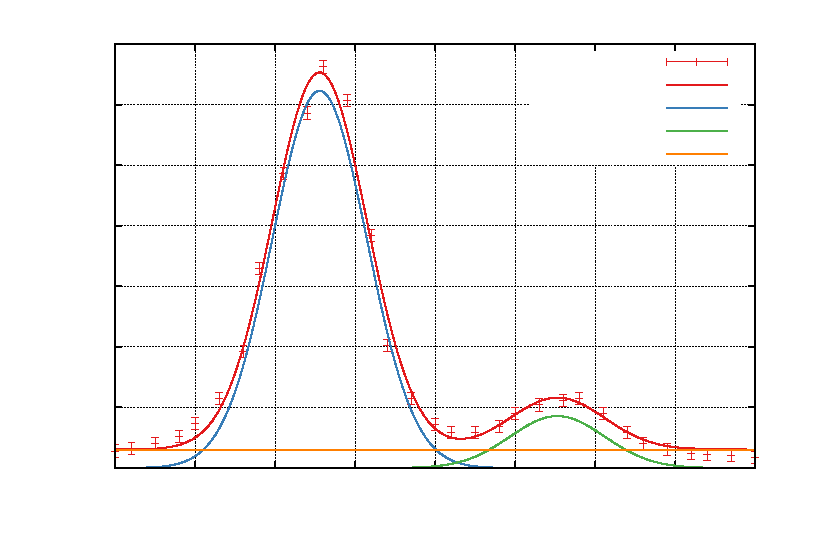
\includegraphics{./plots/aufspaltung/rot2}}%
    \gplfronttext
  \end{picture}%
\endgroup

\caption{Isotopieaufspaltung der roten Balmer-Linien von Wasserstoff und Deuterium}
\label{fig:aufspaltung_rot}
\end{figure}
\begin{figure}[h]
\centering
% GNUPLOT: LaTeX picture with Postscript
\begingroup
  \makeatletter
  \providecommand\color[2][]{%
    \GenericError{(gnuplot) \space\space\space\@spaces}{%
      Package color not loaded in conjunction with
      terminal option `colourtext'%
    }{See the gnuplot documentation for explanation.%
    }{Either use 'blacktext' in gnuplot or load the package
      color.sty in LaTeX.}%
    \renewcommand\color[2][]{}%
  }%
  \providecommand\includegraphics[2][]{%
    \GenericError{(gnuplot) \space\space\space\@spaces}{%
      Package graphicx or graphics not loaded%
    }{See the gnuplot documentation for explanation.%
    }{The gnuplot epslatex terminal needs graphicx.sty or graphics.sty.}%
    \renewcommand\includegraphics[2][]{}%
  }%
  \providecommand\rotatebox[2]{#2}%
  \@ifundefined{ifGPcolor}{%
    \newif\ifGPcolor
    \GPcolortrue
  }{}%
  \@ifundefined{ifGPblacktext}{%
    \newif\ifGPblacktext
    \GPblacktexttrue
  }{}%
  % define a \g@addto@macro without @ in the name:
  \let\gplgaddtomacro\g@addto@macro
  % define empty templates for all commands taking text:
  \gdef\gplbacktext{}%
  \gdef\gplfronttext{}%
  \makeatother
  \ifGPblacktext
    % no textcolor at all
    \def\colorrgb#1{}%
    \def\colorgray#1{}%
  \else
    % gray or color?
    \ifGPcolor
      \def\colorrgb#1{\color[rgb]{#1}}%
      \def\colorgray#1{\color[gray]{#1}}%
      \expandafter\def\csname LTw\endcsname{\color{white}}%
      \expandafter\def\csname LTb\endcsname{\color{black}}%
      \expandafter\def\csname LTa\endcsname{\color{black}}%
      \expandafter\def\csname LT0\endcsname{\color[rgb]{1,0,0}}%
      \expandafter\def\csname LT1\endcsname{\color[rgb]{0,1,0}}%
      \expandafter\def\csname LT2\endcsname{\color[rgb]{0,0,1}}%
      \expandafter\def\csname LT3\endcsname{\color[rgb]{1,0,1}}%
      \expandafter\def\csname LT4\endcsname{\color[rgb]{0,1,1}}%
      \expandafter\def\csname LT5\endcsname{\color[rgb]{1,1,0}}%
      \expandafter\def\csname LT6\endcsname{\color[rgb]{0,0,0}}%
      \expandafter\def\csname LT7\endcsname{\color[rgb]{1,0.3,0}}%
      \expandafter\def\csname LT8\endcsname{\color[rgb]{0.5,0.5,0.5}}%
    \else
      % gray
      \def\colorrgb#1{\color{black}}%
      \def\colorgray#1{\color[gray]{#1}}%
      \expandafter\def\csname LTw\endcsname{\color{white}}%
      \expandafter\def\csname LTb\endcsname{\color{black}}%
      \expandafter\def\csname LTa\endcsname{\color{black}}%
      \expandafter\def\csname LT0\endcsname{\color{black}}%
      \expandafter\def\csname LT1\endcsname{\color{black}}%
      \expandafter\def\csname LT2\endcsname{\color{black}}%
      \expandafter\def\csname LT3\endcsname{\color{black}}%
      \expandafter\def\csname LT4\endcsname{\color{black}}%
      \expandafter\def\csname LT5\endcsname{\color{black}}%
      \expandafter\def\csname LT6\endcsname{\color{black}}%
      \expandafter\def\csname LT7\endcsname{\color{black}}%
      \expandafter\def\csname LT8\endcsname{\color{black}}%
    \fi
  \fi
  \setlength{\unitlength}{0.0500bp}%
  \begin{picture}(7486.00,5040.00)%
    \gplgaddtomacro\gplbacktext{%
      \csname LTb\endcsname%
      \put(814,704){\makebox(0,0)[r]{\strut{} 0}}%
      \csname LTb\endcsname%
      \put(814,1383){\makebox(0,0)[r]{\strut{} 2}}%
      \csname LTb\endcsname%
      \put(814,2061){\makebox(0,0)[r]{\strut{} 4}}%
      \csname LTb\endcsname%
      \put(814,2740){\makebox(0,0)[r]{\strut{} 6}}%
      \csname LTb\endcsname%
      \put(814,3418){\makebox(0,0)[r]{\strut{} 8}}%
      \csname LTb\endcsname%
      \put(814,4097){\makebox(0,0)[r]{\strut{} 10}}%
      \csname LTb\endcsname%
      \put(814,4775){\makebox(0,0)[r]{\strut{} 12}}%
      \csname LTb\endcsname%
      \put(946,484){\makebox(0,0){\strut{} 0,06}}%
      \csname LTb\endcsname%
      \put(1629,484){\makebox(0,0){\strut{} 0,065}}%
      \csname LTb\endcsname%
      \put(2311,484){\makebox(0,0){\strut{} 0,07}}%
      \csname LTb\endcsname%
      \put(2994,484){\makebox(0,0){\strut{} 0,075}}%
      \csname LTb\endcsname%
      \put(3676,484){\makebox(0,0){\strut{} 0,08}}%
      \csname LTb\endcsname%
      \put(4359,484){\makebox(0,0){\strut{} 0,085}}%
      \csname LTb\endcsname%
      \put(5041,484){\makebox(0,0){\strut{} 0,09}}%
      \csname LTb\endcsname%
      \put(5724,484){\makebox(0,0){\strut{} 0,095}}%
      \csname LTb\endcsname%
      \put(6406,484){\makebox(0,0){\strut{} 0,1}}%
      \csname LTb\endcsname%
      \put(7089,484){\makebox(0,0){\strut{} 0,105}}%
      \put(176,2739){\rotatebox{-270}{\makebox(0,0){\strut{}Intensität $I$ / \si{\percent}}}}%
      \put(4017,154){\makebox(0,0){\strut{}Winkel $\alpha$ / \si{\degree}}}%
      \put(4017,4665){\makebox(0,0){\strut{}}}%
    }%
    \gplgaddtomacro\gplfronttext{%
      \csname LTb\endcsname%
      \put(6102,4602){\makebox(0,0)[r]{\strut{}Messwerte}}%
      \csname LTb\endcsname%
      \put(6102,4382){\makebox(0,0)[r]{\strut{}$\Sigma$}}%
      \csname LTb\endcsname%
      \put(6102,4162){\makebox(0,0)[r]{\strut{}$\mathcal{G}_1$}}%
      \csname LTb\endcsname%
      \put(6102,3942){\makebox(0,0)[r]{\strut{}$\mathcal{G}_2$}}%
      \csname LTb\endcsname%
      \put(6102,3722){\makebox(0,0)[r]{\strut{}$d$}}%
    }%
    \gplbacktext
    \put(0,0){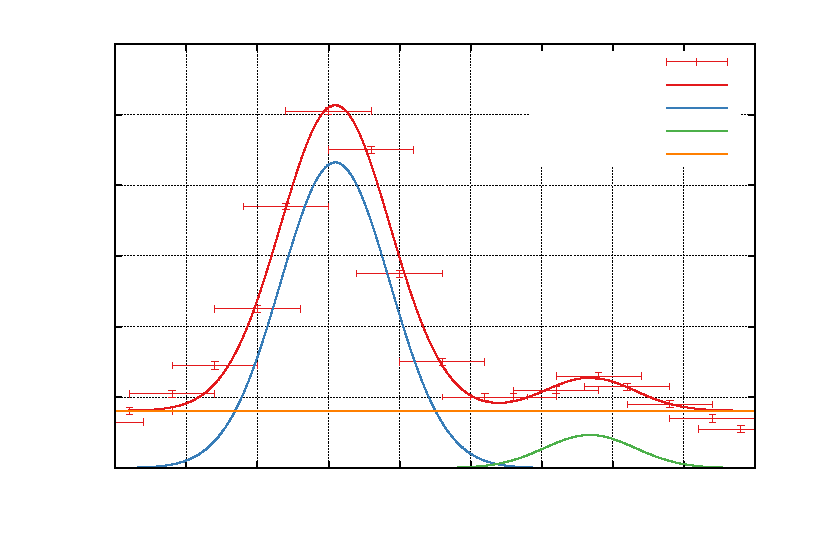
\includegraphics{./plots/aufspaltung/tuerkis1}}%
    \gplfronttext
  \end{picture}%
\endgroup

\caption{Isotopieaufspaltung der türkisen Balmer-Linien von Wasserstoff und Deuterium}
\label{fig:aufspaltung_tuerkis}
\end{figure}
\begin{figure}[h]
\centering
% GNUPLOT: LaTeX picture with Postscript
\begingroup
  \makeatletter
  \providecommand\color[2][]{%
    \GenericError{(gnuplot) \space\space\space\@spaces}{%
      Package color not loaded in conjunction with
      terminal option `colourtext'%
    }{See the gnuplot documentation for explanation.%
    }{Either use 'blacktext' in gnuplot or load the package
      color.sty in LaTeX.}%
    \renewcommand\color[2][]{}%
  }%
  \providecommand\includegraphics[2][]{%
    \GenericError{(gnuplot) \space\space\space\@spaces}{%
      Package graphicx or graphics not loaded%
    }{See the gnuplot documentation for explanation.%
    }{The gnuplot epslatex terminal needs graphicx.sty or graphics.sty.}%
    \renewcommand\includegraphics[2][]{}%
  }%
  \providecommand\rotatebox[2]{#2}%
  \@ifundefined{ifGPcolor}{%
    \newif\ifGPcolor
    \GPcolortrue
  }{}%
  \@ifundefined{ifGPblacktext}{%
    \newif\ifGPblacktext
    \GPblacktexttrue
  }{}%
  % define a \g@addto@macro without @ in the name:
  \let\gplgaddtomacro\g@addto@macro
  % define empty templates for all commands taking text:
  \gdef\gplbacktext{}%
  \gdef\gplfronttext{}%
  \makeatother
  \ifGPblacktext
    % no textcolor at all
    \def\colorrgb#1{}%
    \def\colorgray#1{}%
  \else
    % gray or color?
    \ifGPcolor
      \def\colorrgb#1{\color[rgb]{#1}}%
      \def\colorgray#1{\color[gray]{#1}}%
      \expandafter\def\csname LTw\endcsname{\color{white}}%
      \expandafter\def\csname LTb\endcsname{\color{black}}%
      \expandafter\def\csname LTa\endcsname{\color{black}}%
      \expandafter\def\csname LT0\endcsname{\color[rgb]{1,0,0}}%
      \expandafter\def\csname LT1\endcsname{\color[rgb]{0,1,0}}%
      \expandafter\def\csname LT2\endcsname{\color[rgb]{0,0,1}}%
      \expandafter\def\csname LT3\endcsname{\color[rgb]{1,0,1}}%
      \expandafter\def\csname LT4\endcsname{\color[rgb]{0,1,1}}%
      \expandafter\def\csname LT5\endcsname{\color[rgb]{1,1,0}}%
      \expandafter\def\csname LT6\endcsname{\color[rgb]{0,0,0}}%
      \expandafter\def\csname LT7\endcsname{\color[rgb]{1,0.3,0}}%
      \expandafter\def\csname LT8\endcsname{\color[rgb]{0.5,0.5,0.5}}%
    \else
      % gray
      \def\colorrgb#1{\color{black}}%
      \def\colorgray#1{\color[gray]{#1}}%
      \expandafter\def\csname LTw\endcsname{\color{white}}%
      \expandafter\def\csname LTb\endcsname{\color{black}}%
      \expandafter\def\csname LTa\endcsname{\color{black}}%
      \expandafter\def\csname LT0\endcsname{\color{black}}%
      \expandafter\def\csname LT1\endcsname{\color{black}}%
      \expandafter\def\csname LT2\endcsname{\color{black}}%
      \expandafter\def\csname LT3\endcsname{\color{black}}%
      \expandafter\def\csname LT4\endcsname{\color{black}}%
      \expandafter\def\csname LT5\endcsname{\color{black}}%
      \expandafter\def\csname LT6\endcsname{\color{black}}%
      \expandafter\def\csname LT7\endcsname{\color{black}}%
      \expandafter\def\csname LT8\endcsname{\color{black}}%
    \fi
  \fi
  \setlength{\unitlength}{0.0500bp}%
  \begin{picture}(7488.00,5040.00)%
    \gplgaddtomacro\gplbacktext{%
      \csname LTb\endcsname%
      \put(946,704){\makebox(0,0)[r]{\strut{} 0}}%
      \csname LTb\endcsname%
      \put(946,1286){\makebox(0,0)[r]{\strut{} 0,5}}%
      \csname LTb\endcsname%
      \put(946,1867){\makebox(0,0)[r]{\strut{} 1}}%
      \csname LTb\endcsname%
      \put(946,2449){\makebox(0,0)[r]{\strut{} 1,5}}%
      \csname LTb\endcsname%
      \put(946,3030){\makebox(0,0)[r]{\strut{} 2}}%
      \csname LTb\endcsname%
      \put(946,3612){\makebox(0,0)[r]{\strut{} 2,5}}%
      \csname LTb\endcsname%
      \put(946,4193){\makebox(0,0)[r]{\strut{} 3}}%
      \csname LTb\endcsname%
      \put(946,4775){\makebox(0,0)[r]{\strut{} 3,5}}%
      \csname LTb\endcsname%
      \put(1078,484){\makebox(0,0){\strut{}-0,03}}%
      \csname LTb\endcsname%
      \put(1746,484){\makebox(0,0){\strut{}-0,02}}%
      \csname LTb\endcsname%
      \put(2414,484){\makebox(0,0){\strut{}-0,01}}%
      \csname LTb\endcsname%
      \put(3082,484){\makebox(0,0){\strut{} 0}}%
      \csname LTb\endcsname%
      \put(3750,484){\makebox(0,0){\strut{} 0,01}}%
      \csname LTb\endcsname%
      \put(4419,484){\makebox(0,0){\strut{} 0,02}}%
      \csname LTb\endcsname%
      \put(5087,484){\makebox(0,0){\strut{} 0,03}}%
      \csname LTb\endcsname%
      \put(5755,484){\makebox(0,0){\strut{} 0,04}}%
      \csname LTb\endcsname%
      \put(6423,484){\makebox(0,0){\strut{} 0,05}}%
      \csname LTb\endcsname%
      \put(7091,484){\makebox(0,0){\strut{} 0,06}}%
      \put(176,2739){\rotatebox{-270}{\makebox(0,0){\strut{}Intensität $I$ / \si{\percent}}}}%
      \put(4084,154){\makebox(0,0){\strut{}Winkel $\delta$ / \si{\degree}}}%
      \put(4084,4665){\makebox(0,0){\strut{}}}%
    }%
    \gplgaddtomacro\gplfronttext{%
      \csname LTb\endcsname%
      \put(6104,4602){\makebox(0,0)[r]{\strut{}Messwerte}}%
      \csname LTb\endcsname%
      \put(6104,4382){\makebox(0,0)[r]{\strut{}$\Sigma$}}%
      \csname LTb\endcsname%
      \put(6104,4162){\makebox(0,0)[r]{\strut{}$\mathcal{G}_1$}}%
      \csname LTb\endcsname%
      \put(6104,3942){\makebox(0,0)[r]{\strut{}$\mathcal{G}_2$}}%
      \csname LTb\endcsname%
      \put(6104,3722){\makebox(0,0)[r]{\strut{}$d$}}%
    }%
    \gplbacktext
    \put(0,0){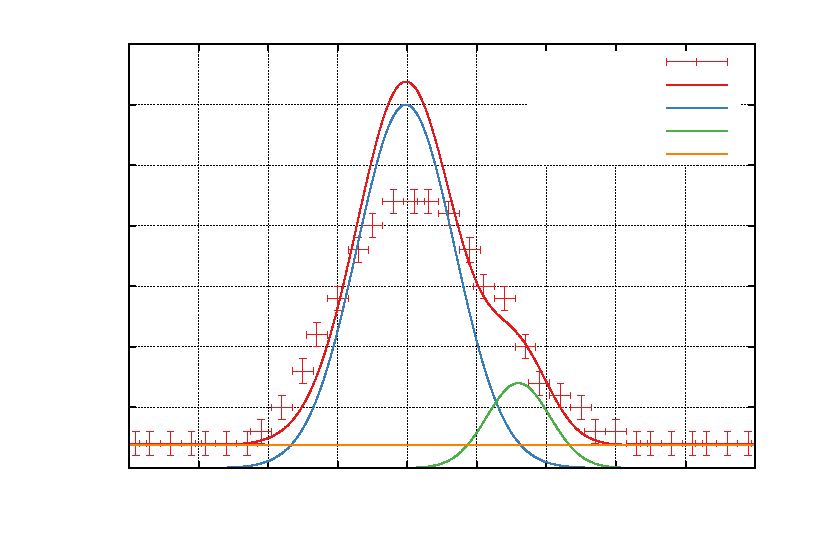
\includegraphics{./plots/aufspaltung/blau1}}%
    \gplfronttext
  \end{picture}%
\endgroup

\caption{Isotopieaufspaltung der blauen Balmer-Linien von Wasserstoff und Deuterium}
\label{fig:aufspaltung_blau}
\end{figure}
\begin{figure}[h]
\centering
% GNUPLOT: LaTeX picture with Postscript
\begingroup
  \makeatletter
  \providecommand\color[2][]{%
    \GenericError{(gnuplot) \space\space\space\@spaces}{%
      Package color not loaded in conjunction with
      terminal option `colourtext'%
    }{See the gnuplot documentation for explanation.%
    }{Either use 'blacktext' in gnuplot or load the package
      color.sty in LaTeX.}%
    \renewcommand\color[2][]{}%
  }%
  \providecommand\includegraphics[2][]{%
    \GenericError{(gnuplot) \space\space\space\@spaces}{%
      Package graphicx or graphics not loaded%
    }{See the gnuplot documentation for explanation.%
    }{The gnuplot epslatex terminal needs graphicx.sty or graphics.sty.}%
    \renewcommand\includegraphics[2][]{}%
  }%
  \providecommand\rotatebox[2]{#2}%
  \@ifundefined{ifGPcolor}{%
    \newif\ifGPcolor
    \GPcolortrue
  }{}%
  \@ifundefined{ifGPblacktext}{%
    \newif\ifGPblacktext
    \GPblacktexttrue
  }{}%
  % define a \g@addto@macro without @ in the name:
  \let\gplgaddtomacro\g@addto@macro
  % define empty templates for all commands taking text:
  \gdef\gplbacktext{}%
  \gdef\gplfronttext{}%
  \makeatother
  \ifGPblacktext
    % no textcolor at all
    \def\colorrgb#1{}%
    \def\colorgray#1{}%
  \else
    % gray or color?
    \ifGPcolor
      \def\colorrgb#1{\color[rgb]{#1}}%
      \def\colorgray#1{\color[gray]{#1}}%
      \expandafter\def\csname LTw\endcsname{\color{white}}%
      \expandafter\def\csname LTb\endcsname{\color{black}}%
      \expandafter\def\csname LTa\endcsname{\color{black}}%
      \expandafter\def\csname LT0\endcsname{\color[rgb]{1,0,0}}%
      \expandafter\def\csname LT1\endcsname{\color[rgb]{0,1,0}}%
      \expandafter\def\csname LT2\endcsname{\color[rgb]{0,0,1}}%
      \expandafter\def\csname LT3\endcsname{\color[rgb]{1,0,1}}%
      \expandafter\def\csname LT4\endcsname{\color[rgb]{0,1,1}}%
      \expandafter\def\csname LT5\endcsname{\color[rgb]{1,1,0}}%
      \expandafter\def\csname LT6\endcsname{\color[rgb]{0,0,0}}%
      \expandafter\def\csname LT7\endcsname{\color[rgb]{1,0.3,0}}%
      \expandafter\def\csname LT8\endcsname{\color[rgb]{0.5,0.5,0.5}}%
    \else
      % gray
      \def\colorrgb#1{\color{black}}%
      \def\colorgray#1{\color[gray]{#1}}%
      \expandafter\def\csname LTw\endcsname{\color{white}}%
      \expandafter\def\csname LTb\endcsname{\color{black}}%
      \expandafter\def\csname LTa\endcsname{\color{black}}%
      \expandafter\def\csname LT0\endcsname{\color{black}}%
      \expandafter\def\csname LT1\endcsname{\color{black}}%
      \expandafter\def\csname LT2\endcsname{\color{black}}%
      \expandafter\def\csname LT3\endcsname{\color{black}}%
      \expandafter\def\csname LT4\endcsname{\color{black}}%
      \expandafter\def\csname LT5\endcsname{\color{black}}%
      \expandafter\def\csname LT6\endcsname{\color{black}}%
      \expandafter\def\csname LT7\endcsname{\color{black}}%
      \expandafter\def\csname LT8\endcsname{\color{black}}%
    \fi
  \fi
  \setlength{\unitlength}{0.0500bp}%
  \begin{picture}(7488.00,5040.00)%
    \gplgaddtomacro\gplbacktext{%
      \csname LTb\endcsname%
      \put(946,704){\makebox(0,0)[r]{\strut{} 0}}%
      \csname LTb\endcsname%
      \put(946,1518){\makebox(0,0)[r]{\strut{} 0,1}}%
      \csname LTb\endcsname%
      \put(946,2332){\makebox(0,0)[r]{\strut{} 0,2}}%
      \csname LTb\endcsname%
      \put(946,3147){\makebox(0,0)[r]{\strut{} 0,3}}%
      \csname LTb\endcsname%
      \put(946,3961){\makebox(0,0)[r]{\strut{} 0,4}}%
      \csname LTb\endcsname%
      \put(946,4775){\makebox(0,0)[r]{\strut{} 0,5}}%
      \csname LTb\endcsname%
      \put(1078,484){\makebox(0,0){\strut{} 0,015}}%
      \csname LTb\endcsname%
      \put(1830,484){\makebox(0,0){\strut{} 0,02}}%
      \csname LTb\endcsname%
      \put(2581,484){\makebox(0,0){\strut{} 0,025}}%
      \csname LTb\endcsname%
      \put(3333,484){\makebox(0,0){\strut{} 0,03}}%
      \csname LTb\endcsname%
      \put(4085,484){\makebox(0,0){\strut{} 0,035}}%
      \csname LTb\endcsname%
      \put(4836,484){\makebox(0,0){\strut{} 0,04}}%
      \csname LTb\endcsname%
      \put(5588,484){\makebox(0,0){\strut{} 0,045}}%
      \csname LTb\endcsname%
      \put(6339,484){\makebox(0,0){\strut{} 0,05}}%
      \csname LTb\endcsname%
      \put(7091,484){\makebox(0,0){\strut{} 0,055}}%
      \put(176,2739){\rotatebox{-270}{\makebox(0,0){\strut{}Intensität $I$ / \si{\percent}}}}%
      \put(4084,154){\makebox(0,0){\strut{}Winkel $\delta$ / \si{\degree}}}%
      \put(4084,4665){\makebox(0,0){\strut{}}}%
    }%
    \gplgaddtomacro\gplfronttext{%
      \csname LTb\endcsname%
      \put(6104,4602){\makebox(0,0)[r]{\strut{}Messwerte}}%
      \csname LTb\endcsname%
      \put(6104,4382){\makebox(0,0)[r]{\strut{}$\mathcal{G}$}}%
      \csname LTb\endcsname%
      \put(6104,4162){\makebox(0,0)[r]{\strut{}$d$}}%
    }%
    \gplbacktext
    \put(0,0){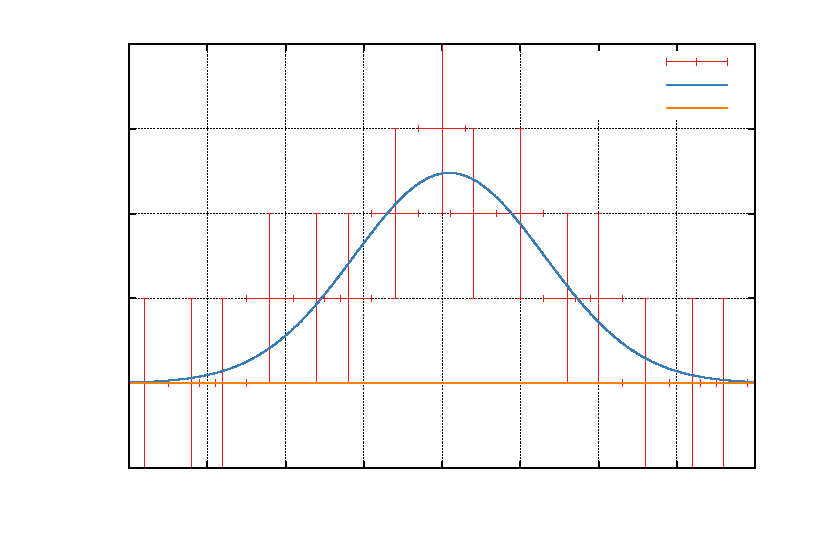
\includegraphics{./plots/aufspaltung/violett2}}%
    \gplfronttext
  \end{picture}%
\endgroup

\caption{nicht sichtbare Isotopieaufspaltung der violetten Balmer-Linien von Wasserstoff und Deuterium}
\label{fig:aufspaltung_violett}
\end{figure}
\FloatBarrier
In Abbildung \ref{fig:aufspaltung_blau} ist offensichtlich, dass die Amplitude der Maxima nicht korrekt angepasst wurde.
Da die Linien sehr schmal und die Aufspaltung sehr gering ist, liegen hier wenige Messdaten vor, an die die Funktion angepasst werden kann.
Dabei ist die Anpassung auch noch sehr stark von der Wahl der Anfangsbedingungen abhängig.
Einzig die für diese Anpassung gewählten Anfangsbedingungen (der Anfangswert der Amplitude des Hauptmaximas wurde bei der Anpassung übernommen) liefert ein halbwegs sinnvolles Ergebnis.
Da die Amplitude zur Auswertung nicht benötigt wird und die Schwerpunkte der Gaußkurven sinnvoll erscheinen, ist dies die unserer Meinung nach beste Möglichkeit, auswertbare Daten zu erhalten und diese werden zur Anpassung in der Auswertung nutzen.

In Tabelle \ref{tab:balmer_ccd_messwerte} sind die Messwerte, die der Auswertung zugrunde liegen, dargestellt.
Die Ergebnisse der Anpassungen für die Schwerpunkte $S_1$ (Wasserstofflinie) und $S_2$ (Deuteriumlinie) durch \texttt{Gnuplot} sind dort ebenfalls eingetragen worden.
Aus der Differenz der Schwerpunkte errechnen wir in \ref{tab:balmer_ccd_auswertung} die Winkelaufspaltung $\Delta\beta$ zwischen der Wasserstoff- und Deuteriumlinie.\\
\\
Wie in Abschnitt \ref{sssec:balmer_okular_aufspaltung} nutzen wir Formel \eqref{eq:gitter_differenzial}:
\begin{align*}
\Delta\lambda=g\,\cos(\beta)\Delta\beta
\end{align*}
Damit kann die Wellenlängenaufspaltung $\Delta\lambda$ der beiden Linien aus der Winkelaufspaltung und dem Reflexionswinkel ausgerechnet werden.
Den Reflexionswinkel $\beta$ erhält man gemäß Abbildung \ref{fig:winkelverhaeltnis} und Formel  \eqref{eq:reflexionswinkel} aus den in Tabelle \ref{tab:balmer_ccd_messwerte} eingetragenen Gitterwinkeln bei festem Bankwinkel $\omega_\text{B}$= \SI{150}{\degree}.
Die so gefundenen Werte sind ebenso wie die Fehler bereits in der Tabelle \ref{tab:balmer_ccd_auswertung} eingetragen.
\begin{table}[h]
\centering
\resizebox{\columnwidth}{!}{%
\begin{tabular}{lllll}
	\toprule
	Farbe & Gitterwinkel $\omega_\text{G}$ / \si{\degree} & Wellenlänge $\lambda$ / \si{\nano\metre} & Schwerpunkt 1 / \si{\degree} & Schwerpunkt 2 / \si{\degree} \\
	\midrule
	Rot		& \num{70.5+-0.5} 	& \num{652.8+-4.1} & \num{0.13556+-0.00025} &	\num{0.16529+-0.00204}\\
	Türkis	& \num{53+-0.5}		& \num{487.6+-5.2} & \num{0.07548+-0.00024} &	\num{0.09338+-0.00220}\\
	Blau 	& \num{48+-0.5}		& \num{431.4+-5.4} & \num{0.00980+-0.00090} &	\num{0.02598+-0.00281}\\
	Violett & \num{46+-0.5}		& \num{407.9+-5.5} & n.v. & n.v. \\
	\bottomrule
\end{tabular}}
\caption{Messwerte bei der Beobachtung der Balmer-Linien mit der CCD-Kamera}
\label{tab:balmer_ccd_messwerte}
\end{table}

\begin{table}[h]
\centering
\begin{tabular}{lllll}
	\toprule
	Farbe & Schwerpunkt 1 / \si{\degree} & Schwerpunkt 2 / \si{\degree} & Winkelaufspaltung $\Delta\beta$ / \si{\degree} & Aufspaltung $\Delta\lambda$ \si{\nano\metre}  \\
	\midrule
	Rot & \num{0.13556+-0.00015} &	\num{0.16529+-0.00104} &	\num{0.000519+-0.000018} &	\num{0.1618+-0.0058} \\
	Türkis & \num{0.07548+-0.00014} &	\num{0.09338+-0.00120} &	\num{0.000312+-0.000021} &	\num{0.1179+-0.0080} \\
	Blau & \num{0.00980+-0.00090} &	\num{0.02598+-0.00281} &	\num{0.000282+-0.000051} &	\num{0.1101+-0.0200} \\
	\bottomrule
\end{tabular}
\caption{Auswertung der Balmer-Linien mit der CCD-Kamera}
\label{tab:balmer_ccd_auswertung}
\end{table}
\noindent
Zum Vergleich errechnen wir mit \eqref{eq:rydberg_formel} die folgenden theoretischen Werte:
\begin{align}
\Delta\lambda_\alpha=\SI{179}{\pico\metre}\\
\Delta\lambda_\beta=\SI{132}{\pico\metre}\\
\Delta\lambda_\gamma=\SI{118}{\pico\metre}
\end{align}
Die von uns gemessenen Werte der roten und türkisen Linie liegen unter den theoretischen Werten für die Wellenlängenverschiebung, der für die blaue darüber.
Der Literaturwert der roten Balmer-Linie liegt nicht mehr im $1$-$\sigma$-Bereich der gemessenen Isotopieaufspaltung, die anderen beiden Aufspaltungen sind unter Berücksichtigung der Fehlergrenzen mit dem Literaturwert verträglich.
Die Aufspaltung der blauen Linie ist unter Berücksichtigung der schlechten Anpassung, die der Auswertung zugrunde liegt, gut bestimmt worden.
\FloatBarrier
\subsection{Weitergehende Überlegungen}

\subsubsection{Erklärung weiterer Linien im Spektrum der Balmer-Lampe}

Bei der Messung der Balmer-Linien sind auch andere Linien, die offensichtlich nicht zum Balmer-Spektrum gehören, zu sehen. Bei etwa \SI{590}{\nano\metre} konnte eine gelbe Linie beobachtet werden, die den beiden Natrium-D-Linien bei \SI{590.0}{\nano\metre} bzw \SI{590.6}{\nano\metre} zugeordnet werden kann.
Ursache für die Beobachtung ist ein kleiner Anteil Natrium in der Balmer-Lampe, der bei der Gasentladung entstehendes Wasser binden soll.

\subsubsection{Dopplerverbreiterung der Linien}
Zur Abschätzung der Dopplerverbreiterung wird, unter der Annahme, dass die Temperatur der Balmer-Lampe \SI{1000}{\kelvin} beträgt, Formel \eqref{eq:doppler} verwendet.
Die damit gefundenen Werte sind für die von uns beobachteten Wellenlängen in Tabelle \ref{tab:doppler} in der letzten Spalte eingetragen worden.
\begin{table}[h]
\centering
\resizebox{\columnwidth}{!}{%
\begin{tabular}{lllll}
\toprule
Wellenlänge /\si{\nano\metre} & $\sigma_1$ / \si{\degree} & $\mathrm{HWB}_\mathrm{CCD}$ / \si{\milli\radian} & $\mathrm{HWB}_\mathrm{CCD}$ / \si{\pico\metre} & $\mathrm{HWB}_\mathrm{Doppler}$ / \si{\pico\metre} \\
\midrule
\num{652.8}& \num{0.005912}       & \num{0.243} & \num{75.8}  & \num{14.78} \\
\num{487.6}& \num{0.003847}       & \num{0.158} & \num{59.7}  & \num{11.00} \\
\num{431.4}& \num{0.010917}       & \num{0.449} & \num{174.9} & \num{9.77}  \\
\num{407.9}& \num{0.006064}       & \num{0.249} & \num{98.2}  & \num{9.24}  \\
\bottomrule
\end{tabular}
}
\caption{Werte zur Dopplerverbreiterung}
\label{tab:doppler}
\end{table}
In den anderen Spalten wurde die Linienbreite aus den mit der CCD-Kamera gemessenen Daten berechnet.
Dazu wurden die Schwankungsbreiten $\sigma_1$ des Hauptmaximums (Wasserstofflinie) aus den Anpassungen in Abbildungen \ref{fig:aufspaltung_rot}, \ref{fig:aufspaltung_tuerkis} und \ref{fig:aufspaltung_violett} in die Tabelle eingetragen.
Die Anpassung für die blaue Linie (wie in \ref{fig:aufspaltung_blau}) wurde in \ref{fig:doppler_blau} mit einer neuen Fithypothese mit nur einer Gaußfunktion und Untergrund wiederholt, um einen sinnvolleren Wert für die Schwankungsbreite zu erhalten.
\begin{figure}[h]
\centering
% GNUPLOT: LaTeX picture with Postscript
\begingroup
  \makeatletter
  \providecommand\color[2][]{%
    \GenericError{(gnuplot) \space\space\space\@spaces}{%
      Package color not loaded in conjunction with
      terminal option `colourtext'%
    }{See the gnuplot documentation for explanation.%
    }{Either use 'blacktext' in gnuplot or load the package
      color.sty in LaTeX.}%
    \renewcommand\color[2][]{}%
  }%
  \providecommand\includegraphics[2][]{%
    \GenericError{(gnuplot) \space\space\space\@spaces}{%
      Package graphicx or graphics not loaded%
    }{See the gnuplot documentation for explanation.%
    }{The gnuplot epslatex terminal needs graphicx.sty or graphics.sty.}%
    \renewcommand\includegraphics[2][]{}%
  }%
  \providecommand\rotatebox[2]{#2}%
  \@ifundefined{ifGPcolor}{%
    \newif\ifGPcolor
    \GPcolortrue
  }{}%
  \@ifundefined{ifGPblacktext}{%
    \newif\ifGPblacktext
    \GPblacktexttrue
  }{}%
  % define a \g@addto@macro without @ in the name:
  \let\gplgaddtomacro\g@addto@macro
  % define empty templates for all commands taking text:
  \gdef\gplbacktext{}%
  \gdef\gplfronttext{}%
  \makeatother
  \ifGPblacktext
    % no textcolor at all
    \def\colorrgb#1{}%
    \def\colorgray#1{}%
  \else
    % gray or color?
    \ifGPcolor
      \def\colorrgb#1{\color[rgb]{#1}}%
      \def\colorgray#1{\color[gray]{#1}}%
      \expandafter\def\csname LTw\endcsname{\color{white}}%
      \expandafter\def\csname LTb\endcsname{\color{black}}%
      \expandafter\def\csname LTa\endcsname{\color{black}}%
      \expandafter\def\csname LT0\endcsname{\color[rgb]{1,0,0}}%
      \expandafter\def\csname LT1\endcsname{\color[rgb]{0,1,0}}%
      \expandafter\def\csname LT2\endcsname{\color[rgb]{0,0,1}}%
      \expandafter\def\csname LT3\endcsname{\color[rgb]{1,0,1}}%
      \expandafter\def\csname LT4\endcsname{\color[rgb]{0,1,1}}%
      \expandafter\def\csname LT5\endcsname{\color[rgb]{1,1,0}}%
      \expandafter\def\csname LT6\endcsname{\color[rgb]{0,0,0}}%
      \expandafter\def\csname LT7\endcsname{\color[rgb]{1,0.3,0}}%
      \expandafter\def\csname LT8\endcsname{\color[rgb]{0.5,0.5,0.5}}%
    \else
      % gray
      \def\colorrgb#1{\color{black}}%
      \def\colorgray#1{\color[gray]{#1}}%
      \expandafter\def\csname LTw\endcsname{\color{white}}%
      \expandafter\def\csname LTb\endcsname{\color{black}}%
      \expandafter\def\csname LTa\endcsname{\color{black}}%
      \expandafter\def\csname LT0\endcsname{\color{black}}%
      \expandafter\def\csname LT1\endcsname{\color{black}}%
      \expandafter\def\csname LT2\endcsname{\color{black}}%
      \expandafter\def\csname LT3\endcsname{\color{black}}%
      \expandafter\def\csname LT4\endcsname{\color{black}}%
      \expandafter\def\csname LT5\endcsname{\color{black}}%
      \expandafter\def\csname LT6\endcsname{\color{black}}%
      \expandafter\def\csname LT7\endcsname{\color{black}}%
      \expandafter\def\csname LT8\endcsname{\color{black}}%
    \fi
  \fi
  \setlength{\unitlength}{0.0500bp}%
  \begin{picture}(7488.00,5040.00)%
    \gplgaddtomacro\gplbacktext{%
      \csname LTb\endcsname%
      \put(946,704){\makebox(0,0)[r]{\strut{} 0}}%
      \csname LTb\endcsname%
      \put(946,1518){\makebox(0,0)[r]{\strut{} 0,5}}%
      \csname LTb\endcsname%
      \put(946,2332){\makebox(0,0)[r]{\strut{} 1}}%
      \csname LTb\endcsname%
      \put(946,3147){\makebox(0,0)[r]{\strut{} 1,5}}%
      \csname LTb\endcsname%
      \put(946,3961){\makebox(0,0)[r]{\strut{} 2}}%
      \csname LTb\endcsname%
      \put(946,4775){\makebox(0,0)[r]{\strut{} 2,5}}%
      \csname LTb\endcsname%
      \put(1078,484){\makebox(0,0){\strut{}-0,03}}%
      \csname LTb\endcsname%
      \put(1746,484){\makebox(0,0){\strut{}-0,02}}%
      \csname LTb\endcsname%
      \put(2414,484){\makebox(0,0){\strut{}-0,01}}%
      \csname LTb\endcsname%
      \put(3082,484){\makebox(0,0){\strut{} 0}}%
      \csname LTb\endcsname%
      \put(3750,484){\makebox(0,0){\strut{} 0,01}}%
      \csname LTb\endcsname%
      \put(4419,484){\makebox(0,0){\strut{} 0,02}}%
      \csname LTb\endcsname%
      \put(5087,484){\makebox(0,0){\strut{} 0,03}}%
      \csname LTb\endcsname%
      \put(5755,484){\makebox(0,0){\strut{} 0,04}}%
      \csname LTb\endcsname%
      \put(6423,484){\makebox(0,0){\strut{} 0,05}}%
      \csname LTb\endcsname%
      \put(7091,484){\makebox(0,0){\strut{} 0,06}}%
      \put(176,2739){\rotatebox{-270}{\makebox(0,0){\strut{}Intensität $I$ / \si{\percent}}}}%
      \put(4084,154){\makebox(0,0){\strut{}Winkel $\delta$ / \si{\degree}}}%
      \put(4084,4665){\makebox(0,0){\strut{}}}%
    }%
    \gplgaddtomacro\gplfronttext{%
      \csname LTb\endcsname%
      \put(6104,4602){\makebox(0,0)[r]{\strut{}Messwerte}}%
      \csname LTb\endcsname%
      \put(6104,4382){\makebox(0,0)[r]{\strut{}$\Sigma$}}%
      \csname LTb\endcsname%
      \put(6104,4162){\makebox(0,0)[r]{\strut{}$\mathcal{G}_1$}}%
      \csname LTb\endcsname%
      \put(6104,3942){\makebox(0,0)[r]{\strut{}$d$}}%
    }%
    \gplbacktext
    \put(0,0){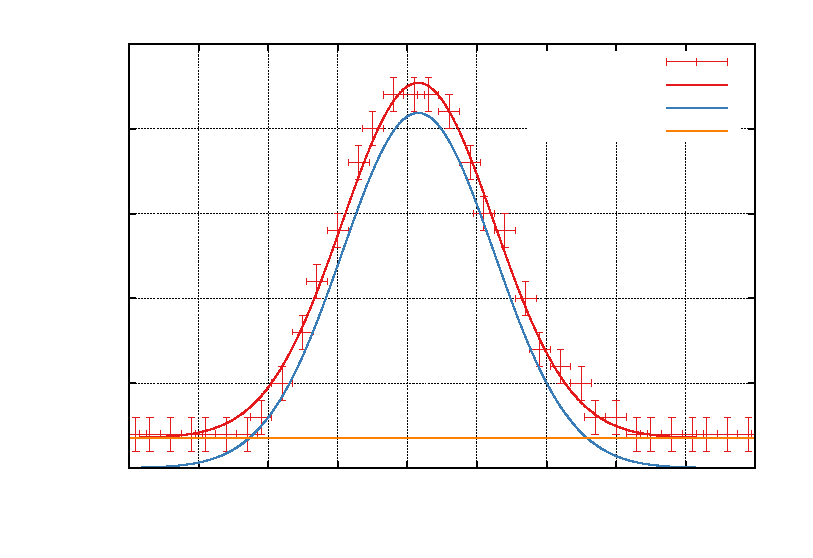
\includegraphics{./plots/doppler_blau1}}%
    \gplfronttext
  \end{picture}%
\endgroup

\caption{Anpassung von einer Gaußkurve an die Messwerte der blauen Balmer-Linie}
\label{fig:doppler_blau}
\end{figure}
Die gefundenen Schwankungsbreiten wurden mit dem Faktor $2\sqrt{2\ln2}$ multipliziert, um die Halbwertsbreite der angepassten Gaußfunktion zu erhalten.
Mit \eqref{eq:gitter_differenzial} wurde dieser Wert anschließend in die Wellenlänge umgerechnet, um die gemessenen Werte mit den theoretischen zu vergleichen.
Die gemessenen Linienbreiten für die rote und türkise Linie liefern dabei plausible Werte, die der anderen beiden Linien erscheinen deutlich zu groß.
Ursache hierfür sind vor allem die Anpassungen mit nur einer Gauß-Kurve, wobei eine sinnvolle Anpassung mit zwei Gauß-Kurven aufgrund weniger Messwerte nicht möglich war.
Darum soll im Weiteren nur noch auf die Breiten der roten und türkisen Linien eingegangen werden.

Die gefundenen Linienbreiten sind um den Faktor \num{5} größer als der erwartete Wert, wobei die natürliche Linienbreite mit $\frac{\delta\nu}{\nu}\approx \num{e-8}$ deutlich schmäler ist als die hier auftretenden Werte, so dass diese für die hier getroffene Abschätzung vernachlässigt werden kann.
Da die Druckverbreiterung proportional zu Druck bzw. Wirkungsquerschnitt ist (vgl. \cite{gerthsen}), scheidet sie aufgrund der in diesem Versuch in der Lampe herrschenden Bedingungen (kein besonders hoher Druck, kleiner Wirkungsquerschnitt) als Ursache für die Linienverbreiterung aus.
Es handelt sich deswegen anscheinend um Fehler in der Anpassung oder Berechnung, die auf die gefundenen (zu großen) Halbwertsbreiten führen.

\subsubsection{Auflösungsvermögen des Gitters}
Das Auflösungsvermögen eines Gitters ist durch
\begin{align*}
\mathcal{R}=\frac{\lambda}{\Delta\lambda}=n\,N
\end{align*}
gegeben, mit der Anzahl beleuchteter Spalte $N$ und der beobachteten Ordnung $n$. Unter der Annahme, dass das Gitter über die volle Breite (\SI{25}{\milli\metre}) beleuchtet ist und die Linien jeweils in der ersten Beugungsordnung beobachtet werden, erhält man mit der Gitterkonstante $g=\SI{409.9}{\nano\metre}$ als obere Grenze für das Auflösungsvermögen:
\begin{align*}
\mathcal{R} = \frac{\SI{25}{\milli\metre}}{\SI{409.9}{\nano\metre}} \approx 61000
\end{align*}

\subsection{Fazit}
Insgesamt ist der Versuchsteil als gelungen zu bewerten.
Trotz leichter Schwierigkeiten, Messwerte für die blaue und violette Linie aufzunehmen konnte die Aufspaltung der messbaren Linien gut durchgeführt und berechnet werden.
Die mit dem Okular gefundenen Werte stimmen innerhalb der Fehlergrenzen mit den Literaturwerten überein, wobei durch die Beobachtung mit dem Auge der Fehler zwischen recht großen \SI{11}{\percent} und \SI{25}{\percent} liegt.
Im Vergleich zu den theoretischen Werten für die Isotopieaufspaltung liegen die mit der CCD-Kamera gefundenen Werte in der gleichen Größenordnung, allerdings teilweise außerhalb des $1$-$\sigma$-Bereichs um den Mittelwert.
Ursache hierfür ist offenbar die Anpassung durch \textit{Gnuplot} und die Tatsache, dass die Linien nicht ganz zentral in der CCD-Zeile lagen.
Die Abschätzung der Dopplerverbreiterung hingegen liefert keine sinnvollen Werte und übersteigt die erwarteten Werte etwa um den Faktor $5$.
Eine eindeutige Ursache konnte hierfür nicht gefunden werden.
WIRKUNGSQUANTUM FAZIT

% BIBLIOGRAPHIE

% Maximale Anzahl der Einträge in Klammer
% Zitieren mit \cite{lamport94}
\begin{thebibliography}{9}
\bibitem{prak_uheidelberg}
	Dr. J. Wagner.
	\emph{Physikalisches Anfängerpraktikum der Universität Heidelberg} (Versuch 35).
	\url{http://www.physi.uni-heidelberg.de/Einrichtungen/AP/anleitungen/35_Fotoeffekt_01.pdf} (Letzter Abruf: 09. Dezember 2014).

\bibitem{demtroder}
	Wolfgang Demtröder,
	\emph{Experimentalphysik 3: Atome, Moleküle und Festkörper}.
	Springer Verlag,
	4. Auflage

\bibitem{NISTSpectra}
	Kramida, A., Ralchenko, Yu., Reader, J., and NIST ASD Team (2014).
	\emph{NIST Atomic Spectra Database} (ver. 5.2).
	\url{http://physics.nist.gov/asd} (Letzter Abruf: 07. Dezember 2014).
	National Institute of Standards and Technology, Gaithersburg, MD.

\bibitem{CODATA}
	P.J. Mohr, B.N. Taylor, and D.B. Newell (2011),
	\emph{The 2010 CODATA Recommended Values of the Fundamental Physical Constants}.
	\url{http://physics.nist.gov/constants} (Letzer Abruf: 08. Dezember 2014).
	National Institute of Standards and Technology, Gaithersburg, MD.
	
\bibitem{gerthsen}
	Dieter Meschede,
	\emph{Gerthsen Physik}.
	Springer Verlag,
	23. Auflage

\bibitem{crc}
	David R. Lide (ed),
	\emph{CRC Handbook of Chemistry and Physics},
	84th Edition. CRC Press. Boca Raton, Florida, 2003;
	Section 12: Properties of Solids --
	\emph{Electron Work Function of the Elements}
 
\end{thebibliography}

% APPENDIX
\begin{appendix}
\section{Anhang}
\subsection{Kennlinien des Photostroms}
\label{app:kennlinien}
\FloatBarrier
% Messung 365nm
\begin{figure}
	\centering
	% GNUPLOT: LaTeX picture with Postscript
\begingroup
  \makeatletter
  \providecommand\color[2][]{%
    \GenericError{(gnuplot) \space\space\space\@spaces}{%
      Package color not loaded in conjunction with
      terminal option `colourtext'%
    }{See the gnuplot documentation for explanation.%
    }{Either use 'blacktext' in gnuplot or load the package
      color.sty in LaTeX.}%
    \renewcommand\color[2][]{}%
  }%
  \providecommand\includegraphics[2][]{%
    \GenericError{(gnuplot) \space\space\space\@spaces}{%
      Package graphicx or graphics not loaded%
    }{See the gnuplot documentation for explanation.%
    }{The gnuplot epslatex terminal needs graphicx.sty or graphics.sty.}%
    \renewcommand\includegraphics[2][]{}%
  }%
  \providecommand\rotatebox[2]{#2}%
  \@ifundefined{ifGPcolor}{%
    \newif\ifGPcolor
    \GPcolortrue
  }{}%
  \@ifundefined{ifGPblacktext}{%
    \newif\ifGPblacktext
    \GPblacktexttrue
  }{}%
  % define a \g@addto@macro without @ in the name:
  \let\gplgaddtomacro\g@addto@macro
  % define empty templates for all commands taking text:
  \gdef\gplbacktext{}%
  \gdef\gplfronttext{}%
  \makeatother
  \ifGPblacktext
    % no textcolor at all
    \def\colorrgb#1{}%
    \def\colorgray#1{}%
  \else
    % gray or color?
    \ifGPcolor
      \def\colorrgb#1{\color[rgb]{#1}}%
      \def\colorgray#1{\color[gray]{#1}}%
      \expandafter\def\csname LTw\endcsname{\color{white}}%
      \expandafter\def\csname LTb\endcsname{\color{black}}%
      \expandafter\def\csname LTa\endcsname{\color{black}}%
      \expandafter\def\csname LT0\endcsname{\color[rgb]{1,0,0}}%
      \expandafter\def\csname LT1\endcsname{\color[rgb]{0,1,0}}%
      \expandafter\def\csname LT2\endcsname{\color[rgb]{0,0,1}}%
      \expandafter\def\csname LT3\endcsname{\color[rgb]{1,0,1}}%
      \expandafter\def\csname LT4\endcsname{\color[rgb]{0,1,1}}%
      \expandafter\def\csname LT5\endcsname{\color[rgb]{1,1,0}}%
      \expandafter\def\csname LT6\endcsname{\color[rgb]{0,0,0}}%
      \expandafter\def\csname LT7\endcsname{\color[rgb]{1,0.3,0}}%
      \expandafter\def\csname LT8\endcsname{\color[rgb]{0.5,0.5,0.5}}%
    \else
      % gray
      \def\colorrgb#1{\color{black}}%
      \def\colorgray#1{\color[gray]{#1}}%
      \expandafter\def\csname LTw\endcsname{\color{white}}%
      \expandafter\def\csname LTb\endcsname{\color{black}}%
      \expandafter\def\csname LTa\endcsname{\color{black}}%
      \expandafter\def\csname LT0\endcsname{\color{black}}%
      \expandafter\def\csname LT1\endcsname{\color{black}}%
      \expandafter\def\csname LT2\endcsname{\color{black}}%
      \expandafter\def\csname LT3\endcsname{\color{black}}%
      \expandafter\def\csname LT4\endcsname{\color{black}}%
      \expandafter\def\csname LT5\endcsname{\color{black}}%
      \expandafter\def\csname LT6\endcsname{\color{black}}%
      \expandafter\def\csname LT7\endcsname{\color{black}}%
      \expandafter\def\csname LT8\endcsname{\color{black}}%
    \fi
  \fi
  \setlength{\unitlength}{0.0500bp}%
  \begin{picture}(6480.00,4320.00)%
    \gplgaddtomacro\gplbacktext{%
      \csname LTb\endcsname%
      \put(946,704){\makebox(0,0)[r]{\strut{} 0}}%
      \csname LTb\endcsname%
      \put(946,1076){\makebox(0,0)[r]{\strut{} 0,5}}%
      \csname LTb\endcsname%
      \put(946,1449){\makebox(0,0)[r]{\strut{} 1}}%
      \csname LTb\endcsname%
      \put(946,1821){\makebox(0,0)[r]{\strut{} 1,5}}%
      \csname LTb\endcsname%
      \put(946,2193){\makebox(0,0)[r]{\strut{} 2}}%
      \csname LTb\endcsname%
      \put(946,2566){\makebox(0,0)[r]{\strut{} 2,5}}%
      \csname LTb\endcsname%
      \put(946,2938){\makebox(0,0)[r]{\strut{} 3}}%
      \csname LTb\endcsname%
      \put(946,3310){\makebox(0,0)[r]{\strut{} 3,5}}%
      \csname LTb\endcsname%
      \put(946,3683){\makebox(0,0)[r]{\strut{} 4}}%
      \csname LTb\endcsname%
      \put(946,4055){\makebox(0,0)[r]{\strut{} 4,5}}%
      \csname LTb\endcsname%
      \put(1078,484){\makebox(0,0){\strut{} 0}}%
      \csname LTb\endcsname%
      \put(2079,484){\makebox(0,0){\strut{} 0,5}}%
      \csname LTb\endcsname%
      \put(3080,484){\makebox(0,0){\strut{} 1}}%
      \csname LTb\endcsname%
      \put(4081,484){\makebox(0,0){\strut{} 1,5}}%
      \csname LTb\endcsname%
      \put(5082,484){\makebox(0,0){\strut{} 2}}%
      \csname LTb\endcsname%
      \put(6083,484){\makebox(0,0){\strut{} 2,5}}%
      \put(176,2379){\rotatebox{-270}{\makebox(0,0){\strut{}$\sqrt{I-I_0} \, / \, \si{\nano\ampere^{1/2}}$}}}%
      \put(3580,154){\makebox(0,0){\strut{}$U \, / \, \si{\volt}$}}%
      \put(3580,3945){\makebox(0,0){\strut{}}}%
    }%
    \gplgaddtomacro\gplfronttext{%
      \csname LTb\endcsname%
      \put(5096,3882){\makebox(0,0)[r]{\strut{}Messung 1}}%
      \csname LTb\endcsname%
      \put(5096,3662){\makebox(0,0)[r]{\strut{}Regressionsgerade 1}}%
      \csname LTb\endcsname%
      \put(5096,3442){\makebox(0,0)[r]{\strut{}Messung 2}}%
      \csname LTb\endcsname%
      \put(5096,3222){\makebox(0,0)[r]{\strut{}Regressionsgerade 2}}%
    }%
    \gplbacktext
    \put(0,0){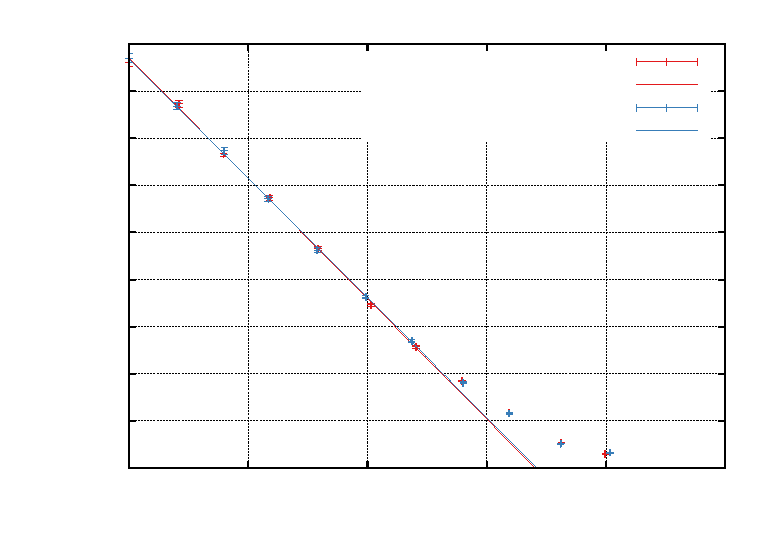
\includegraphics{./plots/photo/kennlinien_365nm}}%
    \gplfronttext
  \end{picture}%
\endgroup

	\caption{Linearisierte Kennlinie zur Grenzspannungsbestimmung $\lambda = \SI{365}{\nano\metre}$}
	\label{fig:kennlinien_365nm}
\end{figure}

\begin{table}
	\centering
	\begin{subtable}{0.5\textwidth}
		\centering
		\vspace{0pt}
		\resizebox{0.95\columnwidth}{!}{%
			\begin{tabular}{SSS}
	\toprule
	{$U$ / \si{\volt}} & {$I-I_0$ / \si{\nano\ampere}} & {$\Delta (I-I_0)$ / \si{\nano\ampere}} \\
	\midrule
0.001 & 18.522 & 0.373 \\
0.209 & 14.922 & 0.301 \\
0.397 & 11.122 & 0.225 \\
0.590 & 8.222  & 0.167 \\
0.793 & 5.422  & 0.111 \\
1.015 & 3.002  & 0.062 \\
1.203 & 1.652  & 0.035 \\
1.395 & 0.852  & 0.019 \\
1.595 & 0.342  & 0.009 \\
1.813 & 0.072  & 0.004 \\
1.997 & 0.022  & 0.003 \\
	\bottomrule
\end{tabular}

		}
		\caption{Messung 1}
	\end{subtable}%
	\begin{subtable}{0.5\textwidth}
		\centering
		\vspace{0pt}
		\resizebox{0.95\columnwidth}{!}{%
			\begin{tabular}{SSS}
	\toprule
	{$U$ / \si{\volt}} & {$I-I_0$ / \si{\nano\ampere}} & {$\Delta (I-I_0)$ / \si{\nano\ampere}} \\
	\midrule
0.001 & 18.927 & 0.381 \\
0.201 & 14.727 & 0.297 \\
0.400 & 11.327 & 0.229 \\
0.583 & 8.167  & 0.165 \\
0.790 & 5.347  & 0.109 \\
0.992 & 3.287  & 0.068 \\
1.185 & 1.817  & 0.038 \\
1.402 & 0.817  & 0.018 \\
1.595 & 0.337  & 0.009 \\
1.810 & 0.067  & 0.003 \\
2.016 & 0.027  & 0.003 \\
	\bottomrule
\end{tabular}

		}
		\caption{Messung 2}
	\end{subtable}

	\caption{Kennlinien der Photozelle f\"ur Licht der Wellenl\"ange $\lambda=\SI{365}{\nano\metre}$}
\end{table}



% Messung 405nm
\begin{figure}
	\centering
	% GNUPLOT: LaTeX picture with Postscript
\begingroup
  \makeatletter
  \providecommand\color[2][]{%
    \GenericError{(gnuplot) \space\space\space\@spaces}{%
      Package color not loaded in conjunction with
      terminal option `colourtext'%
    }{See the gnuplot documentation for explanation.%
    }{Either use 'blacktext' in gnuplot or load the package
      color.sty in LaTeX.}%
    \renewcommand\color[2][]{}%
  }%
  \providecommand\includegraphics[2][]{%
    \GenericError{(gnuplot) \space\space\space\@spaces}{%
      Package graphicx or graphics not loaded%
    }{See the gnuplot documentation for explanation.%
    }{The gnuplot epslatex terminal needs graphicx.sty or graphics.sty.}%
    \renewcommand\includegraphics[2][]{}%
  }%
  \providecommand\rotatebox[2]{#2}%
  \@ifundefined{ifGPcolor}{%
    \newif\ifGPcolor
    \GPcolortrue
  }{}%
  \@ifundefined{ifGPblacktext}{%
    \newif\ifGPblacktext
    \GPblacktexttrue
  }{}%
  % define a \g@addto@macro without @ in the name:
  \let\gplgaddtomacro\g@addto@macro
  % define empty templates for all commands taking text:
  \gdef\gplbacktext{}%
  \gdef\gplfronttext{}%
  \makeatother
  \ifGPblacktext
    % no textcolor at all
    \def\colorrgb#1{}%
    \def\colorgray#1{}%
  \else
    % gray or color?
    \ifGPcolor
      \def\colorrgb#1{\color[rgb]{#1}}%
      \def\colorgray#1{\color[gray]{#1}}%
      \expandafter\def\csname LTw\endcsname{\color{white}}%
      \expandafter\def\csname LTb\endcsname{\color{black}}%
      \expandafter\def\csname LTa\endcsname{\color{black}}%
      \expandafter\def\csname LT0\endcsname{\color[rgb]{1,0,0}}%
      \expandafter\def\csname LT1\endcsname{\color[rgb]{0,1,0}}%
      \expandafter\def\csname LT2\endcsname{\color[rgb]{0,0,1}}%
      \expandafter\def\csname LT3\endcsname{\color[rgb]{1,0,1}}%
      \expandafter\def\csname LT4\endcsname{\color[rgb]{0,1,1}}%
      \expandafter\def\csname LT5\endcsname{\color[rgb]{1,1,0}}%
      \expandafter\def\csname LT6\endcsname{\color[rgb]{0,0,0}}%
      \expandafter\def\csname LT7\endcsname{\color[rgb]{1,0.3,0}}%
      \expandafter\def\csname LT8\endcsname{\color[rgb]{0.5,0.5,0.5}}%
    \else
      % gray
      \def\colorrgb#1{\color{black}}%
      \def\colorgray#1{\color[gray]{#1}}%
      \expandafter\def\csname LTw\endcsname{\color{white}}%
      \expandafter\def\csname LTb\endcsname{\color{black}}%
      \expandafter\def\csname LTa\endcsname{\color{black}}%
      \expandafter\def\csname LT0\endcsname{\color{black}}%
      \expandafter\def\csname LT1\endcsname{\color{black}}%
      \expandafter\def\csname LT2\endcsname{\color{black}}%
      \expandafter\def\csname LT3\endcsname{\color{black}}%
      \expandafter\def\csname LT4\endcsname{\color{black}}%
      \expandafter\def\csname LT5\endcsname{\color{black}}%
      \expandafter\def\csname LT6\endcsname{\color{black}}%
      \expandafter\def\csname LT7\endcsname{\color{black}}%
      \expandafter\def\csname LT8\endcsname{\color{black}}%
    \fi
  \fi
  \setlength{\unitlength}{0.0500bp}%
  \begin{picture}(7200.00,5040.00)%
    \gplgaddtomacro\gplbacktext{%
      \csname LTb\endcsname%
      \put(946,704){\makebox(0,0)[r]{\strut{} 0}}%
      \csname LTb\endcsname%
      \put(946,1383){\makebox(0,0)[r]{\strut{} 0.5}}%
      \csname LTb\endcsname%
      \put(946,2061){\makebox(0,0)[r]{\strut{} 1}}%
      \csname LTb\endcsname%
      \put(946,2740){\makebox(0,0)[r]{\strut{} 1.5}}%
      \csname LTb\endcsname%
      \put(946,3418){\makebox(0,0)[r]{\strut{} 2}}%
      \csname LTb\endcsname%
      \put(946,4097){\makebox(0,0)[r]{\strut{} 2.5}}%
      \csname LTb\endcsname%
      \put(946,4775){\makebox(0,0)[r]{\strut{} 3}}%
      \csname LTb\endcsname%
      \put(1078,484){\makebox(0,0){\strut{} 0}}%
      \csname LTb\endcsname%
      \put(1714,484){\makebox(0,0){\strut{} 0.2}}%
      \csname LTb\endcsname%
      \put(2350,484){\makebox(0,0){\strut{} 0.4}}%
      \csname LTb\endcsname%
      \put(2986,484){\makebox(0,0){\strut{} 0.6}}%
      \csname LTb\endcsname%
      \put(3622,484){\makebox(0,0){\strut{} 0.8}}%
      \csname LTb\endcsname%
      \put(4259,484){\makebox(0,0){\strut{} 1}}%
      \csname LTb\endcsname%
      \put(4895,484){\makebox(0,0){\strut{} 1.2}}%
      \csname LTb\endcsname%
      \put(5531,484){\makebox(0,0){\strut{} 1.4}}%
      \csname LTb\endcsname%
      \put(6167,484){\makebox(0,0){\strut{} 1.6}}%
      \csname LTb\endcsname%
      \put(6803,484){\makebox(0,0){\strut{} 1.8}}%
      \put(176,2739){\rotatebox{-270}{\makebox(0,0){\strut{}$\sqrt{I-I_0} \, / \, \si{\nano\ampere^{1/2}}$}}}%
      \put(3940,154){\makebox(0,0){\strut{}$U \, / \, \si{\volt}$}}%
      \put(3940,4665){\makebox(0,0){\strut{}}}%
    }%
    \gplgaddtomacro\gplfronttext{%
      \csname LTb\endcsname%
      \put(5816,4602){\makebox(0,0)[r]{\strut{}Messung 1}}%
      \csname LTb\endcsname%
      \put(5816,4382){\makebox(0,0)[r]{\strut{}Regressionsgerade 1}}%
      \csname LTb\endcsname%
      \put(5816,4162){\makebox(0,0)[r]{\strut{}Messung 2}}%
      \csname LTb\endcsname%
      \put(5816,3942){\makebox(0,0)[r]{\strut{}Regressionsgerade 2}}%
    }%
    \gplbacktext
    \put(0,0){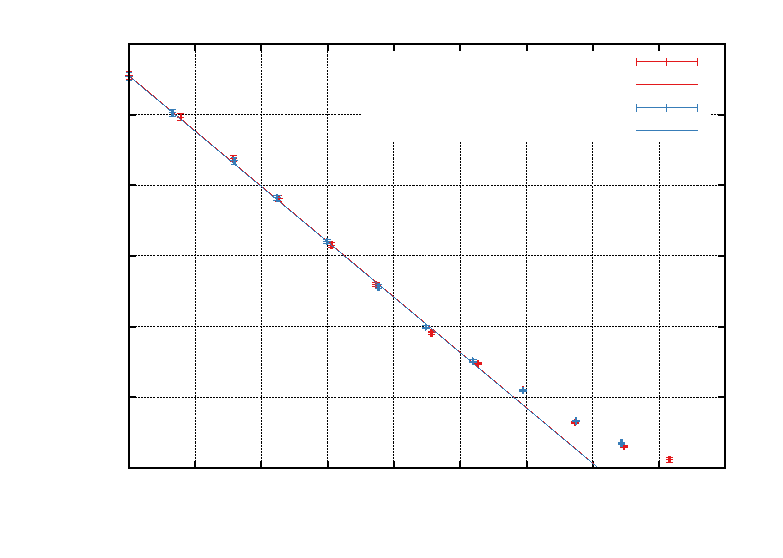
\includegraphics{./plots/photo/kennlinien_405nm}}%
    \gplfronttext
  \end{picture}%
\endgroup

	\caption{Linearisierte Kennlinie zur Grenzspannungsbestimmung $\lambda = \SI{405}{\nano\metre}$}
	\label{fig:kennlinien_405nm}
\end{figure}

\begin{table}
	\centering
	\begin{subtable}{0.5\textwidth}
		\centering
		\vspace{0pt}
		\resizebox{0.95\columnwidth}{!}{%
			\begin{tabular}{SSS}
	\toprule
	{$U$ / \si{\volt}} & {$I-I_0$ / \si{\nano\ampere}} & {$\Delta (I-I_0)$ / \si{\nano\ampere}} \\
	\midrule
0.001 & 7.714 & 0.157 \\
0.156 & 6.164 & 0.126 \\
0.315 & 4.784 & 0.098 \\
0.452 & 3.634 & 0.075 \\
0.611 & 2.484 & 0.052 \\
0.745 & 1.684 & 0.036 \\
0.913 & 0.914 & 0.021 \\
1.053 & 0.544 & 0.013 \\
1.189 & 0.304 & 0.008 \\
1.346 & 0.104 & 0.004 \\
1.494 & 0.024 & 0.003 \\
1.632 & 0.004 & 0.003 \\
	\bottomrule
\end{tabular}

		}
		\caption{Messung 1}
	\end{subtable}%
	\begin{subtable}{0.5\textwidth}
		\centering
		\vspace{0pt}
		\resizebox{0.95\columnwidth}{!}{%
			\begin{tabular}{SSS}
	\toprule
	{$U$ / \si{\volt}} & {$I-I_0$ / \si{\nano\ampere}} & {$\Delta (I-I_0)$ / \si{\nano\ampere}} \\
	\midrule
0.001 & 7.661 & 0.155 \\
0.132 & 6.321 & 0.129 \\
0.318 & 4.721 & 0.097 \\
0.447 & 3.651 & 0.075 \\
0.598 & 2.571 & 0.054 \\
0.753 & 1.641 & 0.035 \\
0.896 & 0.991 & 0.022 \\
1.038 & 0.571 & 0.014 \\
1.189 & 0.301 & 0.008 \\
1.349 & 0.111 & 0.004 \\
1.487 & 0.031 & 0.003 \\
	\bottomrule
\end{tabular}


		}
		\caption{Messung 2}
	\end{subtable}

	\caption{Kennlinien der Photozelle f\"ur Licht der Wellenl\"ange $\lambda = \SI{405}{\nano\metre}$}
\end{table}



% Messung 436nm
\begin{figure}
	\centering
	% GNUPLOT: LaTeX picture with Postscript
\begingroup
  \makeatletter
  \providecommand\color[2][]{%
    \GenericError{(gnuplot) \space\space\space\@spaces}{%
      Package color not loaded in conjunction with
      terminal option `colourtext'%
    }{See the gnuplot documentation for explanation.%
    }{Either use 'blacktext' in gnuplot or load the package
      color.sty in LaTeX.}%
    \renewcommand\color[2][]{}%
  }%
  \providecommand\includegraphics[2][]{%
    \GenericError{(gnuplot) \space\space\space\@spaces}{%
      Package graphicx or graphics not loaded%
    }{See the gnuplot documentation for explanation.%
    }{The gnuplot epslatex terminal needs graphicx.sty or graphics.sty.}%
    \renewcommand\includegraphics[2][]{}%
  }%
  \providecommand\rotatebox[2]{#2}%
  \@ifundefined{ifGPcolor}{%
    \newif\ifGPcolor
    \GPcolortrue
  }{}%
  \@ifundefined{ifGPblacktext}{%
    \newif\ifGPblacktext
    \GPblacktexttrue
  }{}%
  % define a \g@addto@macro without @ in the name:
  \let\gplgaddtomacro\g@addto@macro
  % define empty templates for all commands taking text:
  \gdef\gplbacktext{}%
  \gdef\gplfronttext{}%
  \makeatother
  \ifGPblacktext
    % no textcolor at all
    \def\colorrgb#1{}%
    \def\colorgray#1{}%
  \else
    % gray or color?
    \ifGPcolor
      \def\colorrgb#1{\color[rgb]{#1}}%
      \def\colorgray#1{\color[gray]{#1}}%
      \expandafter\def\csname LTw\endcsname{\color{white}}%
      \expandafter\def\csname LTb\endcsname{\color{black}}%
      \expandafter\def\csname LTa\endcsname{\color{black}}%
      \expandafter\def\csname LT0\endcsname{\color[rgb]{1,0,0}}%
      \expandafter\def\csname LT1\endcsname{\color[rgb]{0,1,0}}%
      \expandafter\def\csname LT2\endcsname{\color[rgb]{0,0,1}}%
      \expandafter\def\csname LT3\endcsname{\color[rgb]{1,0,1}}%
      \expandafter\def\csname LT4\endcsname{\color[rgb]{0,1,1}}%
      \expandafter\def\csname LT5\endcsname{\color[rgb]{1,1,0}}%
      \expandafter\def\csname LT6\endcsname{\color[rgb]{0,0,0}}%
      \expandafter\def\csname LT7\endcsname{\color[rgb]{1,0.3,0}}%
      \expandafter\def\csname LT8\endcsname{\color[rgb]{0.5,0.5,0.5}}%
    \else
      % gray
      \def\colorrgb#1{\color{black}}%
      \def\colorgray#1{\color[gray]{#1}}%
      \expandafter\def\csname LTw\endcsname{\color{white}}%
      \expandafter\def\csname LTb\endcsname{\color{black}}%
      \expandafter\def\csname LTa\endcsname{\color{black}}%
      \expandafter\def\csname LT0\endcsname{\color{black}}%
      \expandafter\def\csname LT1\endcsname{\color{black}}%
      \expandafter\def\csname LT2\endcsname{\color{black}}%
      \expandafter\def\csname LT3\endcsname{\color{black}}%
      \expandafter\def\csname LT4\endcsname{\color{black}}%
      \expandafter\def\csname LT5\endcsname{\color{black}}%
      \expandafter\def\csname LT6\endcsname{\color{black}}%
      \expandafter\def\csname LT7\endcsname{\color{black}}%
      \expandafter\def\csname LT8\endcsname{\color{black}}%
    \fi
  \fi
  \setlength{\unitlength}{0.0500bp}%
  \begin{picture}(7200.00,5040.00)%
    \gplgaddtomacro\gplbacktext{%
      \csname LTb\endcsname%
      \put(946,704){\makebox(0,0)[r]{\strut{} 0}}%
      \csname LTb\endcsname%
      \put(946,1213){\makebox(0,0)[r]{\strut{} 0.5}}%
      \csname LTb\endcsname%
      \put(946,1722){\makebox(0,0)[r]{\strut{} 1}}%
      \csname LTb\endcsname%
      \put(946,2231){\makebox(0,0)[r]{\strut{} 1.5}}%
      \csname LTb\endcsname%
      \put(946,2740){\makebox(0,0)[r]{\strut{} 2}}%
      \csname LTb\endcsname%
      \put(946,3248){\makebox(0,0)[r]{\strut{} 2.5}}%
      \csname LTb\endcsname%
      \put(946,3757){\makebox(0,0)[r]{\strut{} 3}}%
      \csname LTb\endcsname%
      \put(946,4266){\makebox(0,0)[r]{\strut{} 3.5}}%
      \csname LTb\endcsname%
      \put(946,4775){\makebox(0,0)[r]{\strut{} 4}}%
      \csname LTb\endcsname%
      \put(1078,484){\makebox(0,0){\strut{} 0}}%
      \csname LTb\endcsname%
      \put(1794,484){\makebox(0,0){\strut{} 0.2}}%
      \csname LTb\endcsname%
      \put(2509,484){\makebox(0,0){\strut{} 0.4}}%
      \csname LTb\endcsname%
      \put(3225,484){\makebox(0,0){\strut{} 0.6}}%
      \csname LTb\endcsname%
      \put(3941,484){\makebox(0,0){\strut{} 0.8}}%
      \csname LTb\endcsname%
      \put(4656,484){\makebox(0,0){\strut{} 1}}%
      \csname LTb\endcsname%
      \put(5372,484){\makebox(0,0){\strut{} 1.2}}%
      \csname LTb\endcsname%
      \put(6087,484){\makebox(0,0){\strut{} 1.4}}%
      \csname LTb\endcsname%
      \put(6803,484){\makebox(0,0){\strut{} 1.6}}%
      \put(176,2739){\rotatebox{-270}{\makebox(0,0){\strut{}$\sqrt{I-I_0} \, / \, \si{\nano\ampere^{1/2}}$}}}%
      \put(3940,154){\makebox(0,0){\strut{}$U \, / \, \si{\volt}$}}%
      \put(3940,4665){\makebox(0,0){\strut{}}}%
    }%
    \gplgaddtomacro\gplfronttext{%
      \csname LTb\endcsname%
      \put(5816,4602){\makebox(0,0)[r]{\strut{}Messung 1}}%
      \csname LTb\endcsname%
      \put(5816,4382){\makebox(0,0)[r]{\strut{}Regressionsgerade 1}}%
      \csname LTb\endcsname%
      \put(5816,4162){\makebox(0,0)[r]{\strut{}Messung 2}}%
      \csname LTb\endcsname%
      \put(5816,3942){\makebox(0,0)[r]{\strut{}Regressionsgerade 2}}%
    }%
    \gplbacktext
    \put(0,0){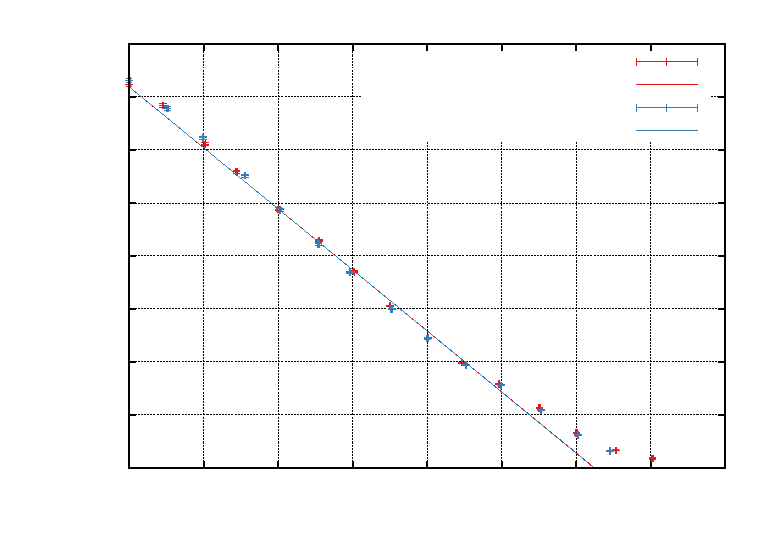
\includegraphics{./plots/photo/kennlinien_436nm}}%
    \gplfronttext
  \end{picture}%
\endgroup

	\caption{Linearisierte Kennlinie zur Grenzspannungsbestimmung $\lambda = \SI{436}{\nano\metre}$}
	\label{fig:kennlinien_436nm}
\end{figure}

\begin{table}
	\centering
	\begin{subtable}{0.5\textwidth}
		\centering
		\vspace{0pt}
		\resizebox{0.95\columnwidth}{!}{%
			\begin{tabular}{SSS}
	\toprule
	{$U$ / \si{\volt}} & {$I-I_0$ / \si{\nano\ampere}} & {$\Delta (I-I_0)$ / \si{\nano\ampere}} \\
	\midrule
0.001 & 13.120 & 0.265 \\
0.091 & 11.708 & 0.237 \\
0.204 & 9.328  & 0.189 \\
0.289 & 7.808  & 0.159 \\
0.401 & 5.958  & 0.122 \\
0.510 & 4.608  & 0.095 \\
0.604 & 3.428  & 0.071 \\
0.700 & 2.338  & 0.049 \\
0.802 & 1.498  & 0.032 \\
0.894 & 0.988  & 0.022 \\
0.993 & 0.628  & 0.015 \\
1.102 & 0.318  & 0.009 \\
1.201 & 0.108  & 0.005 \\
1.306 & 0.028  & 0.003 \\
1.405 & 0.008  & 0.003 \\
	\bottomrule
\end{tabular}

		}
		\caption{Messung 1}
	\end{subtable}%
	\begin{subtable}{0.5\textwidth}
		\centering
		\vspace{0pt}
		\resizebox{0.95\columnwidth}{!}{%
			\begin{tabular}{SSS}
	\toprule
	{$U$ / \si{\volt}} & {$I-I_0$ / \si{\nano\ampere}} & {$\Delta (I-I_0)$ / \si{\nano\ampere}} \\
	\midrule
0.001 & 13.372 & 0.270 \\
0.103 & 11.522 & 0.233 \\
0.199 & 9.712  & 0.196 \\
0.311 & 7.622  & 0.155 \\
0.405 & 5.942  & 0.121 \\
0.508 & 4.482  & 0.092 \\
0.593 & 3.432  & 0.071 \\
0.705 & 2.262  & 0.047 \\
0.801 & 1.512  & 0.032 \\
0.904 & 0.962  & 0.021 \\
0.998 & 0.622  & 0.015 \\
1.106 & 0.312  & 0.008 \\
1.205 & 0.112  & 0.004 \\
1.291 & 0.042  & 0.003 \\
	\bottomrule
\end{tabular}

		}
		\caption{Messung 2}
	\end{subtable}

	\caption{Kennlinien der Photozelle f\"ur Licht der Wellenl\"ange $\lambda = \SI{436}{\nano\metre}$}
\end{table}



% Messung 546nm
\begin{figure}
	\centering
	% GNUPLOT: LaTeX picture with Postscript
\begingroup
  \makeatletter
  \providecommand\color[2][]{%
    \GenericError{(gnuplot) \space\space\space\@spaces}{%
      Package color not loaded in conjunction with
      terminal option `colourtext'%
    }{See the gnuplot documentation for explanation.%
    }{Either use 'blacktext' in gnuplot or load the package
      color.sty in LaTeX.}%
    \renewcommand\color[2][]{}%
  }%
  \providecommand\includegraphics[2][]{%
    \GenericError{(gnuplot) \space\space\space\@spaces}{%
      Package graphicx or graphics not loaded%
    }{See the gnuplot documentation for explanation.%
    }{The gnuplot epslatex terminal needs graphicx.sty or graphics.sty.}%
    \renewcommand\includegraphics[2][]{}%
  }%
  \providecommand\rotatebox[2]{#2}%
  \@ifundefined{ifGPcolor}{%
    \newif\ifGPcolor
    \GPcolortrue
  }{}%
  \@ifundefined{ifGPblacktext}{%
    \newif\ifGPblacktext
    \GPblacktexttrue
  }{}%
  % define a \g@addto@macro without @ in the name:
  \let\gplgaddtomacro\g@addto@macro
  % define empty templates for all commands taking text:
  \gdef\gplbacktext{}%
  \gdef\gplfronttext{}%
  \makeatother
  \ifGPblacktext
    % no textcolor at all
    \def\colorrgb#1{}%
    \def\colorgray#1{}%
  \else
    % gray or color?
    \ifGPcolor
      \def\colorrgb#1{\color[rgb]{#1}}%
      \def\colorgray#1{\color[gray]{#1}}%
      \expandafter\def\csname LTw\endcsname{\color{white}}%
      \expandafter\def\csname LTb\endcsname{\color{black}}%
      \expandafter\def\csname LTa\endcsname{\color{black}}%
      \expandafter\def\csname LT0\endcsname{\color[rgb]{1,0,0}}%
      \expandafter\def\csname LT1\endcsname{\color[rgb]{0,1,0}}%
      \expandafter\def\csname LT2\endcsname{\color[rgb]{0,0,1}}%
      \expandafter\def\csname LT3\endcsname{\color[rgb]{1,0,1}}%
      \expandafter\def\csname LT4\endcsname{\color[rgb]{0,1,1}}%
      \expandafter\def\csname LT5\endcsname{\color[rgb]{1,1,0}}%
      \expandafter\def\csname LT6\endcsname{\color[rgb]{0,0,0}}%
      \expandafter\def\csname LT7\endcsname{\color[rgb]{1,0.3,0}}%
      \expandafter\def\csname LT8\endcsname{\color[rgb]{0.5,0.5,0.5}}%
    \else
      % gray
      \def\colorrgb#1{\color{black}}%
      \def\colorgray#1{\color[gray]{#1}}%
      \expandafter\def\csname LTw\endcsname{\color{white}}%
      \expandafter\def\csname LTb\endcsname{\color{black}}%
      \expandafter\def\csname LTa\endcsname{\color{black}}%
      \expandafter\def\csname LT0\endcsname{\color{black}}%
      \expandafter\def\csname LT1\endcsname{\color{black}}%
      \expandafter\def\csname LT2\endcsname{\color{black}}%
      \expandafter\def\csname LT3\endcsname{\color{black}}%
      \expandafter\def\csname LT4\endcsname{\color{black}}%
      \expandafter\def\csname LT5\endcsname{\color{black}}%
      \expandafter\def\csname LT6\endcsname{\color{black}}%
      \expandafter\def\csname LT7\endcsname{\color{black}}%
      \expandafter\def\csname LT8\endcsname{\color{black}}%
    \fi
  \fi
  \setlength{\unitlength}{0.0500bp}%
  \begin{picture}(7200.00,5040.00)%
    \gplgaddtomacro\gplbacktext{%
      \csname LTb\endcsname%
      \put(946,704){\makebox(0,0)[r]{\strut{} 0}}%
      \csname LTb\endcsname%
      \put(946,1286){\makebox(0,0)[r]{\strut{} 0.5}}%
      \csname LTb\endcsname%
      \put(946,1867){\makebox(0,0)[r]{\strut{} 1}}%
      \csname LTb\endcsname%
      \put(946,2449){\makebox(0,0)[r]{\strut{} 1.5}}%
      \csname LTb\endcsname%
      \put(946,3030){\makebox(0,0)[r]{\strut{} 2}}%
      \csname LTb\endcsname%
      \put(946,3612){\makebox(0,0)[r]{\strut{} 2.5}}%
      \csname LTb\endcsname%
      \put(946,4193){\makebox(0,0)[r]{\strut{} 3}}%
      \csname LTb\endcsname%
      \put(946,4775){\makebox(0,0)[r]{\strut{} 3.5}}%
      \csname LTb\endcsname%
      \put(1078,484){\makebox(0,0){\strut{} 0}}%
      \csname LTb\endcsname%
      \put(1714,484){\makebox(0,0){\strut{} 0.1}}%
      \csname LTb\endcsname%
      \put(2350,484){\makebox(0,0){\strut{} 0.2}}%
      \csname LTb\endcsname%
      \put(2986,484){\makebox(0,0){\strut{} 0.3}}%
      \csname LTb\endcsname%
      \put(3622,484){\makebox(0,0){\strut{} 0.4}}%
      \csname LTb\endcsname%
      \put(4259,484){\makebox(0,0){\strut{} 0.5}}%
      \csname LTb\endcsname%
      \put(4895,484){\makebox(0,0){\strut{} 0.6}}%
      \csname LTb\endcsname%
      \put(5531,484){\makebox(0,0){\strut{} 0.7}}%
      \csname LTb\endcsname%
      \put(6167,484){\makebox(0,0){\strut{} 0.8}}%
      \csname LTb\endcsname%
      \put(6803,484){\makebox(0,0){\strut{} 0.9}}%
      \put(176,2739){\rotatebox{-270}{\makebox(0,0){\strut{}$\sqrt{I-I_0} \, / \, \si{\nano\ampere^{1/2}}$}}}%
      \put(3940,154){\makebox(0,0){\strut{}$U \, / \, \si{\volt}$}}%
      \put(3940,4665){\makebox(0,0){\strut{}}}%
    }%
    \gplgaddtomacro\gplfronttext{%
      \csname LTb\endcsname%
      \put(5816,4602){\makebox(0,0)[r]{\strut{}Messung 1}}%
      \csname LTb\endcsname%
      \put(5816,4382){\makebox(0,0)[r]{\strut{}Regressionsgerade 1}}%
      \csname LTb\endcsname%
      \put(5816,4162){\makebox(0,0)[r]{\strut{}Messung 2}}%
      \csname LTb\endcsname%
      \put(5816,3942){\makebox(0,0)[r]{\strut{}Regressionsgerade 2}}%
    }%
    \gplbacktext
    \put(0,0){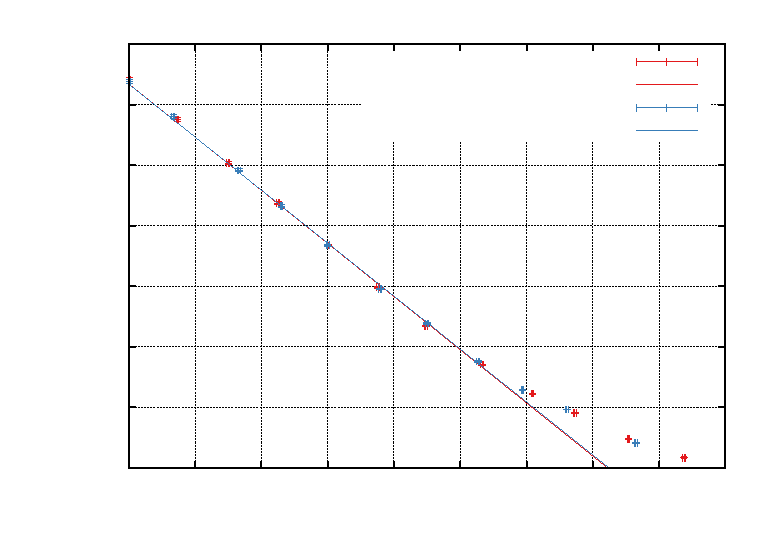
\includegraphics{./plots/photo/kennlinien_546nm}}%
    \gplfronttext
  \end{picture}%
\endgroup

	\caption{Linearisierte Kennlinie zur Grenzspannungsbestimmung $\lambda = \SI{546}{\nano\metre}$}
	\label{fig:kennlinien_546nm}
\end{figure}

\begin{table}
	\centering
	\begin{subtable}{0.5\textwidth}
		\centering
		\vspace{0pt}
		\resizebox{0.95\columnwidth}{!}{%
			\begin{tabular}{SSS}
	\toprule
	{$U$ / \si{\volt}} & {$I-I_0$ / \si{\nano\ampere}} & {$\Delta (I-I_0)$ / \si{\nano\ampere}} \\
	\midrule
0.001 & 10.261 & 0.208 \\
0.073 & 8.261  & 0.168 \\
0.150 & 6.331  & 0.129 \\
0.225 & 4.771  & 0.098 \\
0.301 & 3.371  & 0.070 \\
0.376 & 2.221  & 0.047 \\
0.448 & 1.371  & 0.030 \\
0.533 & 0.721  & 0.017 \\
0.609 & 0.371  & 0.010 \\
0.673 & 0.201  & 0.006 \\
0.754 & 0.051  & 0.003 \\
0.838 & 0.001  & 0.003 \\
	\bottomrule
\end{tabular}

		}
		\caption{Messung 1}
	\end{subtable}%
	\begin{subtable}{0.5\textwidth}
		\centering
		\vspace{0pt}
		\resizebox{0.95\columnwidth}{!}{%
			\begin{tabular}{SSS}
	\toprule
	{$U$ / \si{\volt}} & {$I-I_0$ / \si{\nano\ampere}} & {$\Delta (I-I_0)$ / \si{\nano\ampere}} \\
	\midrule
0.001 & 10.185 & 0.206 \\
0.067 & 8.405  & 0.170 \\
0.166 & 6.035  & 0.123 \\
0.230 & 4.675  & 0.096 \\
0.300 & 3.385  & 0.070 \\
0.379 & 2.185  & 0.046 \\
0.450 & 1.425  & 0.031 \\
0.527 & 0.775  & 0.018 \\
0.594 & 0.415  & 0.011 \\
0.661 & 0.235  & 0.007 \\
0.765 & 0.045  & 0.003 \\
 & & \\
	\bottomrule
\end{tabular}

		}
		\caption{Messung 2}
	\end{subtable}

	\caption{Kennlinien der Photozelle f\"ur Licht der Wellenl\"ange $\lambda = \SI{546}{\nano\metre}$}
\end{table}



% Messung 578nm
\begin{figure}
	\centering
	% GNUPLOT: LaTeX picture with Postscript
\begingroup
  \makeatletter
  \providecommand\color[2][]{%
    \GenericError{(gnuplot) \space\space\space\@spaces}{%
      Package color not loaded in conjunction with
      terminal option `colourtext'%
    }{See the gnuplot documentation for explanation.%
    }{Either use 'blacktext' in gnuplot or load the package
      color.sty in LaTeX.}%
    \renewcommand\color[2][]{}%
  }%
  \providecommand\includegraphics[2][]{%
    \GenericError{(gnuplot) \space\space\space\@spaces}{%
      Package graphicx or graphics not loaded%
    }{See the gnuplot documentation for explanation.%
    }{The gnuplot epslatex terminal needs graphicx.sty or graphics.sty.}%
    \renewcommand\includegraphics[2][]{}%
  }%
  \providecommand\rotatebox[2]{#2}%
  \@ifundefined{ifGPcolor}{%
    \newif\ifGPcolor
    \GPcolortrue
  }{}%
  \@ifundefined{ifGPblacktext}{%
    \newif\ifGPblacktext
    \GPblacktexttrue
  }{}%
  % define a \g@addto@macro without @ in the name:
  \let\gplgaddtomacro\g@addto@macro
  % define empty templates for all commands taking text:
  \gdef\gplbacktext{}%
  \gdef\gplfronttext{}%
  \makeatother
  \ifGPblacktext
    % no textcolor at all
    \def\colorrgb#1{}%
    \def\colorgray#1{}%
  \else
    % gray or color?
    \ifGPcolor
      \def\colorrgb#1{\color[rgb]{#1}}%
      \def\colorgray#1{\color[gray]{#1}}%
      \expandafter\def\csname LTw\endcsname{\color{white}}%
      \expandafter\def\csname LTb\endcsname{\color{black}}%
      \expandafter\def\csname LTa\endcsname{\color{black}}%
      \expandafter\def\csname LT0\endcsname{\color[rgb]{1,0,0}}%
      \expandafter\def\csname LT1\endcsname{\color[rgb]{0,1,0}}%
      \expandafter\def\csname LT2\endcsname{\color[rgb]{0,0,1}}%
      \expandafter\def\csname LT3\endcsname{\color[rgb]{1,0,1}}%
      \expandafter\def\csname LT4\endcsname{\color[rgb]{0,1,1}}%
      \expandafter\def\csname LT5\endcsname{\color[rgb]{1,1,0}}%
      \expandafter\def\csname LT6\endcsname{\color[rgb]{0,0,0}}%
      \expandafter\def\csname LT7\endcsname{\color[rgb]{1,0.3,0}}%
      \expandafter\def\csname LT8\endcsname{\color[rgb]{0.5,0.5,0.5}}%
    \else
      % gray
      \def\colorrgb#1{\color{black}}%
      \def\colorgray#1{\color[gray]{#1}}%
      \expandafter\def\csname LTw\endcsname{\color{white}}%
      \expandafter\def\csname LTb\endcsname{\color{black}}%
      \expandafter\def\csname LTa\endcsname{\color{black}}%
      \expandafter\def\csname LT0\endcsname{\color{black}}%
      \expandafter\def\csname LT1\endcsname{\color{black}}%
      \expandafter\def\csname LT2\endcsname{\color{black}}%
      \expandafter\def\csname LT3\endcsname{\color{black}}%
      \expandafter\def\csname LT4\endcsname{\color{black}}%
      \expandafter\def\csname LT5\endcsname{\color{black}}%
      \expandafter\def\csname LT6\endcsname{\color{black}}%
      \expandafter\def\csname LT7\endcsname{\color{black}}%
      \expandafter\def\csname LT8\endcsname{\color{black}}%
    \fi
  \fi
  \setlength{\unitlength}{0.0500bp}%
  \begin{picture}(7200.00,5040.00)%
    \gplgaddtomacro\gplbacktext{%
      \csname LTb\endcsname%
      \put(946,704){\makebox(0,0)[r]{\strut{} 0}}%
      \csname LTb\endcsname%
      \put(946,1518){\makebox(0,0)[r]{\strut{} 0.5}}%
      \csname LTb\endcsname%
      \put(946,2332){\makebox(0,0)[r]{\strut{} 1}}%
      \csname LTb\endcsname%
      \put(946,3147){\makebox(0,0)[r]{\strut{} 1.5}}%
      \csname LTb\endcsname%
      \put(946,3961){\makebox(0,0)[r]{\strut{} 2}}%
      \csname LTb\endcsname%
      \put(946,4775){\makebox(0,0)[r]{\strut{} 2.5}}%
      \csname LTb\endcsname%
      \put(1078,484){\makebox(0,0){\strut{} 0}}%
      \csname LTb\endcsname%
      \put(1794,484){\makebox(0,0){\strut{} 0.1}}%
      \csname LTb\endcsname%
      \put(2509,484){\makebox(0,0){\strut{} 0.2}}%
      \csname LTb\endcsname%
      \put(3225,484){\makebox(0,0){\strut{} 0.3}}%
      \csname LTb\endcsname%
      \put(3941,484){\makebox(0,0){\strut{} 0.4}}%
      \csname LTb\endcsname%
      \put(4656,484){\makebox(0,0){\strut{} 0.5}}%
      \csname LTb\endcsname%
      \put(5372,484){\makebox(0,0){\strut{} 0.6}}%
      \csname LTb\endcsname%
      \put(6087,484){\makebox(0,0){\strut{} 0.7}}%
      \csname LTb\endcsname%
      \put(6803,484){\makebox(0,0){\strut{} 0.8}}%
      \put(176,2739){\rotatebox{-270}{\makebox(0,0){\strut{}$\sqrt{I-I_0} \, / \, \si{\nano\ampere^{1/2}}$}}}%
      \put(3940,154){\makebox(0,0){\strut{}$U \, / \, \si{\volt}$}}%
      \put(3940,4665){\makebox(0,0){\strut{}}}%
    }%
    \gplgaddtomacro\gplfronttext{%
      \csname LTb\endcsname%
      \put(5816,4602){\makebox(0,0)[r]{\strut{}Messung 1}}%
      \csname LTb\endcsname%
      \put(5816,4382){\makebox(0,0)[r]{\strut{}Regressionsgerade 1}}%
      \csname LTb\endcsname%
      \put(5816,4162){\makebox(0,0)[r]{\strut{}Messung 2}}%
      \csname LTb\endcsname%
      \put(5816,3942){\makebox(0,0)[r]{\strut{}Regressionsgerade 2}}%
    }%
    \gplbacktext
    \put(0,0){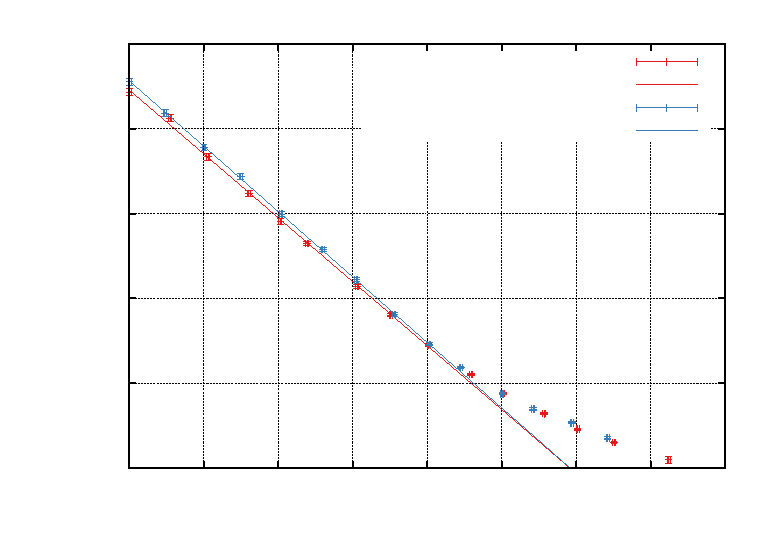
\includegraphics{./plots/photo/kennlinien_578nm}}%
    \gplfronttext
  \end{picture}%
\endgroup

	\caption{Linearisierte Kennlinie zur Grenzspannungsbestimmung $\lambda = \SI{578}{\nano\metre}$}
	\label{fig:kennlinien_578nm}
\end{figure}

\begin{table}
	\centering
	\begin{subtable}{0.5\textwidth}
		\centering
		\vspace{0pt}
		\resizebox{0.95\columnwidth}{!}{%
			\begin{tabular}{SSS}
	\toprule
	{$U$ / \si{\volt}} & {$I-I_0$ / \si{\nano\ampere}} & {$\Delta (I-I_0)$ / \si{\nano\ampere}} \\
	\midrule
0.001 & 4.913 & 0.101 \\
0.055 & 4.253 & 0.087 \\
0.106 & 3.363 & 0.070 \\
0.161 & 2.623 & 0.055 \\
0.203 & 2.113 & 0.045 \\
0.239 & 1.753 & 0.037 \\
0.306 & 1.143 & 0.025 \\
0.351 & 0.813 & 0.019 \\
0.402 & 0.523 & 0.013 \\
0.459 & 0.303 & 0.008 \\
0.502 & 0.193 & 0.006 \\
0.557 & 0.103 & 0.004 \\
0.602 & 0.053 & 0.003 \\
0.651 & 0.023 & 0.003 \\
0.724 & 0.003 & 0.003 \\
	\bottomrule
\end{tabular}

		}
		\caption{Messung 1}
	\end{subtable}%
	\begin{subtable}{0.5\textwidth}
		\centering
		\vspace{0pt}
		\resizebox{0.95\columnwidth}{!}{%
			\begin{tabular}{SSS}
	\toprule
	{$U$ / \si{\volt}} & {$I-I_0$ / \si{\nano\ampere}} & {$\Delta (I-I_0)$ / \si{\nano\ampere}} \\
	\midrule
0.001 & 5.181 & 0.106 \\
0.048 & 4.371 & 0.090 \\
0.101 & 3.571 & 0.074 \\
0.150 & 2.951 & 0.061 \\
0.204 & 2.241 & 0.047 \\
0.260 & 1.661 & 0.036 \\
0.305 & 1.231 & 0.027 \\
0.356 & 0.821 & 0.019 \\
0.403 & 0.531 & 0.013 \\
0.445 & 0.351 & 0.009 \\
0.501 & 0.191 & 0.006 \\
0.542 & 0.121 & 0.005 \\
0.594 & 0.071 & 0.004 \\
0.642 & 0.031 & 0.003 \\
 & & \\
	\bottomrule
\end{tabular}

		}
		\caption{Messung 2}
	\end{subtable}

	\caption{Kennlinien der Photozelle f\"ur Licht der Wellenl\"ange $\lambda = \SI{578}{\nano\metre}$}
\end{table}




\end{appendix}

\end{document}
